\documentclass{article}
\usepackage{graphicx}
\usepackage{titlesec}
\usepackage{hyperref}
\usepackage{caption}
\usepackage{listings}
\usepackage{xcolor}
\usepackage[a4paper, margin=1in]{geometry}
\usepackage{float}
\usepackage{tocloft}

% Fix TOC page number alignment
\cftsetindents{subsection}{1.5em}{2.3em}
\setlength{\cftsecnumwidth}{4em}
\setlength{\cftsubsecnumwidth}{5em}

\begin{document}

\begin{titlepage}
    \centering
    
    % EPITA Logo
    
\includegraphics[width=0.4\textwidth]{figures/Epita.jpg} \\
    \vspace{1.5cm}
    
    % Program
    {\large Master in Computer Science} \\
    {\large Software Engineering} \\
    

    
    % Main Title
        \vspace{0.5cm}
    {\Huge \textbf{Cloud Computing}} \\
    \vspace{1.3cm}
    {\huge Report 1}
        \vspace{0.1cm}

    
    % Team Members
    {\Large \textbf{Team Members}} \\
    \vspace{0.5cm}
    {\large Jordy Meye} \\
    {\large Huizhe Su} \\
    {\large Arihant Jain} \\
    {\large Nizar} \\
    
    \vspace{1.5cm}
    {\large February 2026}

\end{titlepage}


\newpage
% --- Styling --- %
\titleformat{\section}
  {\Large\bfseries}
  {Exercise \arabic{section}.}
  {1em}
  {}

\titleformat{\subsection}
  {\normalsize\bfseries}
  {Question \arabic{subsection}.}
  {1em}
  {}

% Code listing style
\lstset{
    basicstyle=\ttfamily\small,
    backgroundcolor=\color{gray!10},
    frame=single,
    breaklines=true,
    postbreak=\mbox{\textcolor{red}{$\hookrightarrow$}\space},
    showstringspaces=false,
    tabsize=4,
    xleftmargin=2em,
    framexleftmargin=1.5em,
}

\raggedbottom
\setlength{\intextsep}{6pt plus 2pt minus 2pt}
\setlength{\floatsep}{6pt plus 2pt minus 2pt}
\setlength{\textfloatsep}{6pt plus 2pt minus 2pt}



\tableofcontents
\newpage

%% ============ SECTION 1: Server Installation ============ %%
\section{Server Installation}

\subsection{Install Ubuntu 18.04 LTS in Amazon EC2}
After registering on AWS and setting up an EC2 instance, we have the following information page.

\begin{figure}[H]
\centering
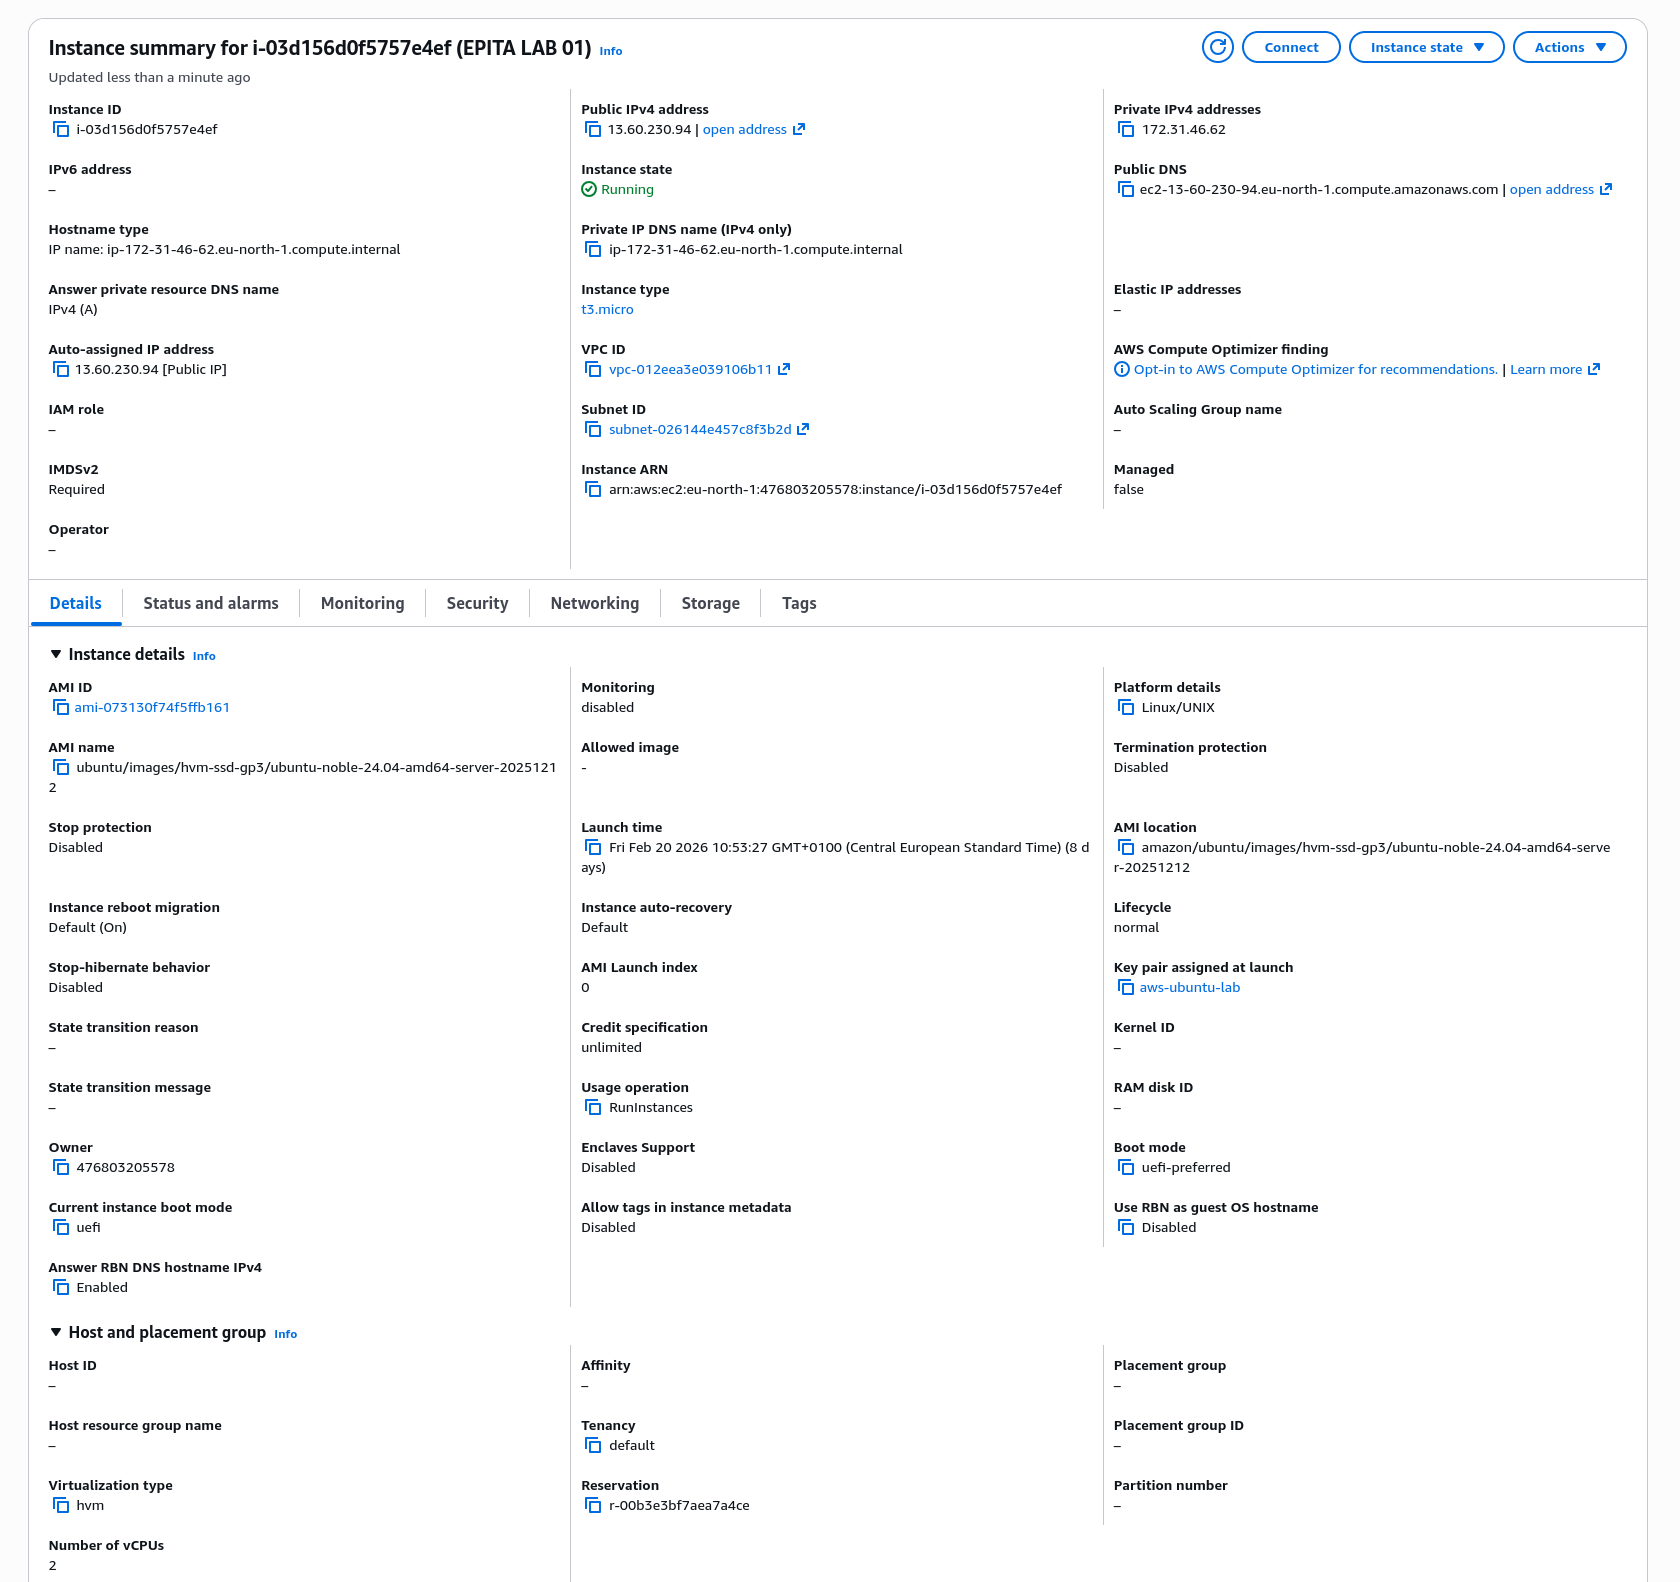
\includegraphics[width=0.65\textwidth]{figures/ec2.png}
\caption{AWS EC instance information page (Huizhe Su)}
\end{figure}
It's recommanded to use ssh to login to the remote server. First, we download our ssh key from our account, then we need to change the permission of the private key to be read-only by user only.
\begin{lstlisting}[language=bash]
chmod 400 ./aws-ubuntu-lab.pem
\end{lstlisting}
For easy access our remote server, we can edit \texttt{~/.ssh/config} and add the following configuration.
\begin{lstlisting}
Host aws_epita
    HostName ec2-13-60-230-94.eu-north-1.compute.amazonaws.com
    User ubuntu
    IdentityFile ~/.ssh/aws-ubuntu-lab.pem
\end{lstlisting}
\subsection{Update the system}
We update the server using the following command:
\begin{lstlisting}[language=bash]
sudo apt-get install update
sudp apt-get install upgrade
\end{lstlisting}

\subsection{Find the main characteristics of your instance from the commands below.}

Instead of output the information by command line, we can use a new tool called \texttt{neofetch}. Install neofetch and run neofetch
\begin{lstlisting}[language=bash]
sudo apt-get install neofetch
neofetch
\end{lstlisting}
Then we will get the information
\begin{figure}[H]
    \centering
    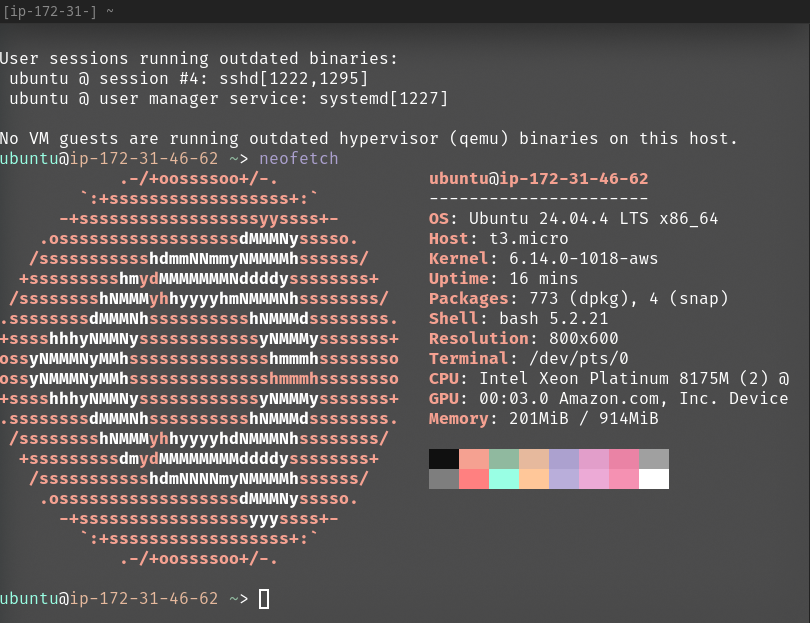
\includegraphics[width=0.65\textwidth]{figures/neofetch.png}
    \caption{Neofetch and system infromation (Huizhe Su)}
\end{figure}
For other information, we selected to show \texttt{ssh} logs, network interfaces, detailed CPU infomation, installed packages, groups, passwd, devices, processes, fire wall status, hardware space.
\begin{lstlisting}[language=bash]
journalctl -u ssh # log for ssh
ifconfig #network interfaces
cat /proc/cpuinfo # cpu info
dpkg -l | wc -l # calculate installed packages
# we use getent instead of cat for accessing sytem database
getent group  # groups
getent passwd # passwd
lsusb # list usb devices
lspci # list pheripheral devices
top # snapshot of current processes
ps x # list all processes
sudo ufw status verbose # show firewall status
df -l --si # hardware spaces
\end{lstlisting}
\begin{figure}[H]
    \centering
    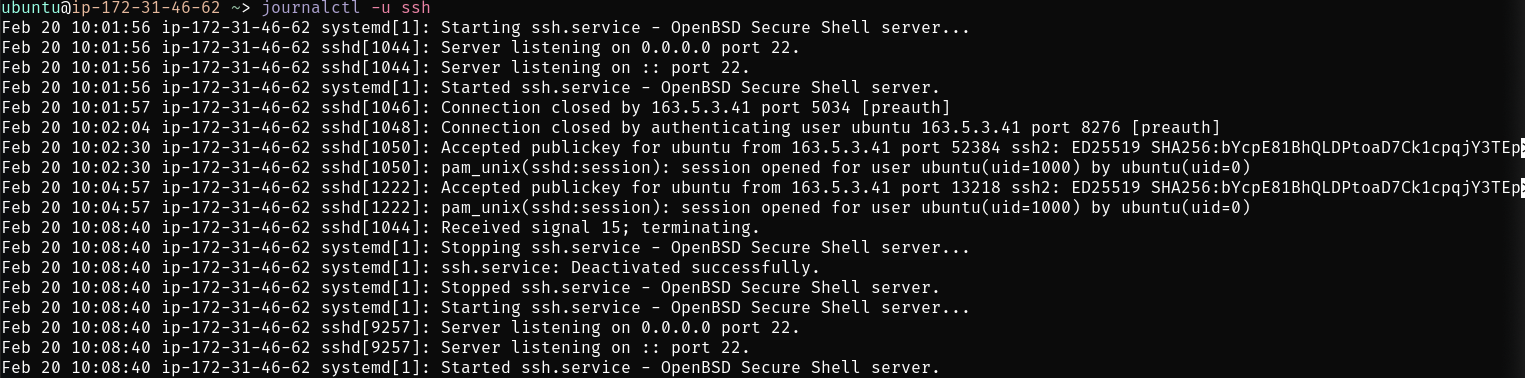
\includegraphics[width=0.65\textwidth]{figures/journalctl_ssh.png}
    \caption{User level logs of ssh service(Huizhe Su)}
\end{figure}
\begin{figure}[H]
    \centering
    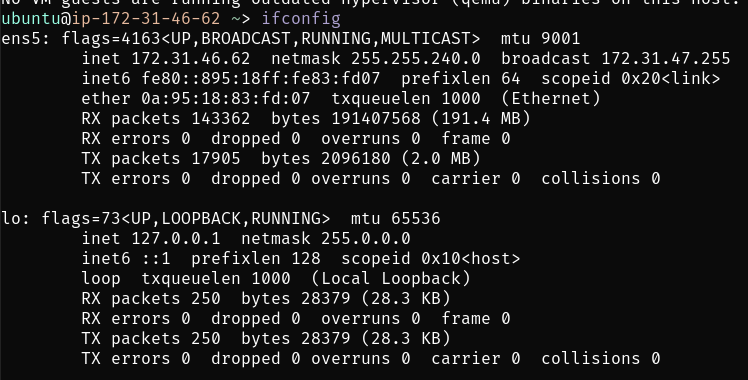
\includegraphics[width=0.65\textwidth]{figures/ifconfig.png}
    \caption{Network interfaces (Huizhe Su)}
\end{figure}
\begin{figure}[H]
    \centering
    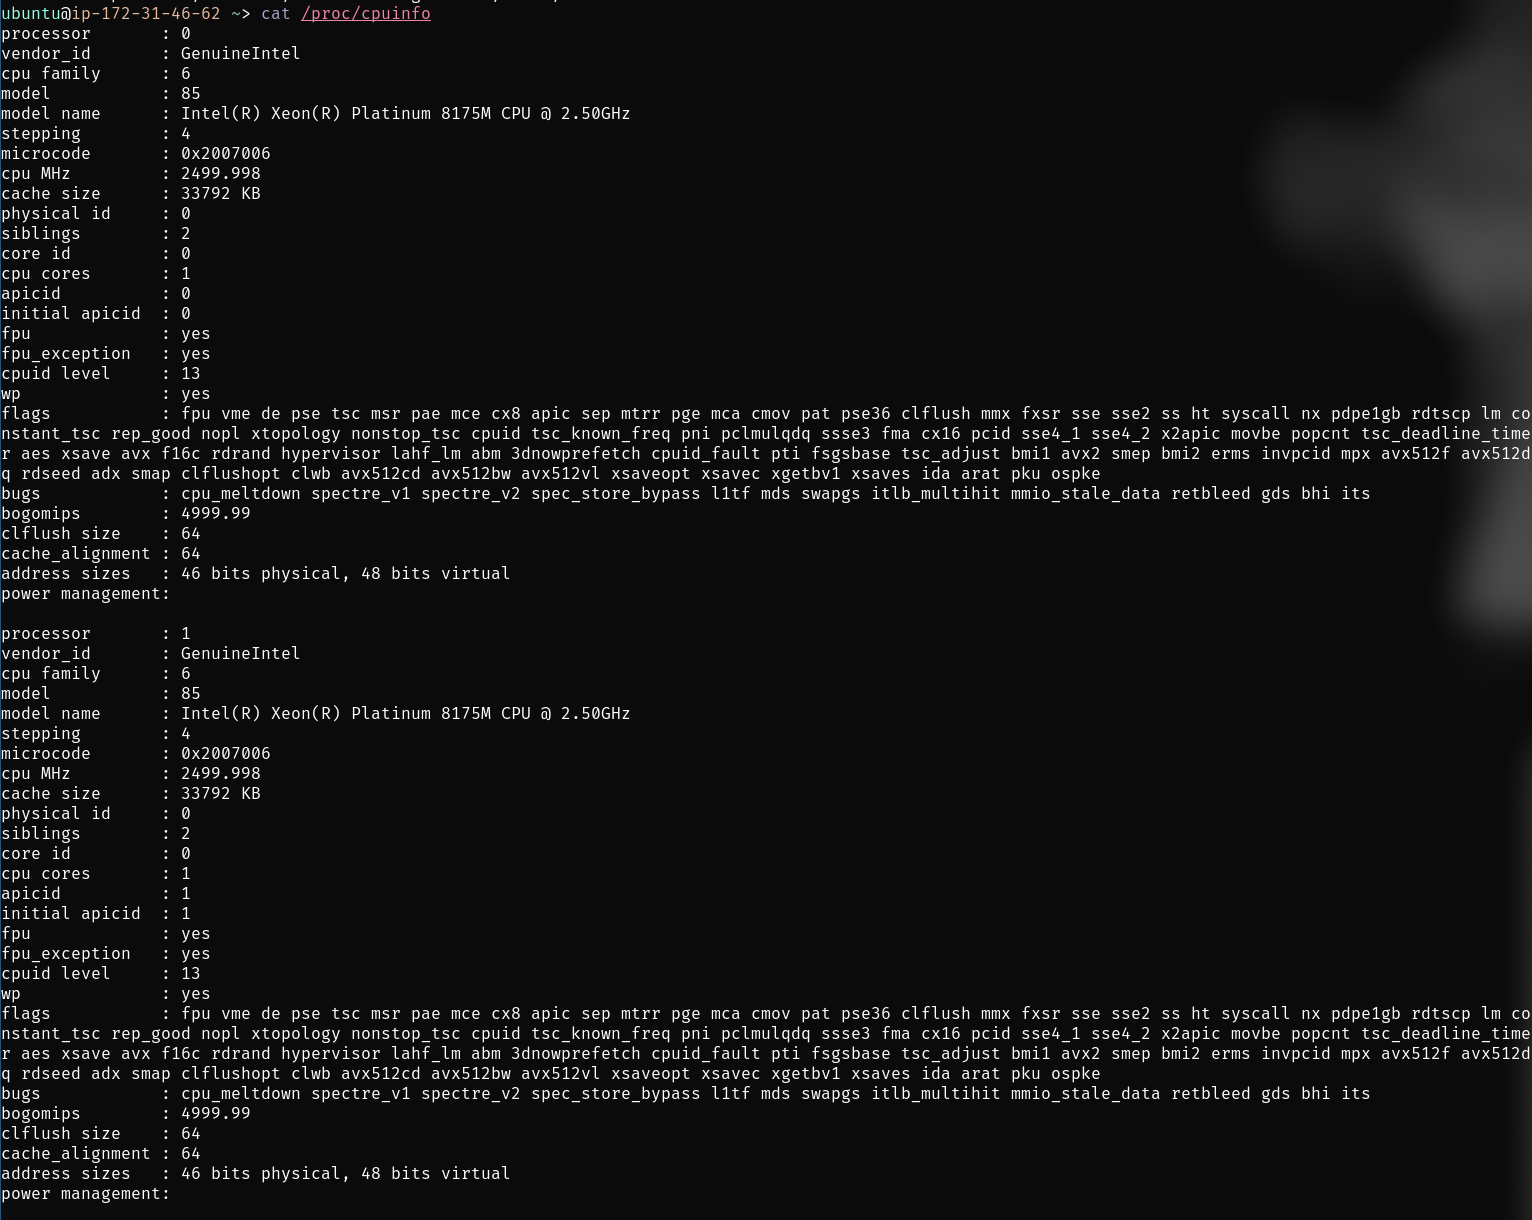
\includegraphics[width=0.65\textwidth]{figures/cpuinfo.png}
    \caption{Detailed CPU information (Huizhe Su)}
\end{figure}
\begin{figure}[H]
    \centering
    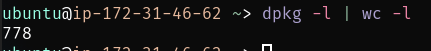
\includegraphics[width=0.65\textwidth]{figures/dpkg.png}
    \caption{There are 778 installed packages (Huizhe Su)}
\end{figure}
\begin{figure}[H]
    \centering
    \begin{minipage}{0.45\textwidth}
        \centering
        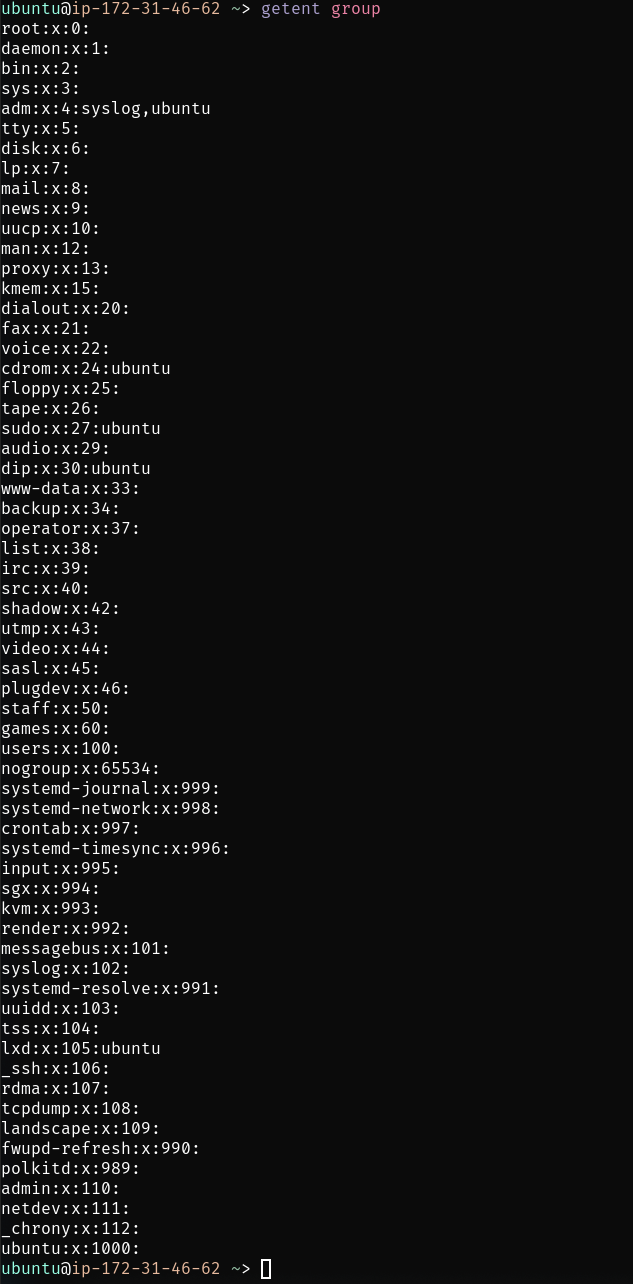
\includegraphics[width=\textwidth]{figures/group.png}
        \captionof{figure}{Group information}
    \end{minipage}
    \begin{minipage}{0.45\textwidth}
        \centering
        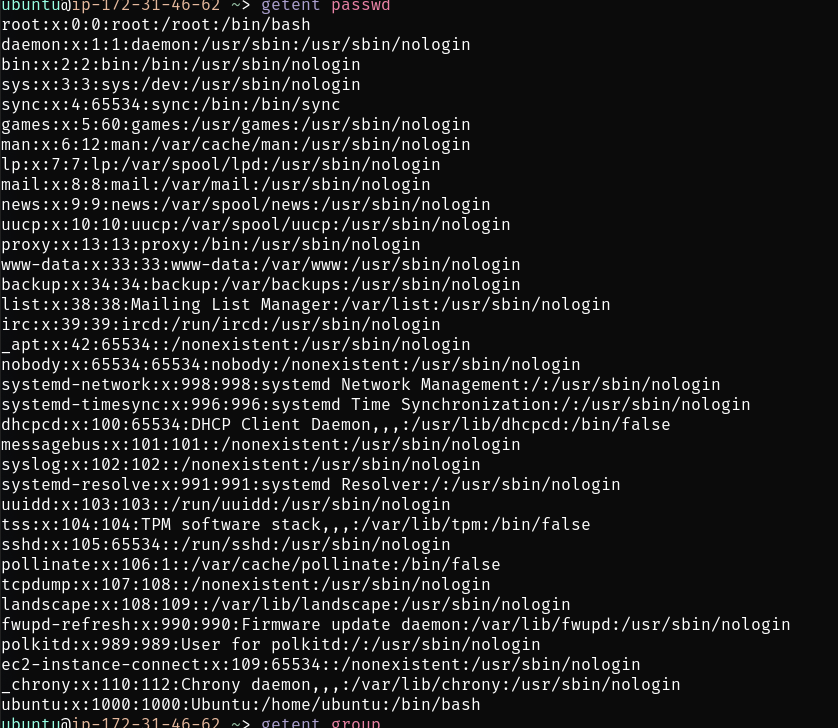
\includegraphics[width=\textwidth]{figures/passwd.png}
        \captionof{figure}{User informaiton}
    \end{minipage}
\end{figure}
\begin{figure}[H]
    \centering
    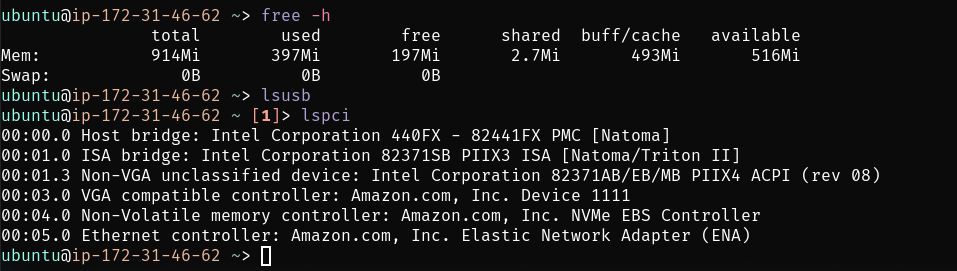
\includegraphics[width=0.65\textwidth]{figures/lspci.png}
    \caption{USB information and pheripheral information (Huizhe Su)}
\end{figure}
\begin{figure}[H]
    \centering
    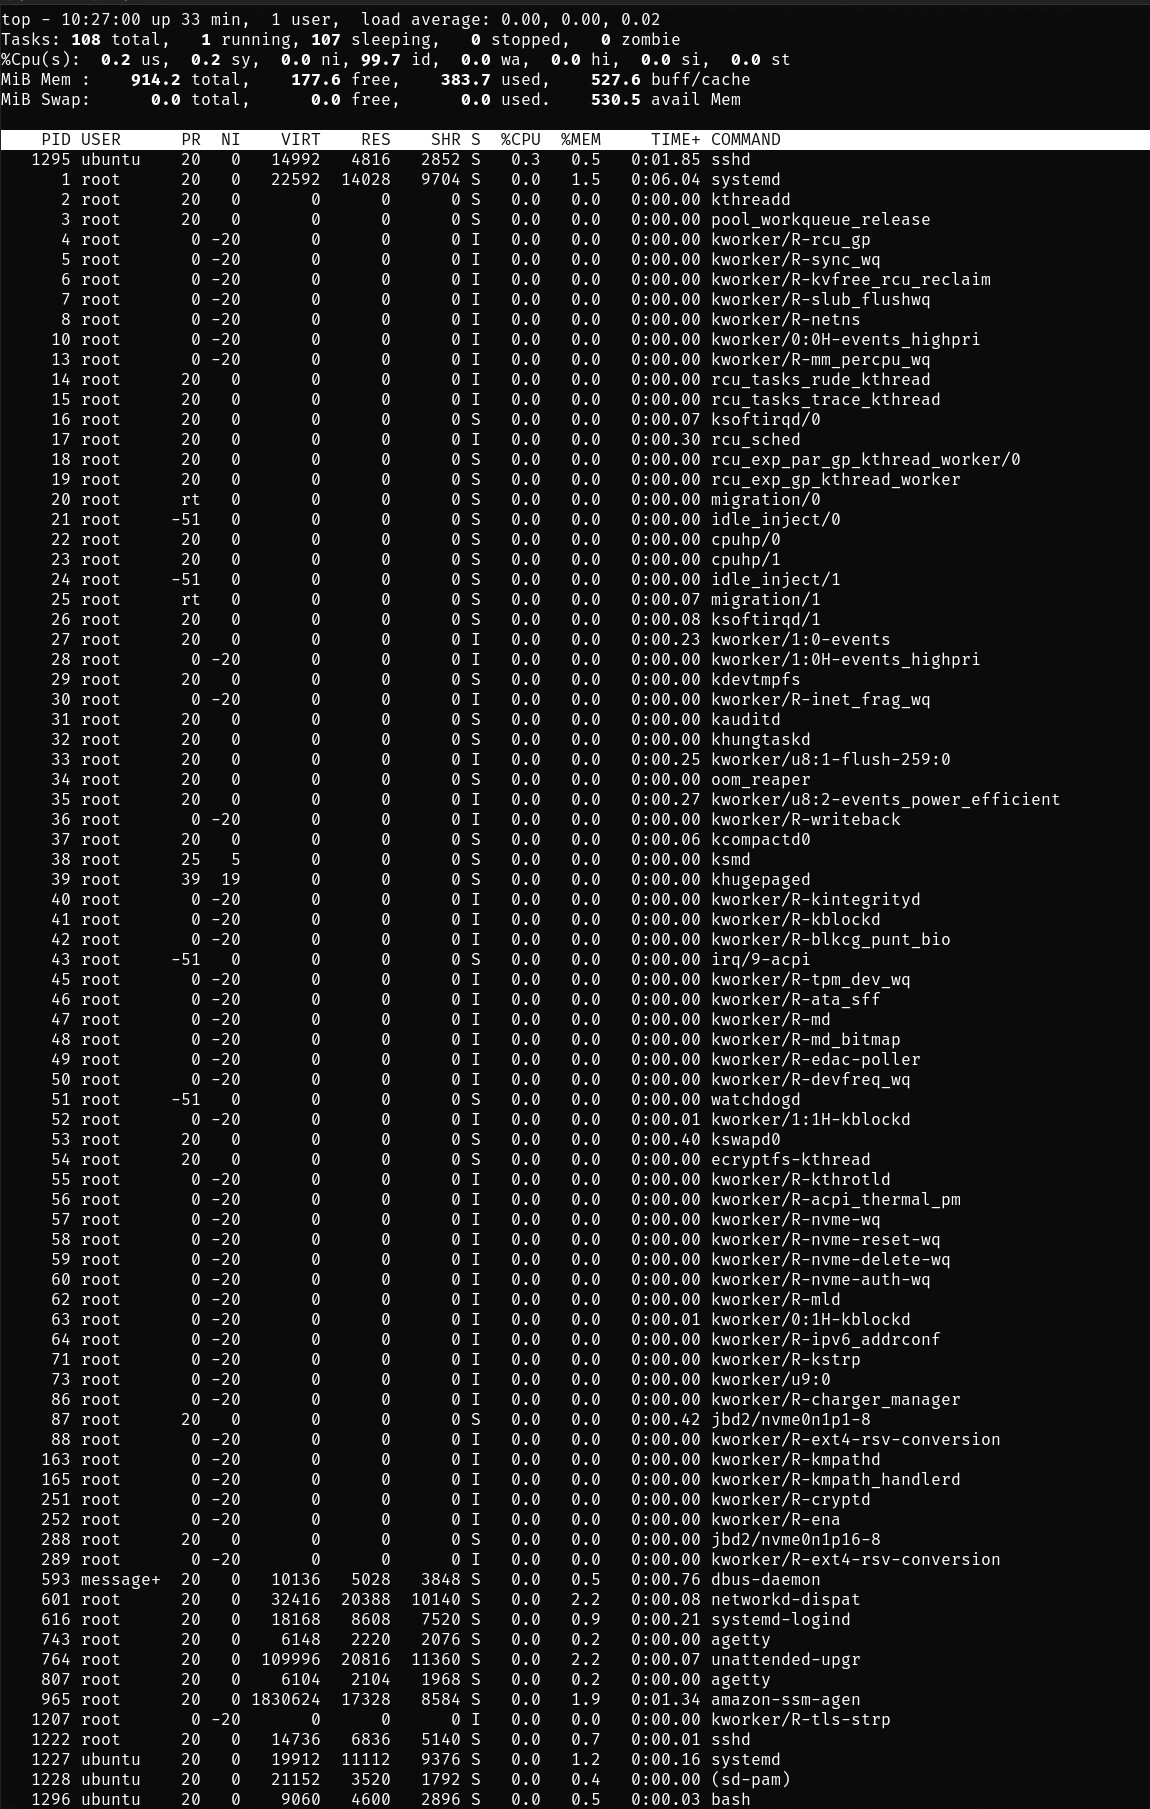
\includegraphics[width=0.65\textwidth]{figures/top.png}
    \caption{current processes (using \texttt{top}) (Huizhe Su)}
\end{figure}
\begin{figure}[H]
    \centering
    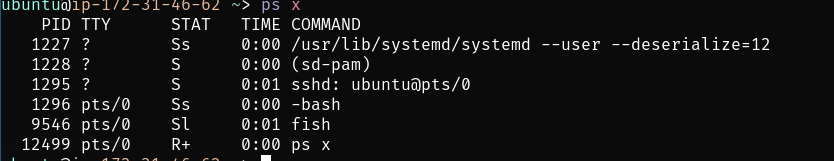
\includegraphics[width=0.65\textwidth]{figures/ps.png}
    \caption{current processes (using \texttt{ps}) (Huizhe Su)}
\end{figure}
\begin{figure}[H]
    \centering
    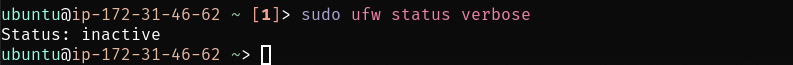
\includegraphics[width=0.65\textwidth]{figures/ufw.png}
    \caption{Firewall status (closed) (Huizhe Su)}
\end{figure}
\begin{figure}[H]
    \centering
    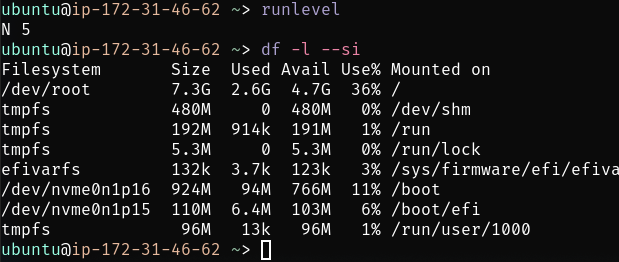
\includegraphics[width=0.65\textwidth]{figures/df_runlevel.png}
    \caption{Free space on disk (Huizhe Su)}
\end{figure}
%% ============ SECTION 2: Installing Apache Web Server ============ %%
\section{Installing Apache Web Server}
\setcounter{subsection}{3}

\subsection{Install the Apache 2 HTTP Server}
To serve web content from our EC2 instance, we install the Apache2 web server and enable the service so that it starts automatically on boot.

\begin{lstlisting}[language=bash]
sudo apt install apache2
sudo systemctl start apache2
sudo systemctl enable apache2
\end{lstlisting}

\begin{figure}[H]
    \centering
    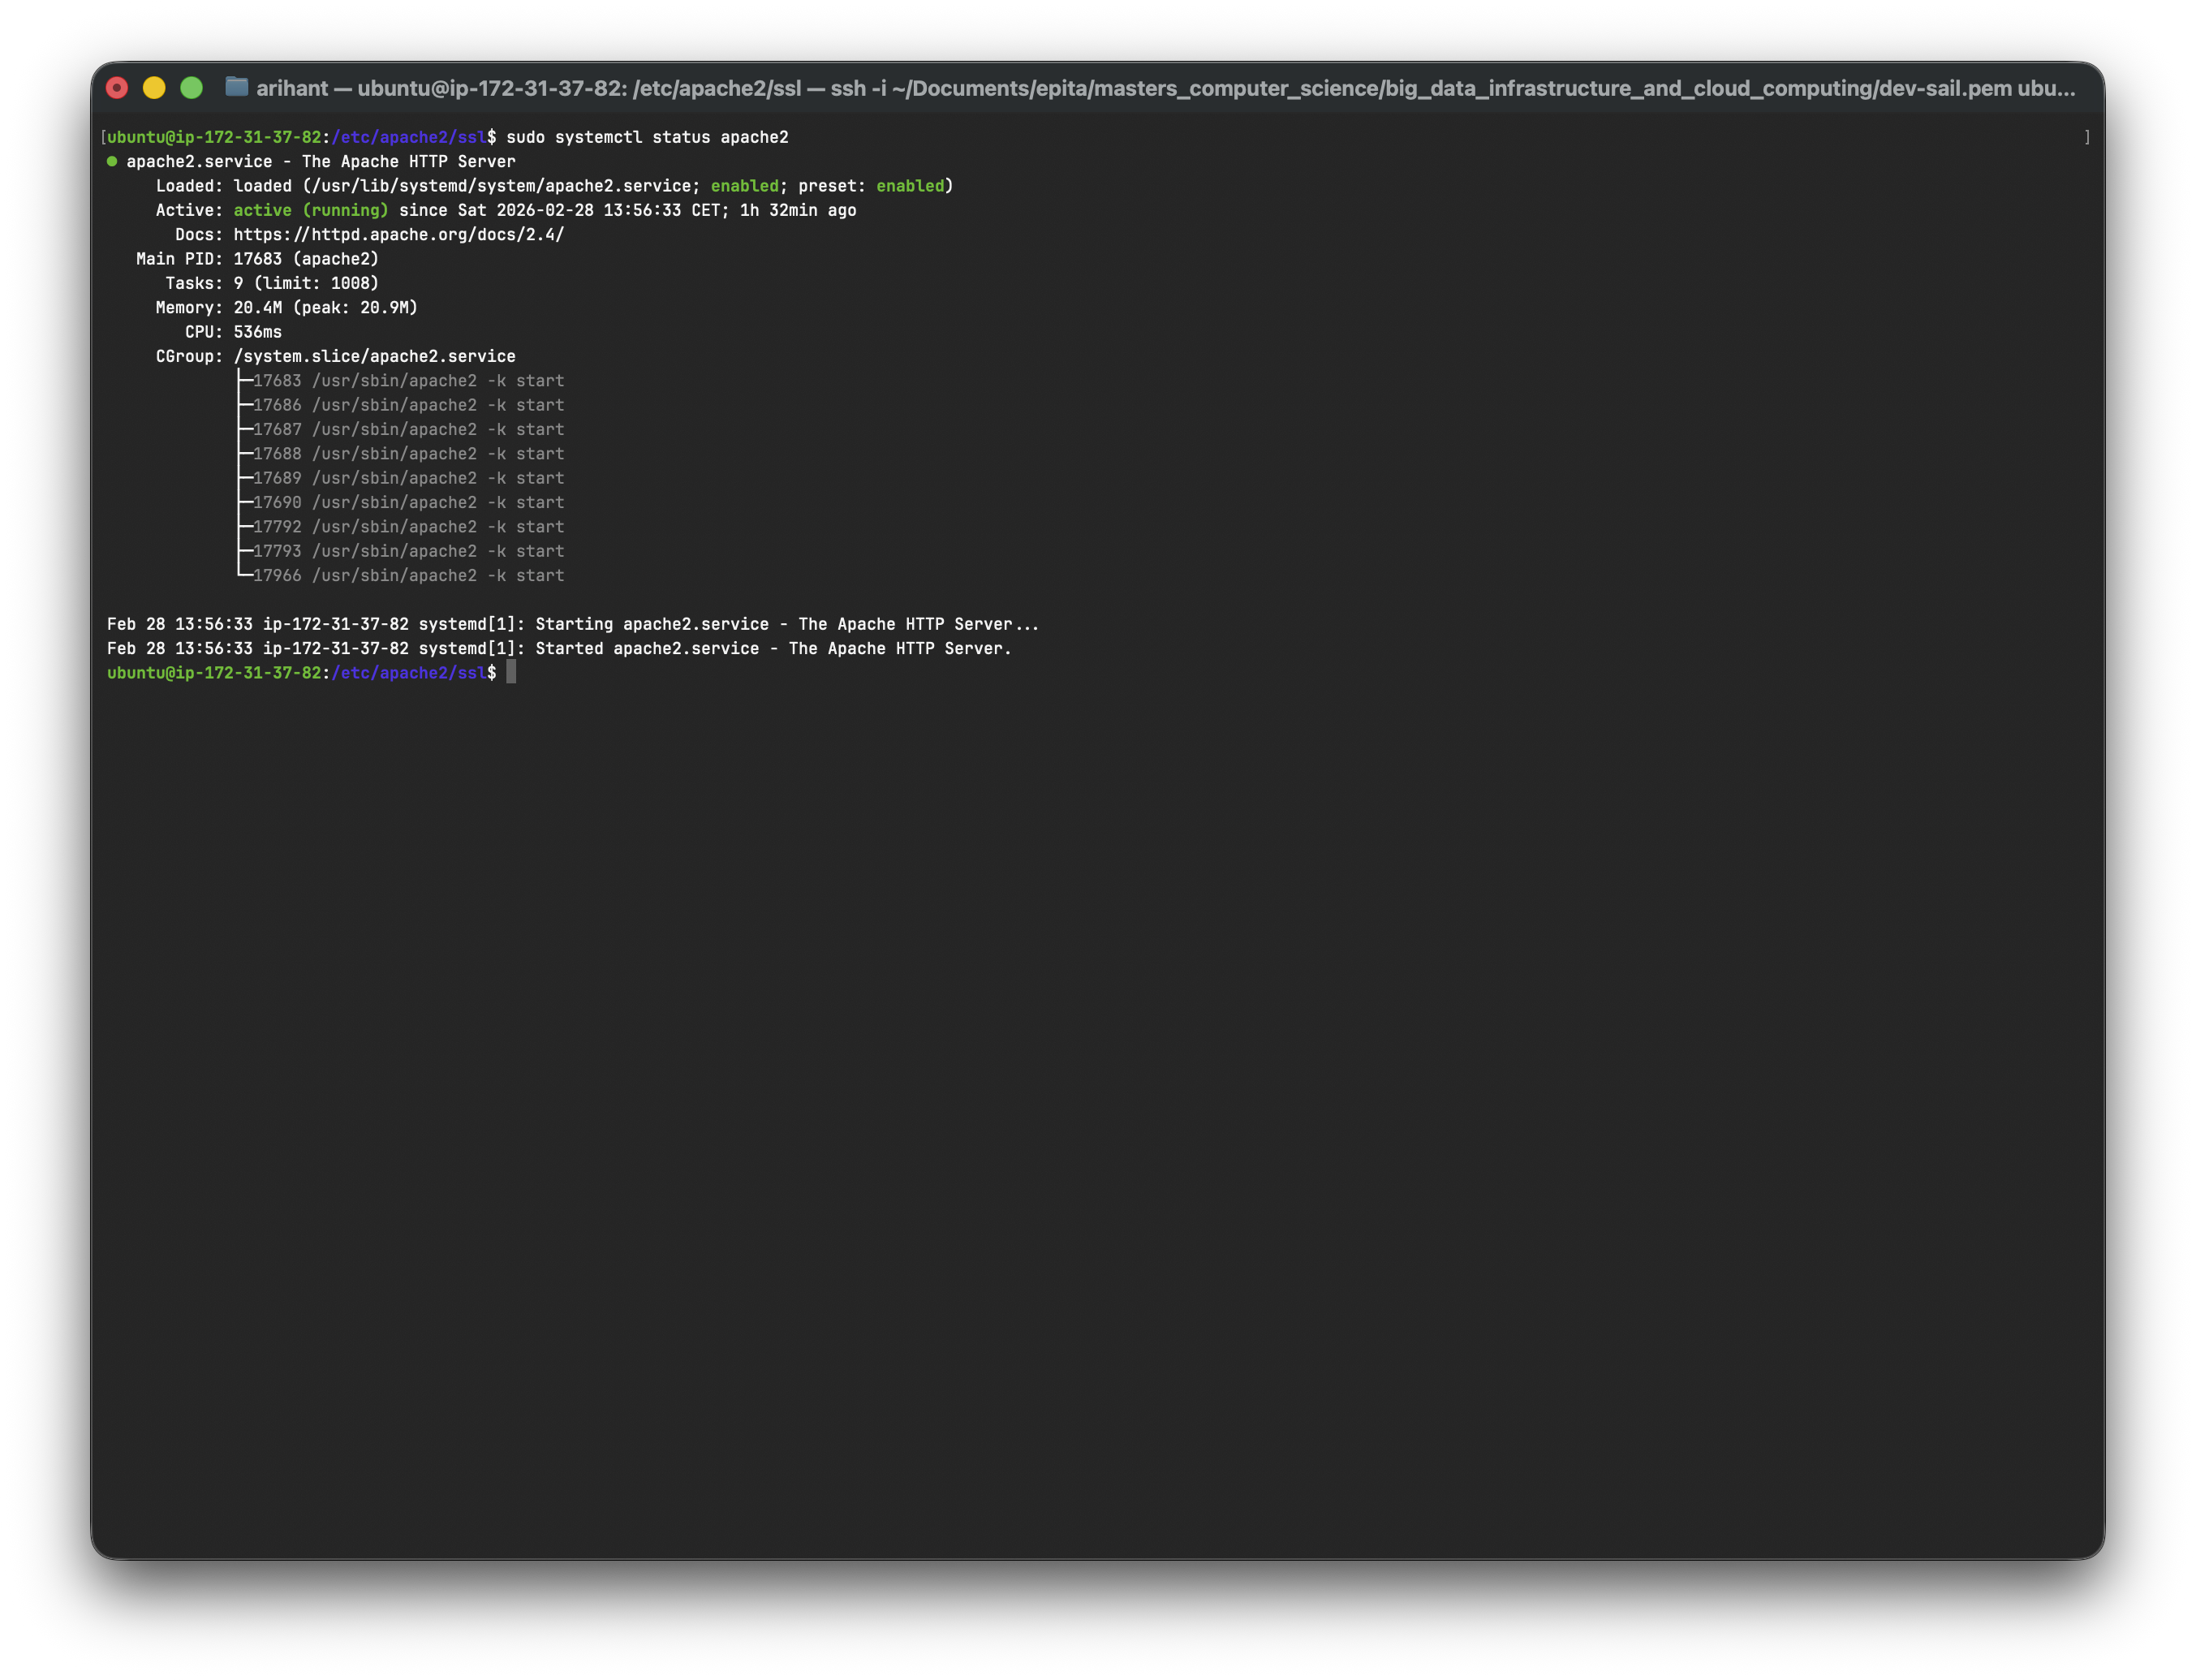
\includegraphics[width=0.65\textwidth]{figures/apache2_status.png}
    \caption{Apache2 service running successfully (Arihant Jain)}
\end{figure}

\subsection{Check the Status of Apache 2 and Give Its Version}
We can verify that Apache is running correctly and check its version:

\begin{lstlisting}[language=bash]
sudo systemctl status apache2
apache2 -v
\end{lstlisting}

The \texttt{systemctl status} command confirms that the service is \texttt{active (running)}. The \texttt{apache2 -v} command outputs the installed version:

\begin{lstlisting}
Server version: Apache/2.4.58 (Ubuntu)
Server built:   2025-12-09T15:50:28
\end{lstlisting}

\begin{figure}[H]
    \centering
    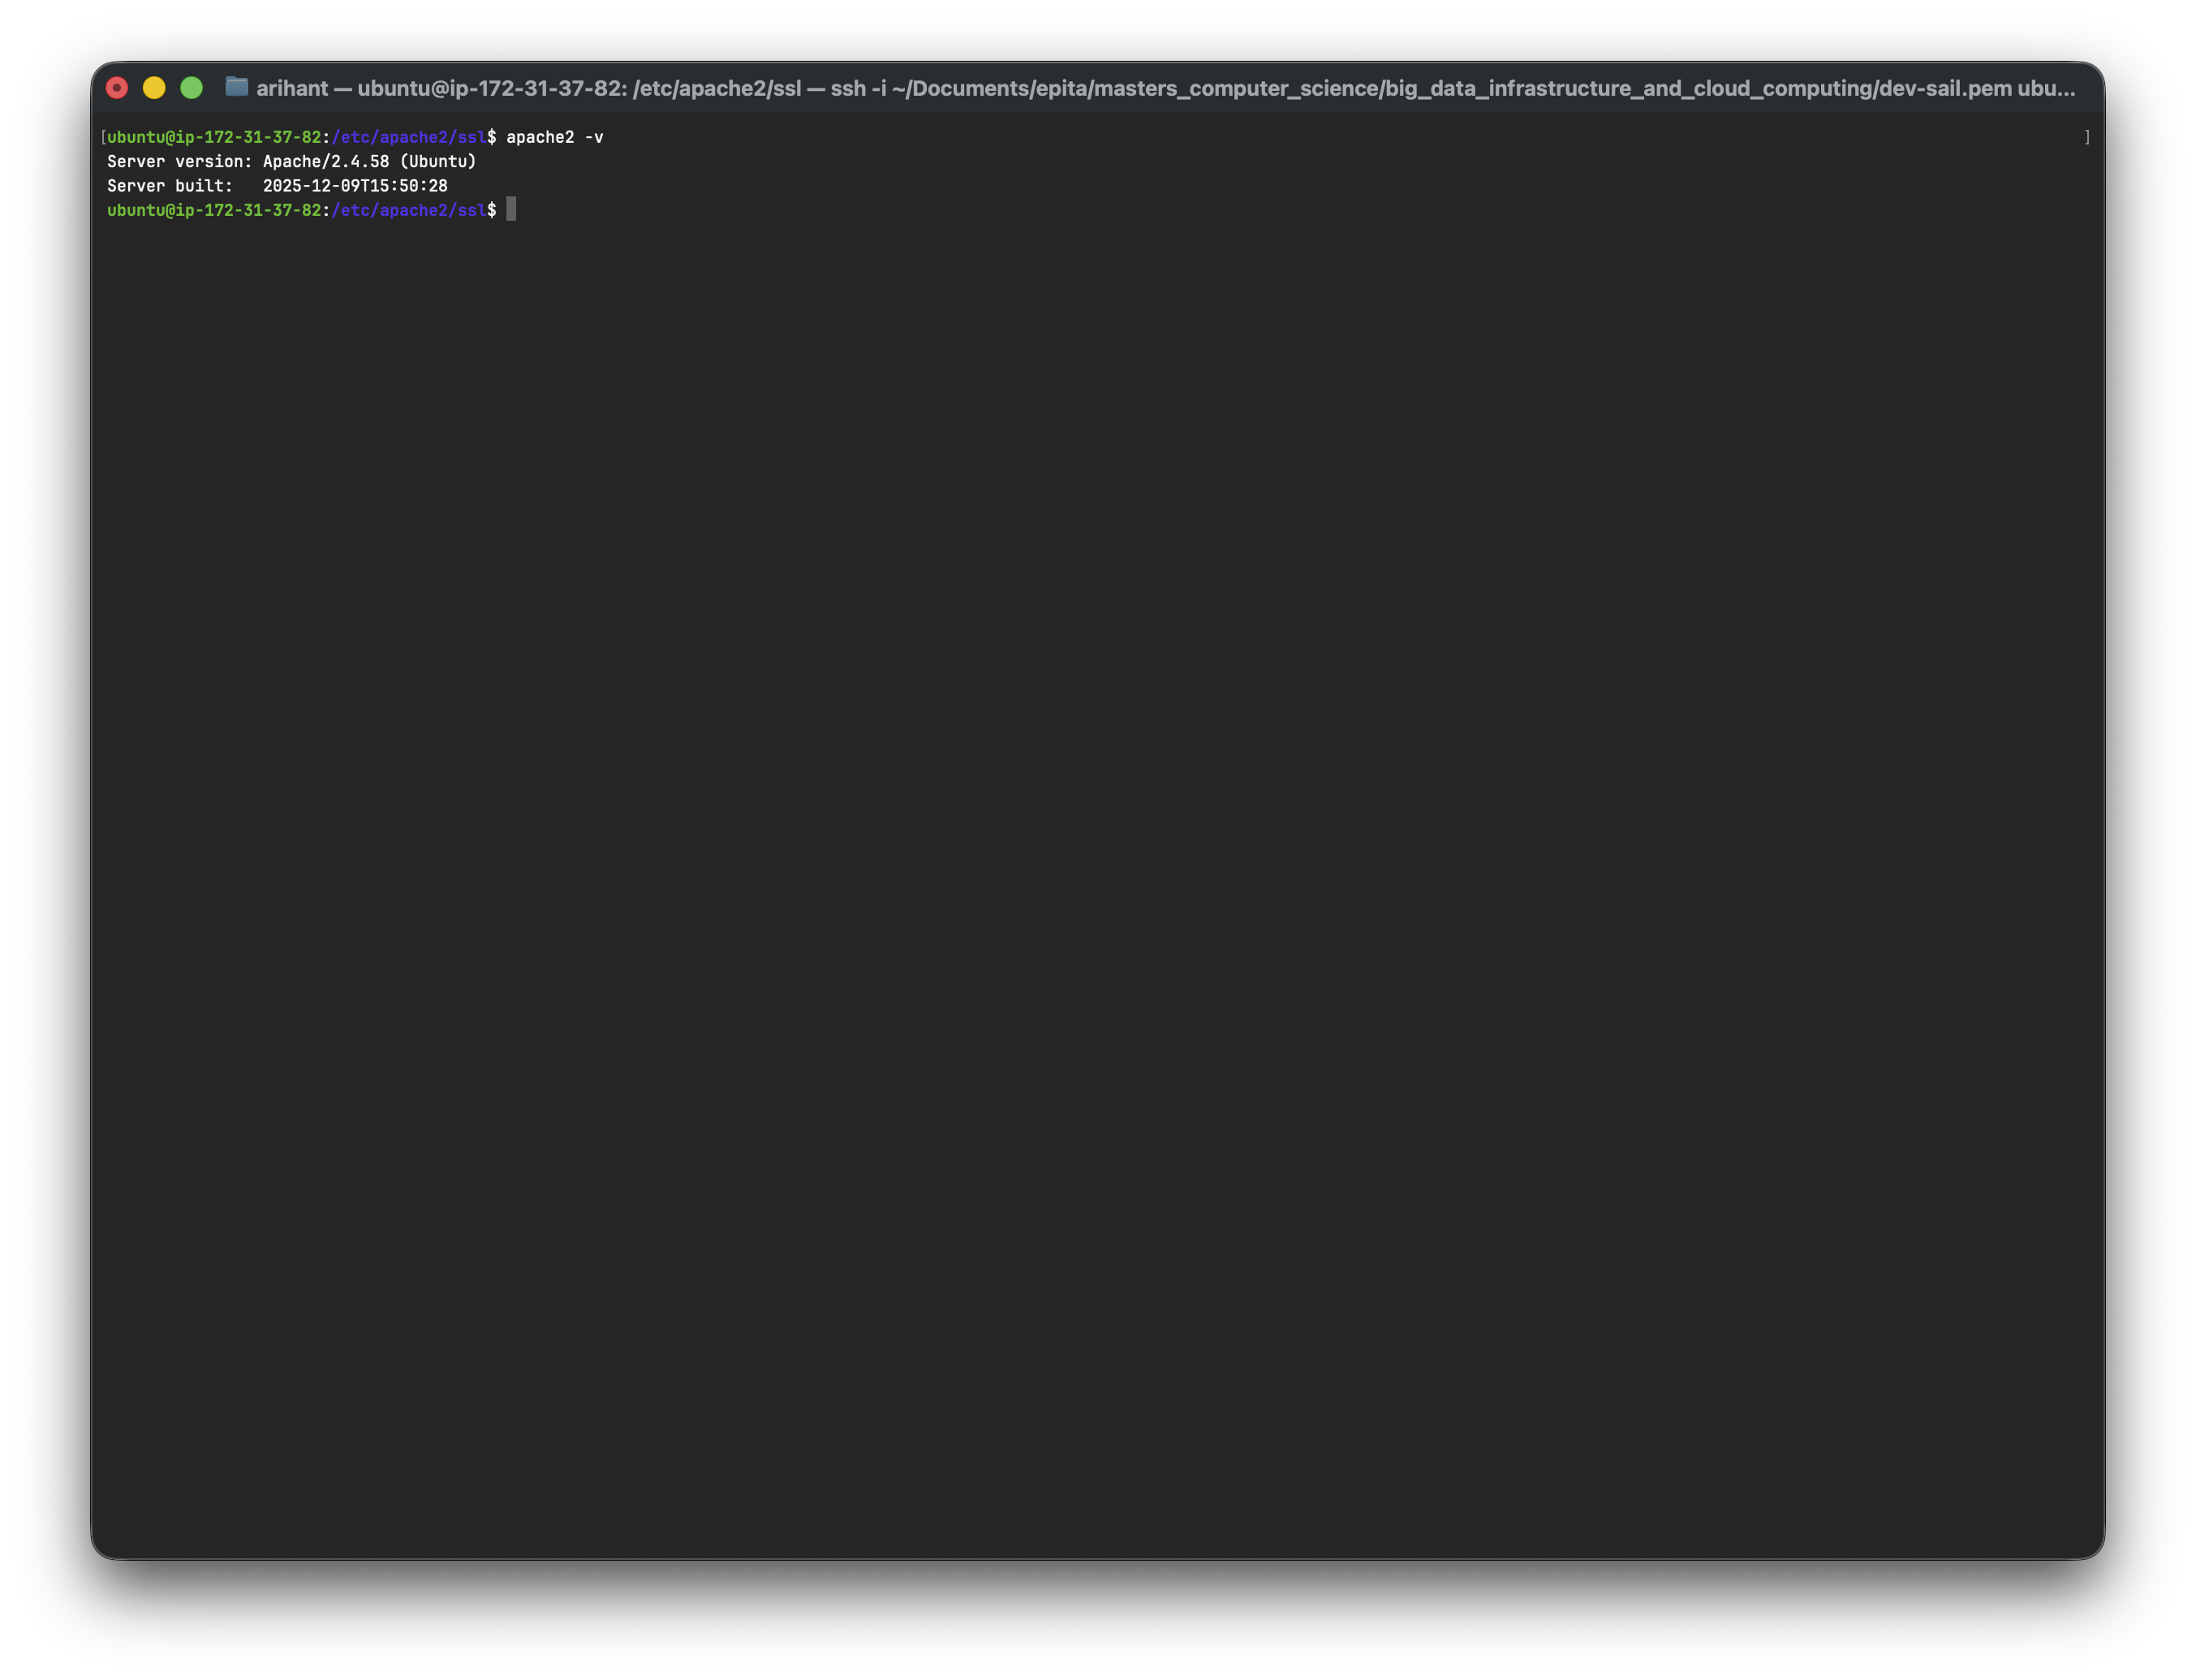
\includegraphics[width=0.65\textwidth]{figures/apache2_version.png}
    \caption{Apache2 version output (Arihant Jain)}
\end{figure}

\subsection{Create a Home Page and Test with a Web Browser}
With Apache running, the default page is accessible at:

\begin{center}
\texttt{http://ec2-35-180-10-25.eu-west-3.compute.amazonaws.com}
\end{center}

This serves the default Apache2 Ubuntu page located at \texttt{/var/www/html/index.html}. We then edited this file to serve our own content:

\begin{lstlisting}[language=bash]
sudo nano /var/www/html/index.html
\end{lstlisting}

We replaced the default content with a simple custom page:

\begin{lstlisting}[language=HTML]
<html>
    <head>
        <title>My Server</title>
    </head>
    <body>
        Bienvenue sur mon serveur
    </body>
</html>
\end{lstlisting}

After saving the file, refreshing the browser shows our custom page.

\begin{figure}[H]
    \centering
    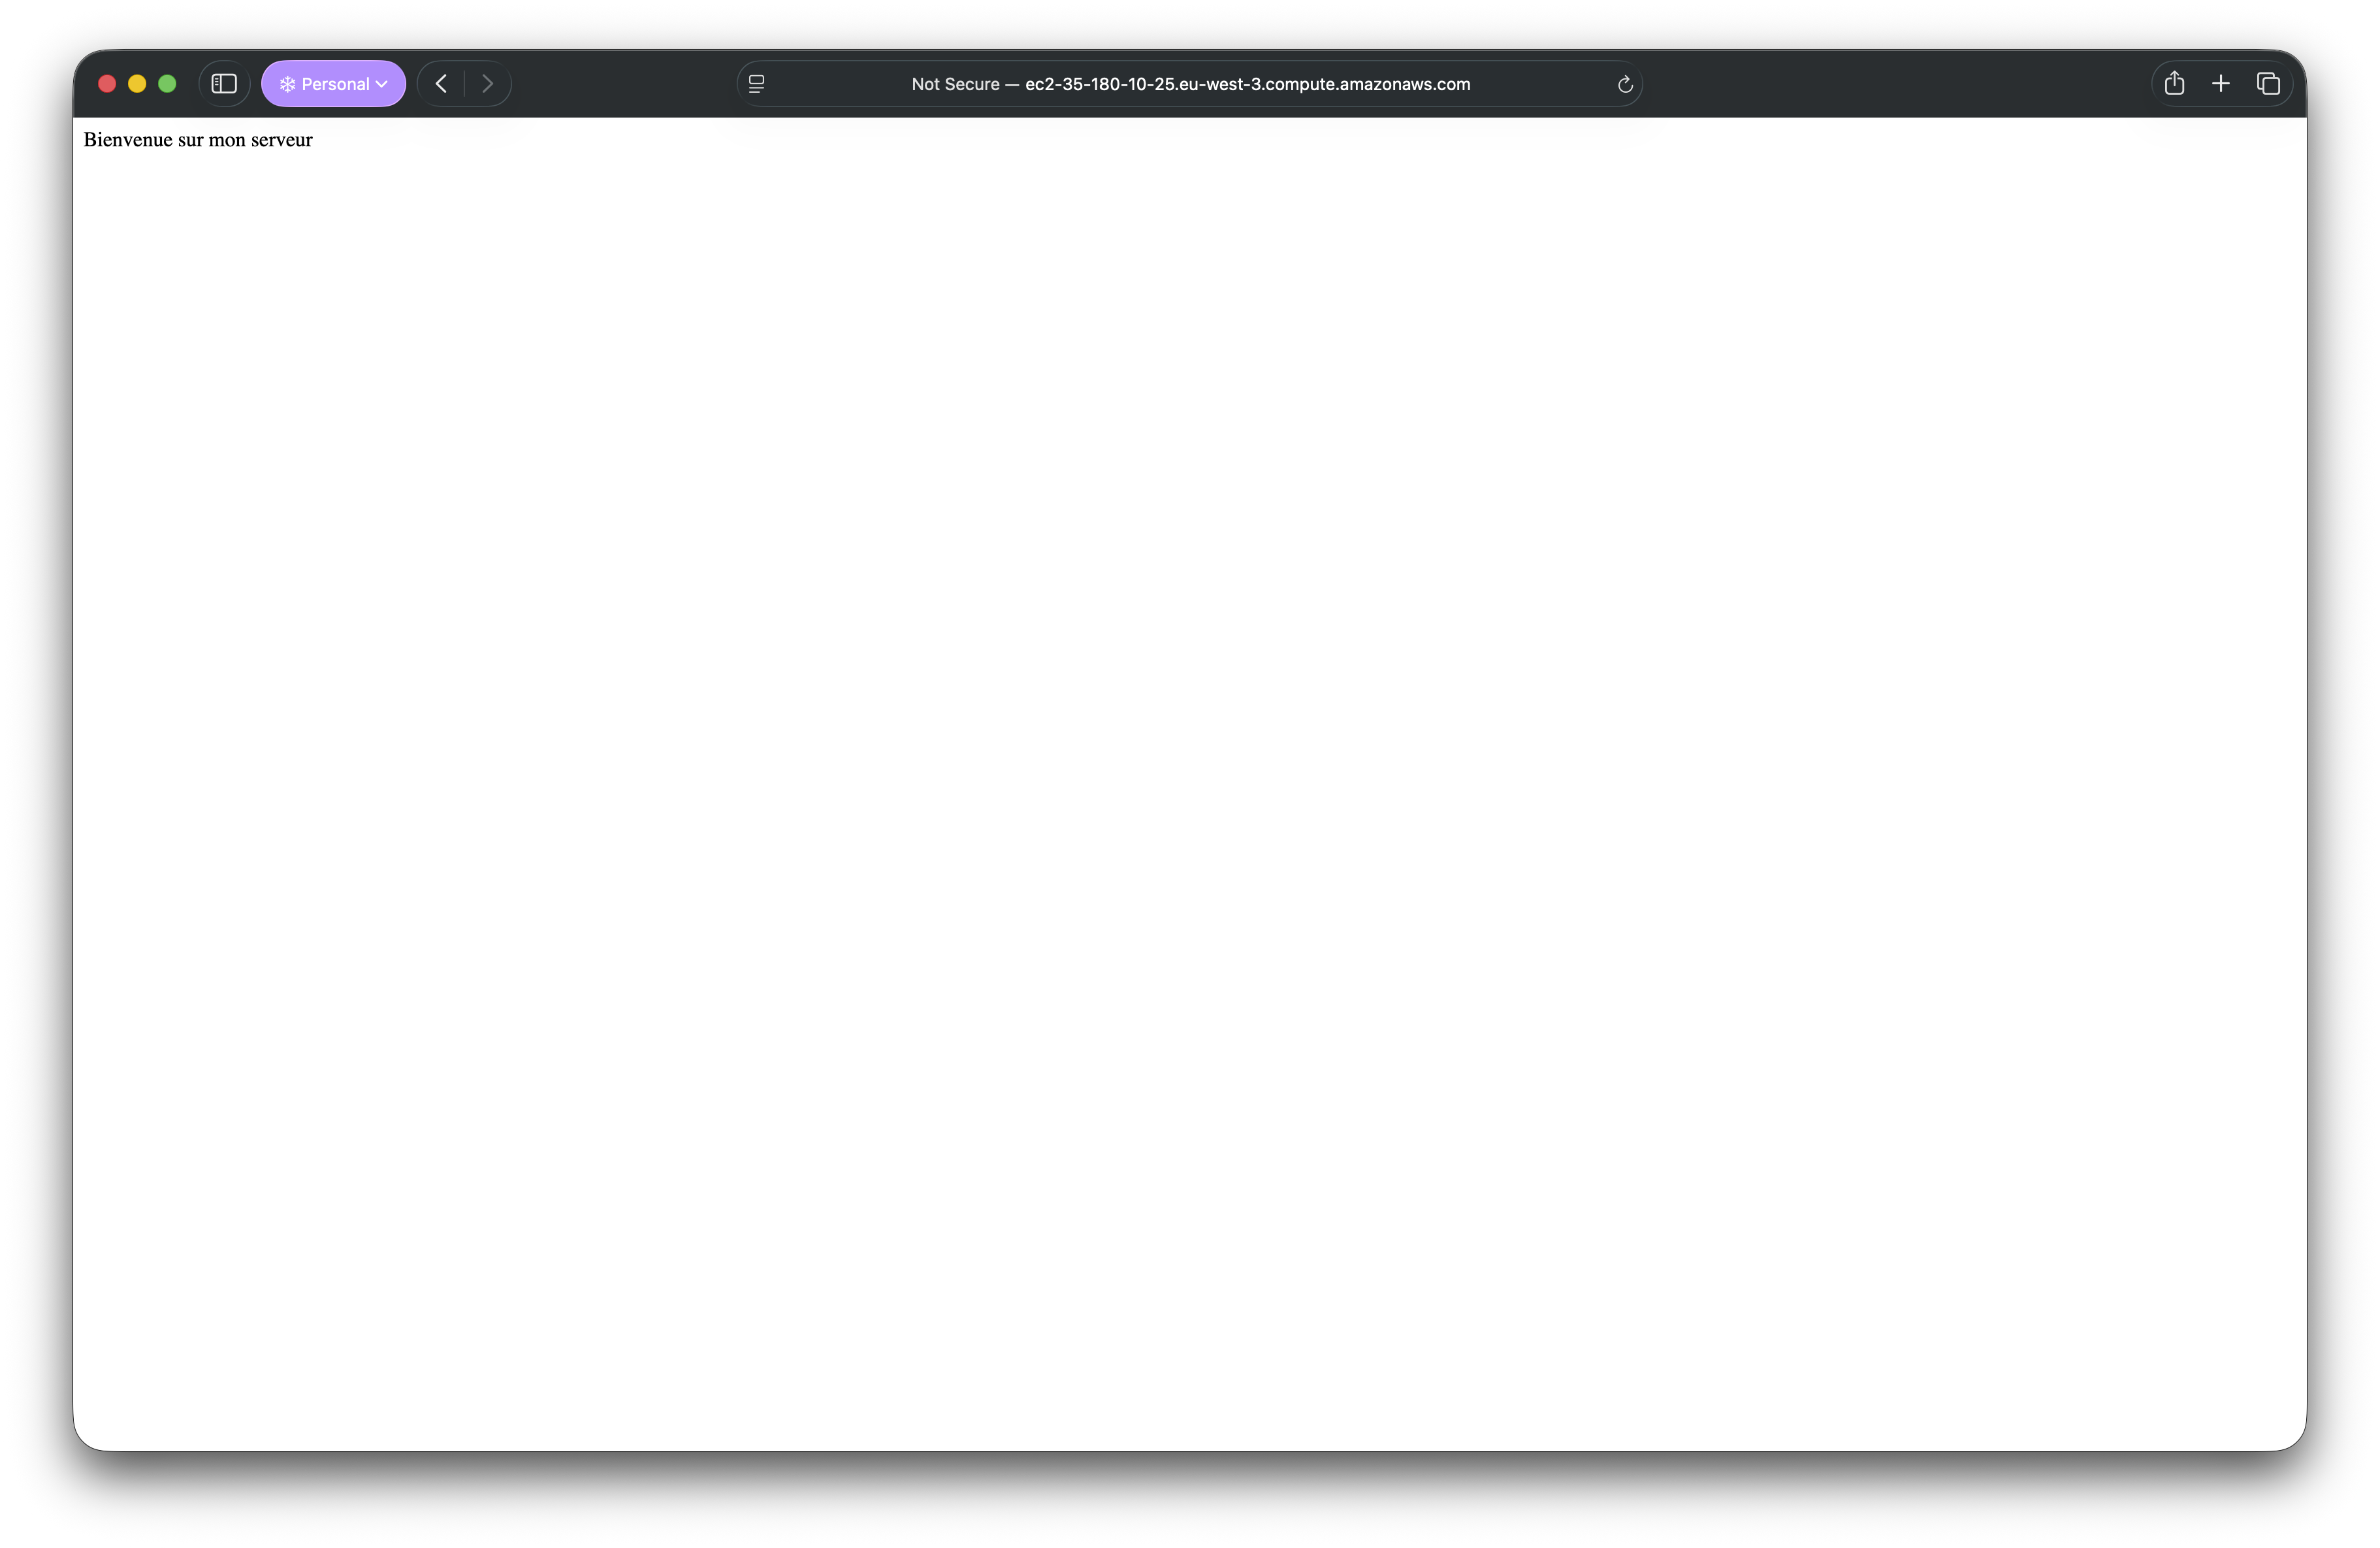
\includegraphics[width=0.65\textwidth]{figures/custom_index_page.png}
    \caption{Custom home page: ``Bienvenue sur mon serveur'' (Arihant Jain)}
\end{figure}

\subsection{Create a DNS Zone with ClouDNS. Give the CNAME and ALIAS Created}
To access our server using a custom domain name instead of the long EC2 public DNS, we set up a free DNS zone on ClouDNS:

\begin{enumerate}
    \item Navigate to \url{https://www.cloudns.net}
    \item Go to \textbf{Create a Zone} $\rightarrow$ \textbf{Free Zone}
    \item Choose the name \texttt{arihant-dev-sail} with the suffix \texttt{.cloud-ip.cc}
\end{enumerate}

We then created the following DNS records:

\begin{itemize}
    \item \textbf{CNAME record:}
    \texttt{arihant-dev-sail.cloud-ip.cc} $\rightarrow$ \texttt{ec2-35-180-10-25.eu-west-3.compute.amazonaws.com}
    \item \textbf{A record (ALIAS):}
    \texttt{arihant-dev-sail.cloud-ip.cc} $\rightarrow$ \texttt{35.180.10.25}
\end{itemize}

\begin{figure}[H]
    \centering
    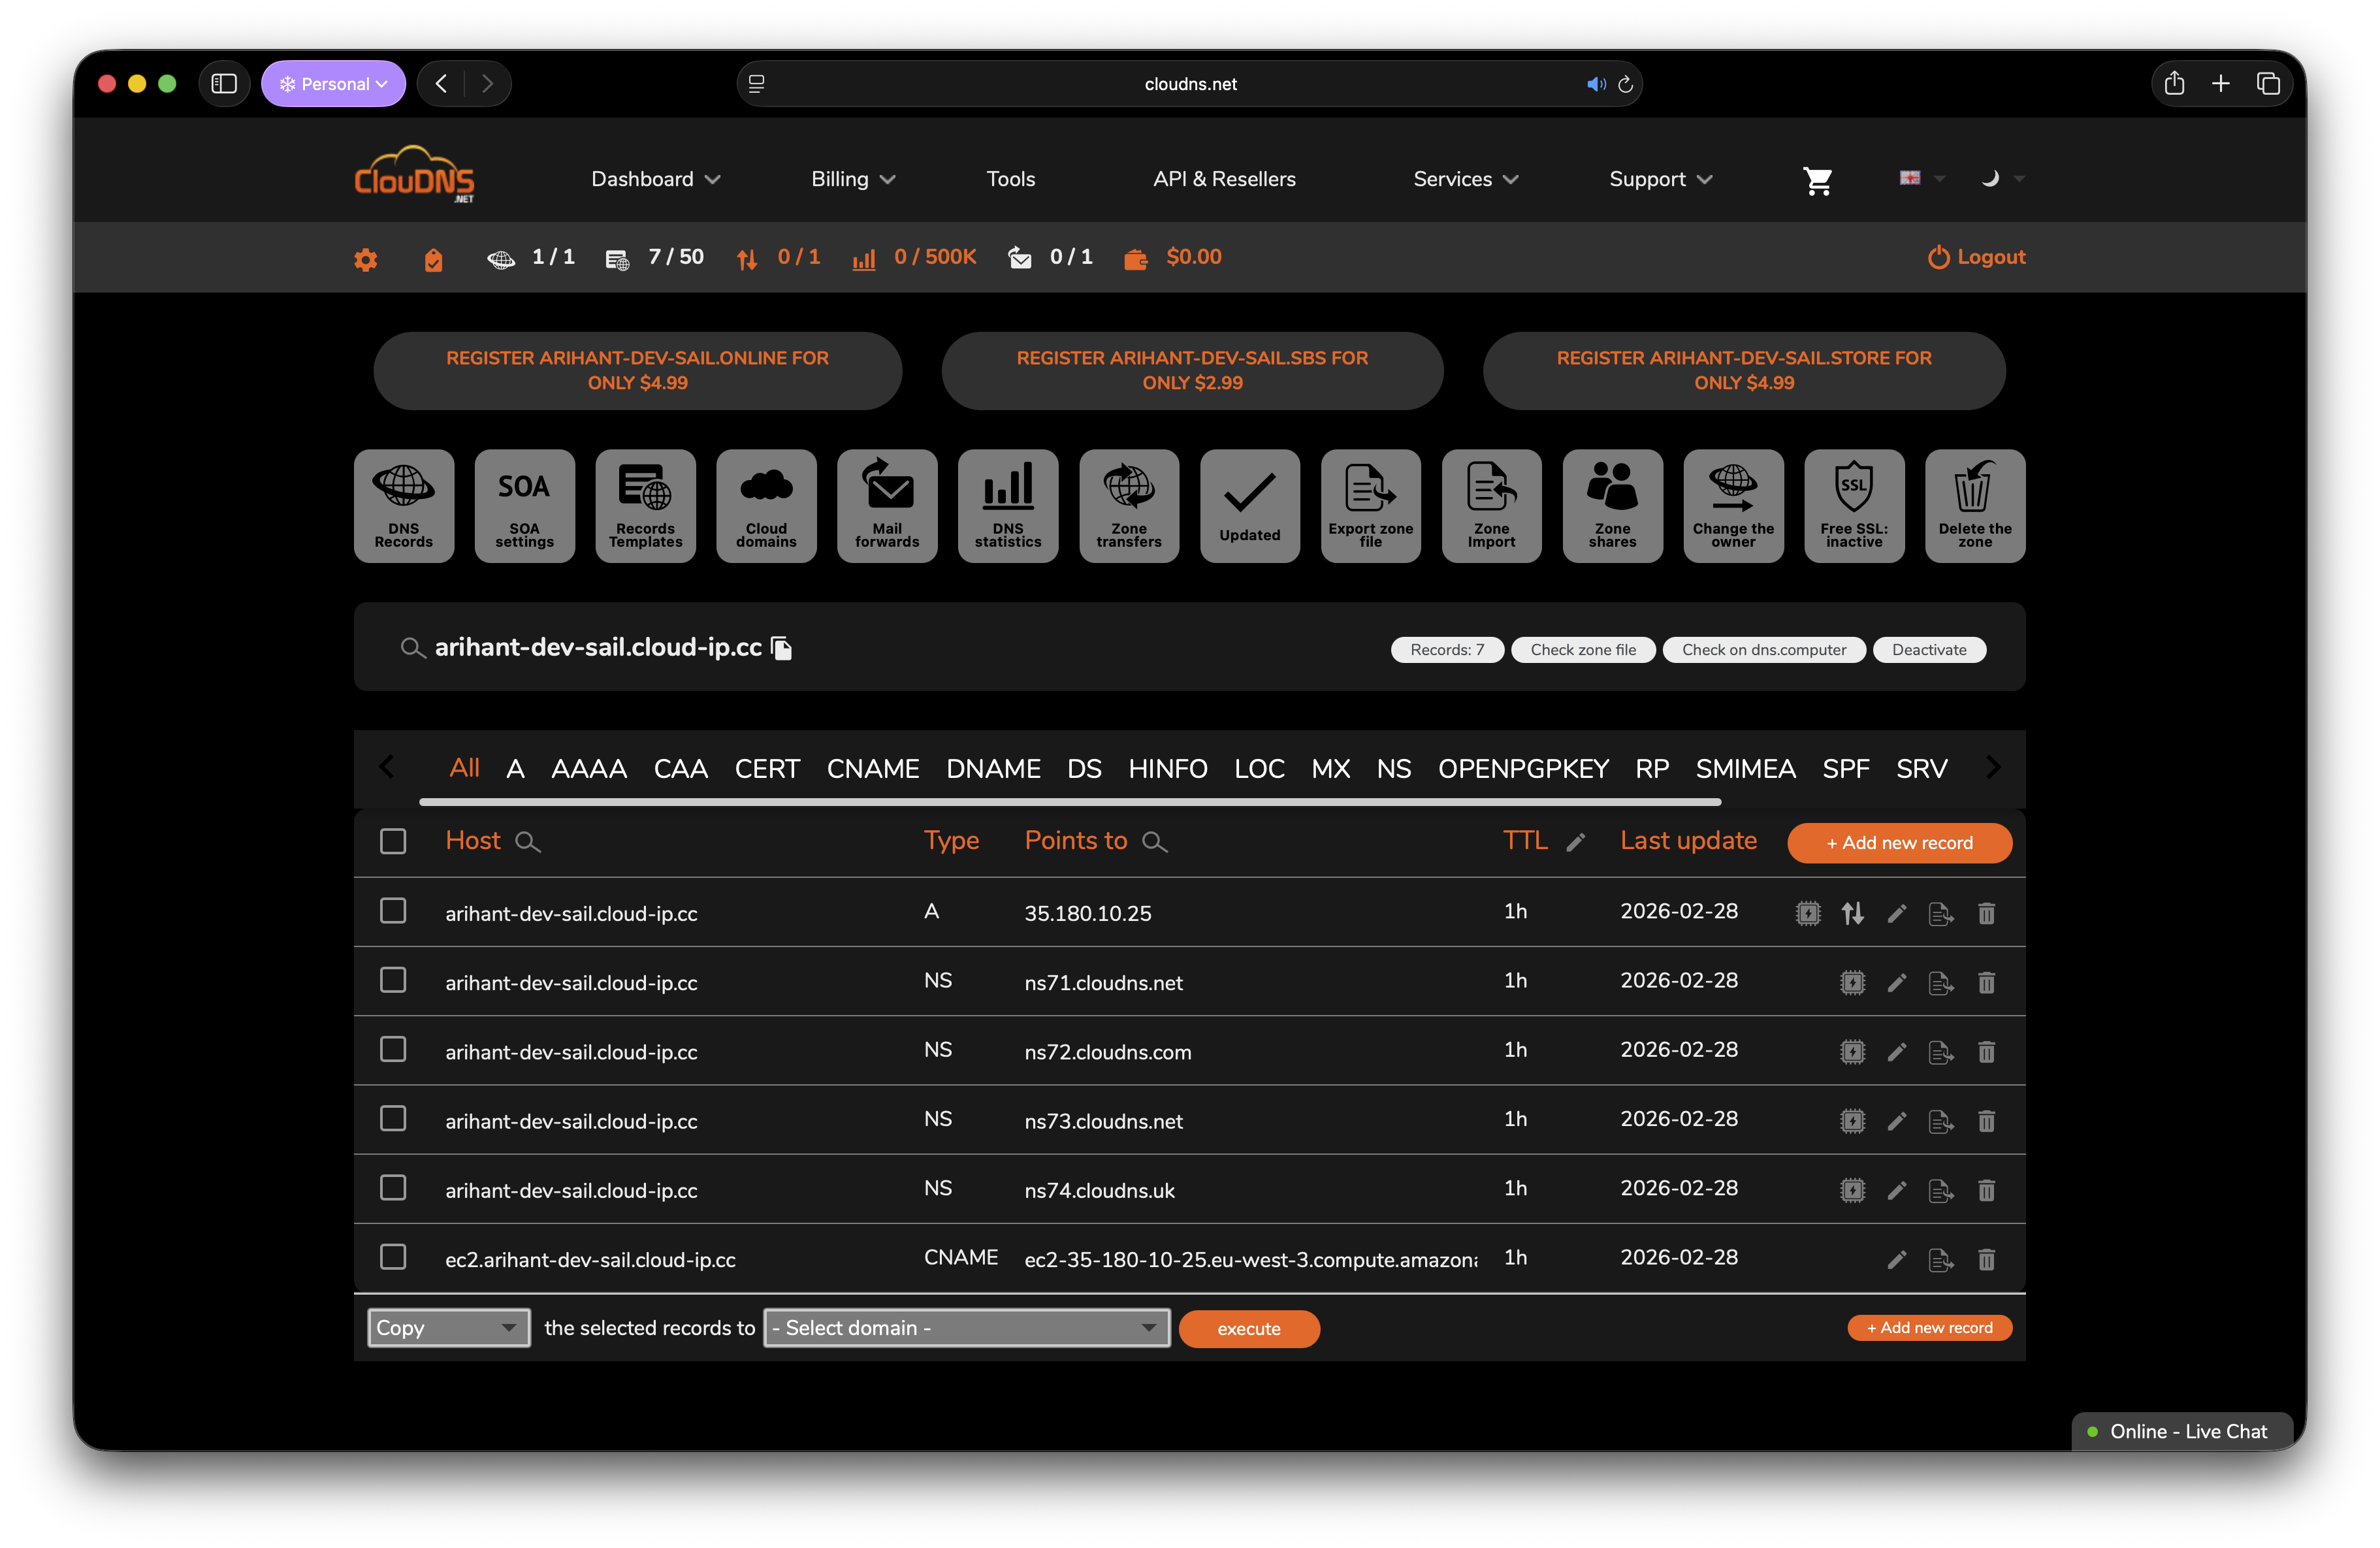
\includegraphics[width=0.65\textwidth]{figures/cloudns.png}
    \caption{ClouDNS zone configuration with CNAME and A record (Arihant Jain)}
\end{figure}

\subsection{Check DNS Resolution with the dig Command}
After DNS propagation, we verify that the domain resolves correctly using the \texttt{dig} command:

\begin{lstlisting}[language=bash]
dig +short ec2.arihant-dev-sail.cloud-ip.cc
\end{lstlisting}

The output confirms the A record resolving to our EC2 public IPv4 address \texttt{35.180.10.25}, confirming that the DNS zone is properly configured.

\begin{figure}[H]
    \centering
    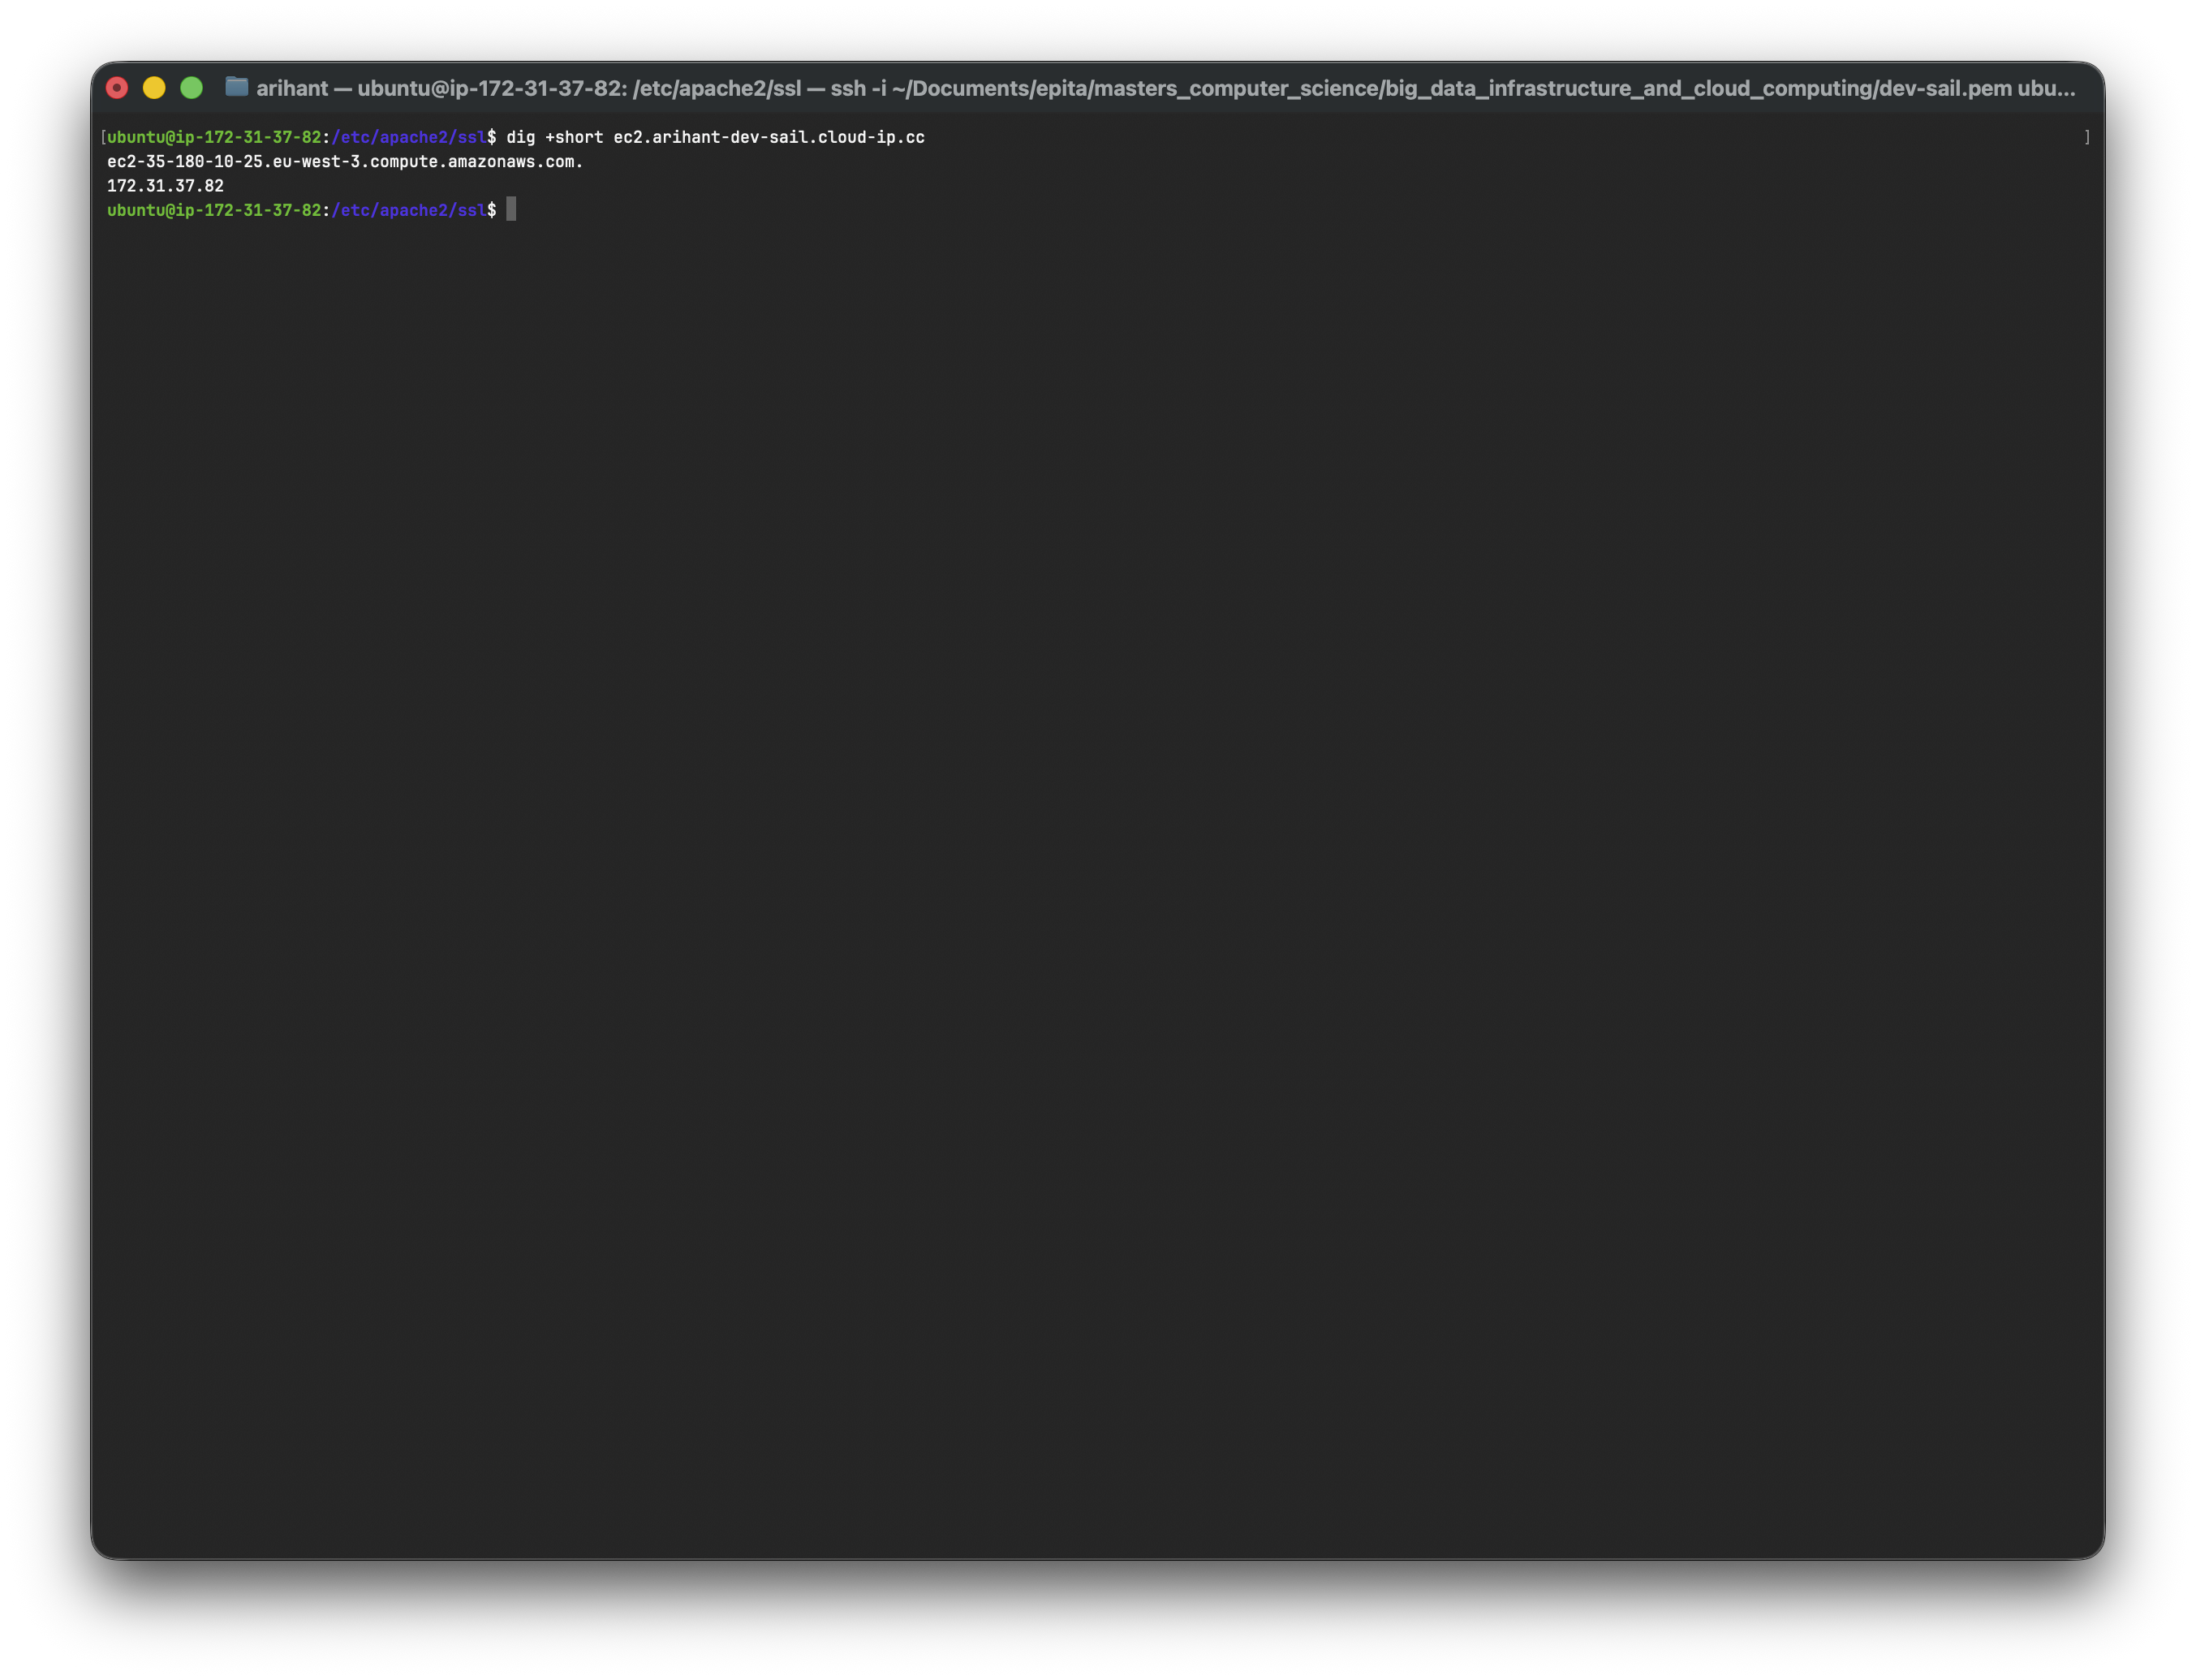
\includegraphics[width=0.65\textwidth]{figures/dig_output.png}
    \caption{DNS resolution verified with dig (Arihant Jain)}
\end{figure}

\subsection{Test with a Web Browser}
After DNS propagation, the server is now accessible via our custom domain at:

\begin{center}
\texttt{http://arihant-dev-sail.cloud-ip.cc}
\end{center}

The browser displays our custom ``Bienvenue sur mon serveur'' page, confirming that the DNS is correctly pointing to our EC2 instance. However, the connection is not secured --- the site is served over plain HTTP, as shown by the browser warning.

\begin{figure}[H]
    \centering
    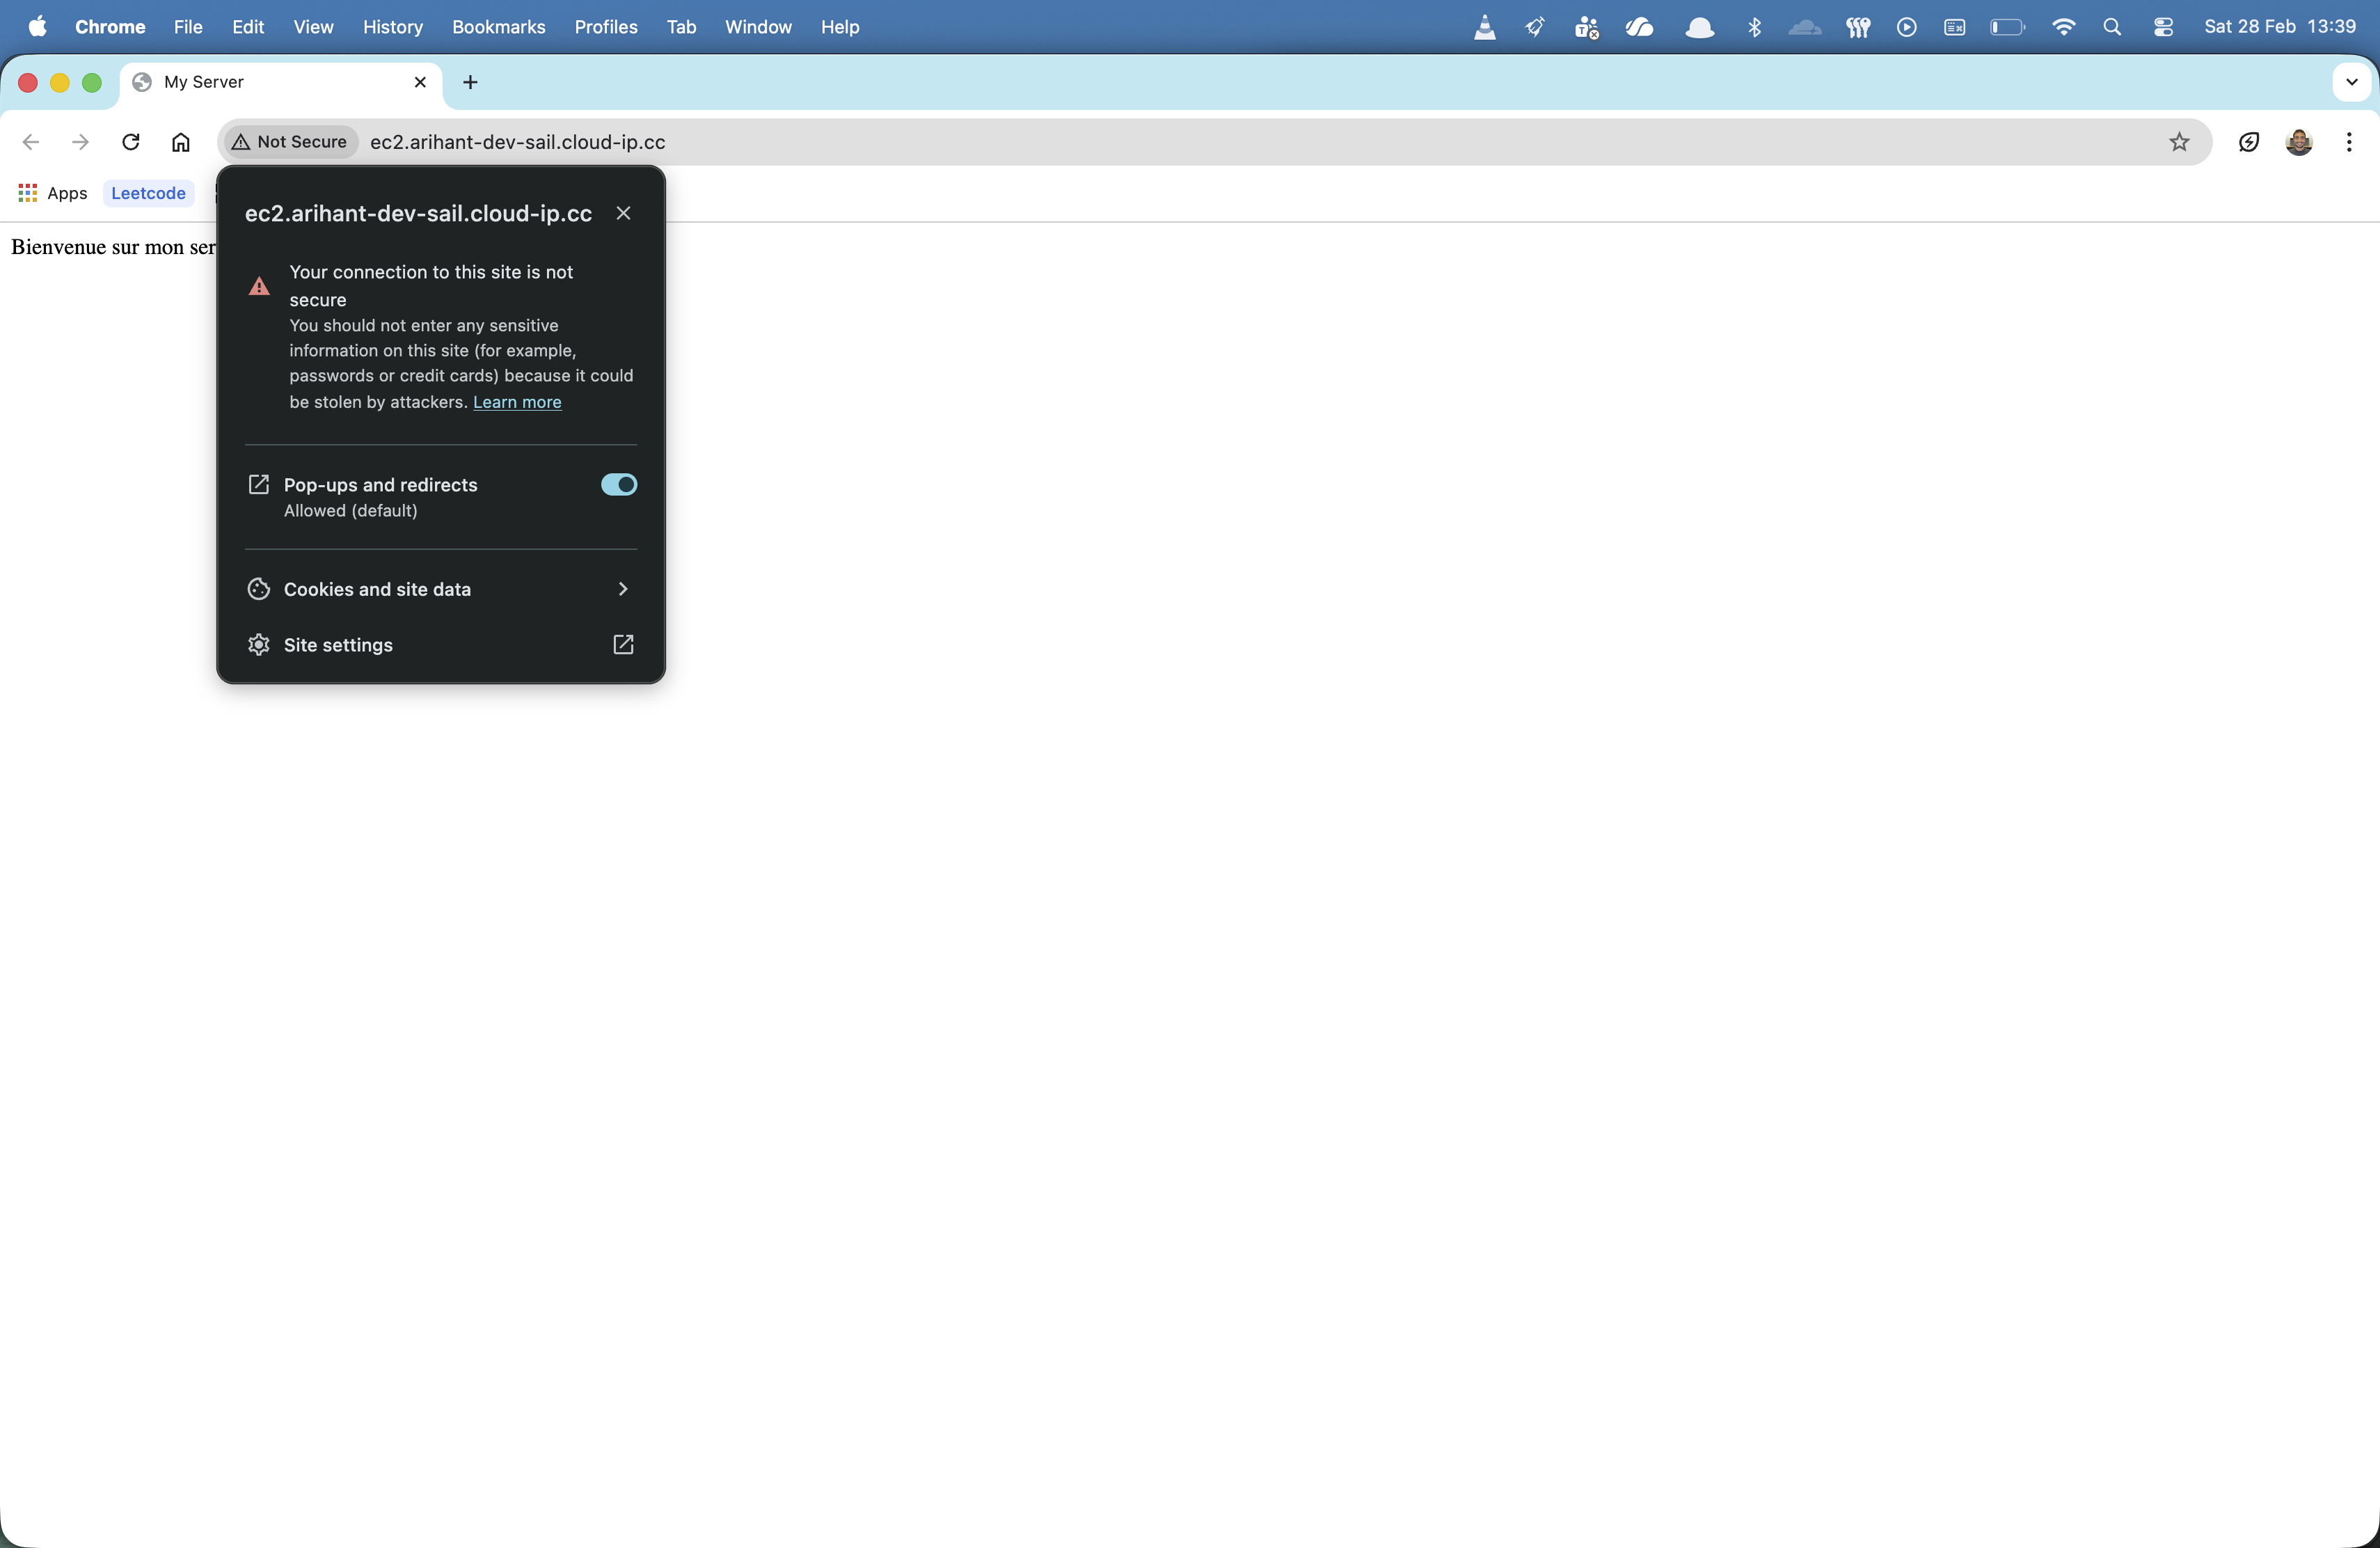
\includegraphics[width=0.65\textwidth]{figures/self_signed_certificate_webpage.png}
    \caption{Site accessible via custom domain over HTTP (Arihant Jain)}
\end{figure}

\subsection{Create and Install a Self-Signed Certificate. Test with a Web Browser}
As a first step toward securing the site, we generated a self-signed SSL certificate. We enabled the SSL module in Apache and configured it:

\begin{lstlisting}[language=bash]
sudo a2enmod ssl
sudo openssl req -x509 -nodes -days 365 -newkey rsa:2048 \
    -keyout /etc/ssl/private/apache-selfsigned.key \
    -out /etc/ssl/certs/apache-selfsigned.crt
sudo systemctl restart apache2
\end{lstlisting}

\begin{figure}[H]
    \centering
    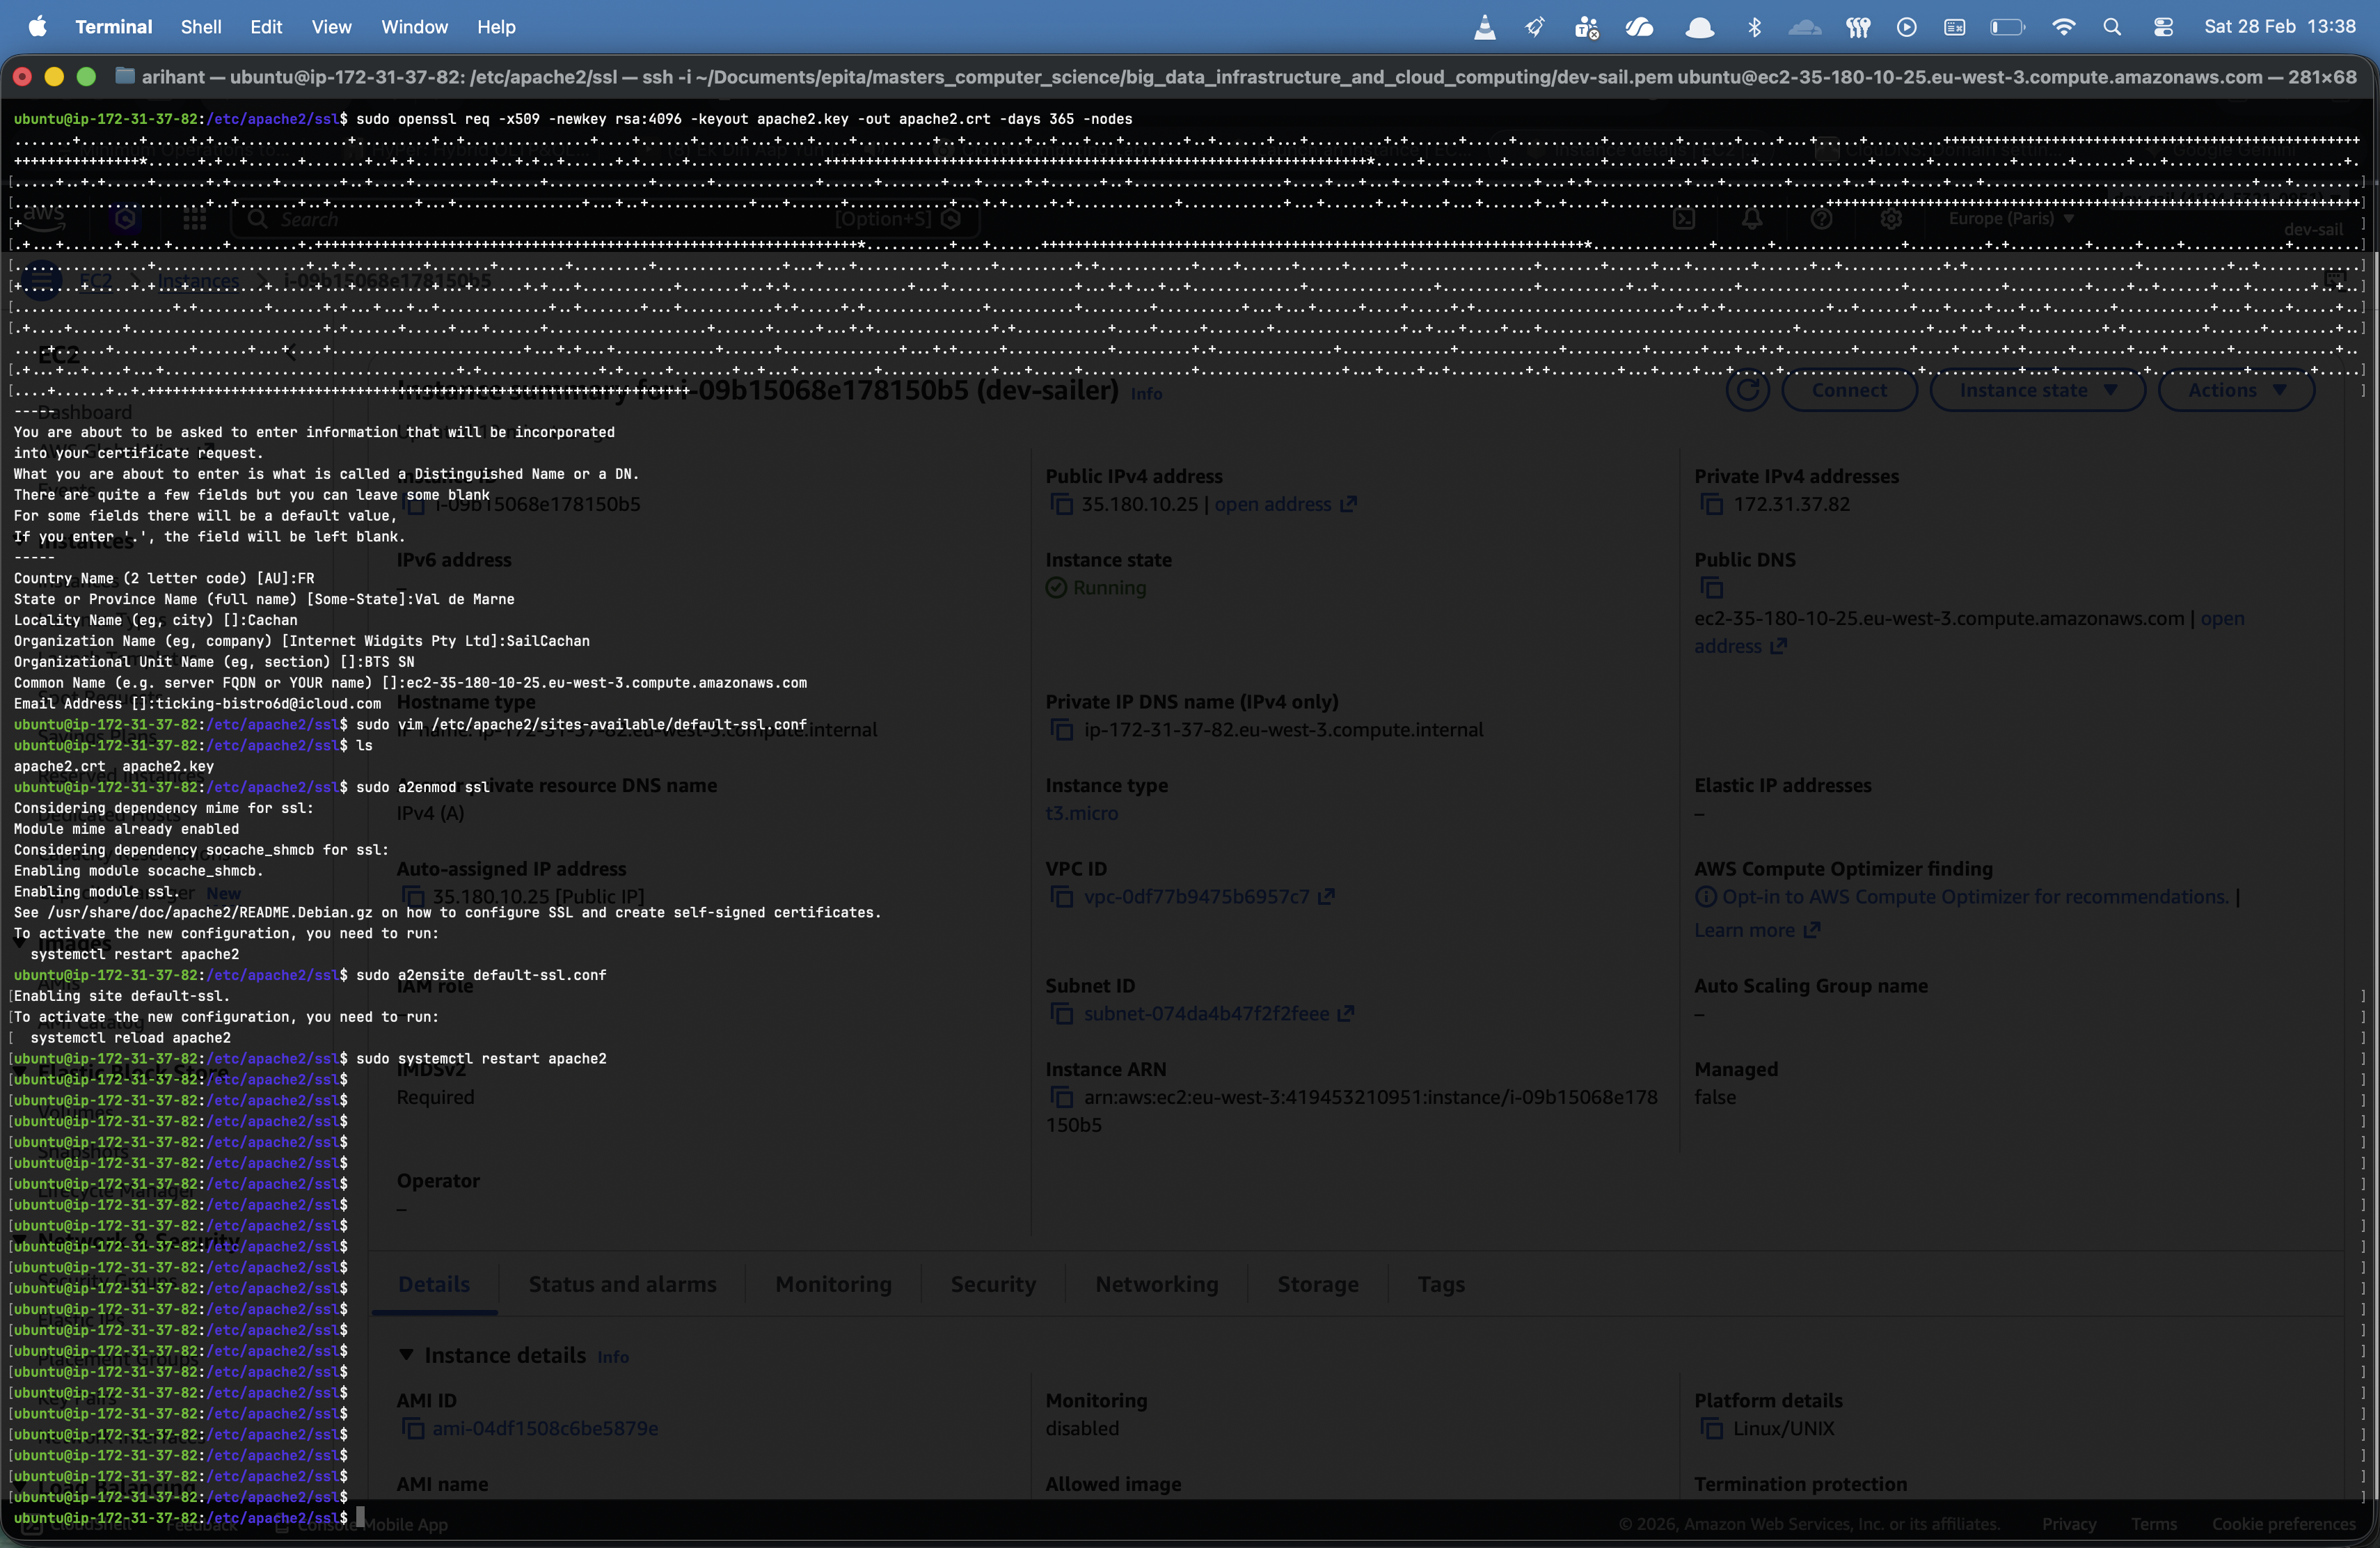
\includegraphics[width=0.65\textwidth]{figures/self_signed_certificate_cmd.png}
    \caption{Generating a self-signed SSL certificate (Arihant Jain)}
\end{figure}

While this enables HTTPS, the browser displays a security warning because the certificate is not issued by a trusted Certificate Authority (CA). The connection is encrypted, but the browser cannot verify the server's identity.

\begin{figure}[H]
    \centering
    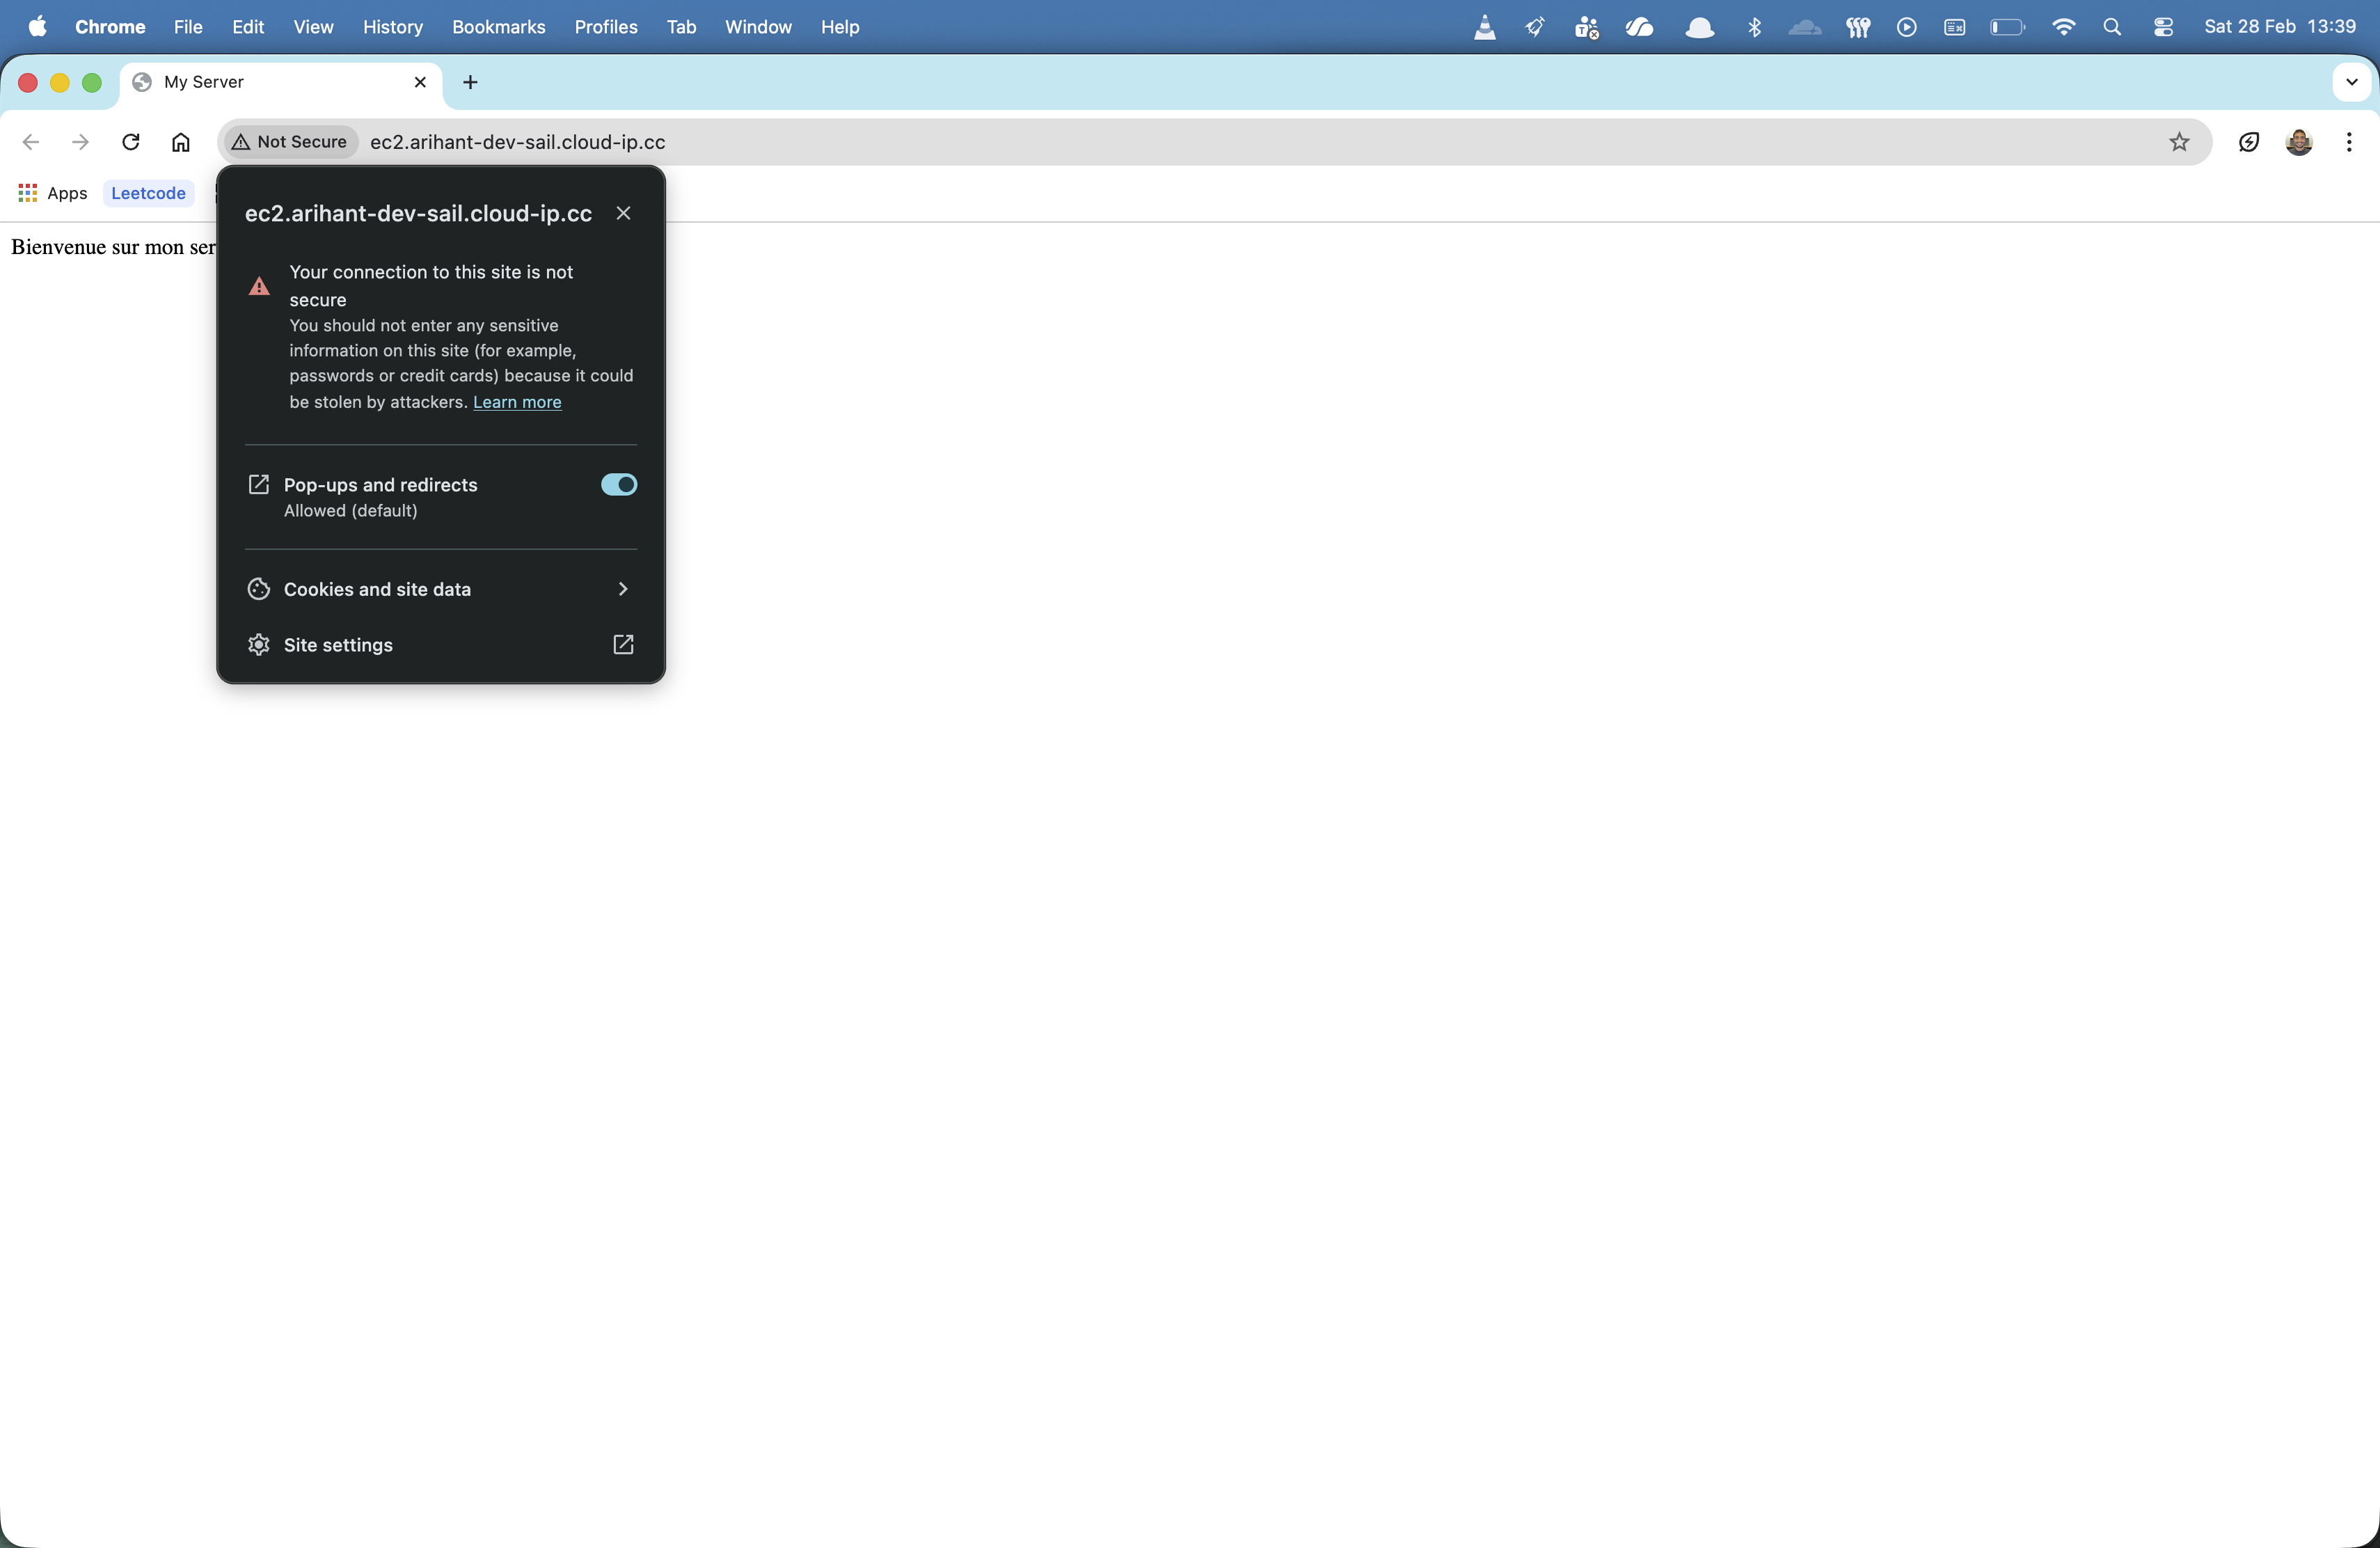
\includegraphics[width=0.65\textwidth]{figures/self_signed_certificate_webpage.png}
    \caption{Browser warning for self-signed certificate (Arihant Jain)}
\end{figure}

\subsection{Create and Install a Certified Certificate with ZeroSSL. Test with a Web Browser}
To get a ZeroSSL certificate, we need to register an account on ZeroSSL and request the certificate on the website.
After that, we need to use CNAME verification to ensu we can install our certificate by adding the url for verification to our DNS Zone.
\begin{figure}[H]
    \centering
    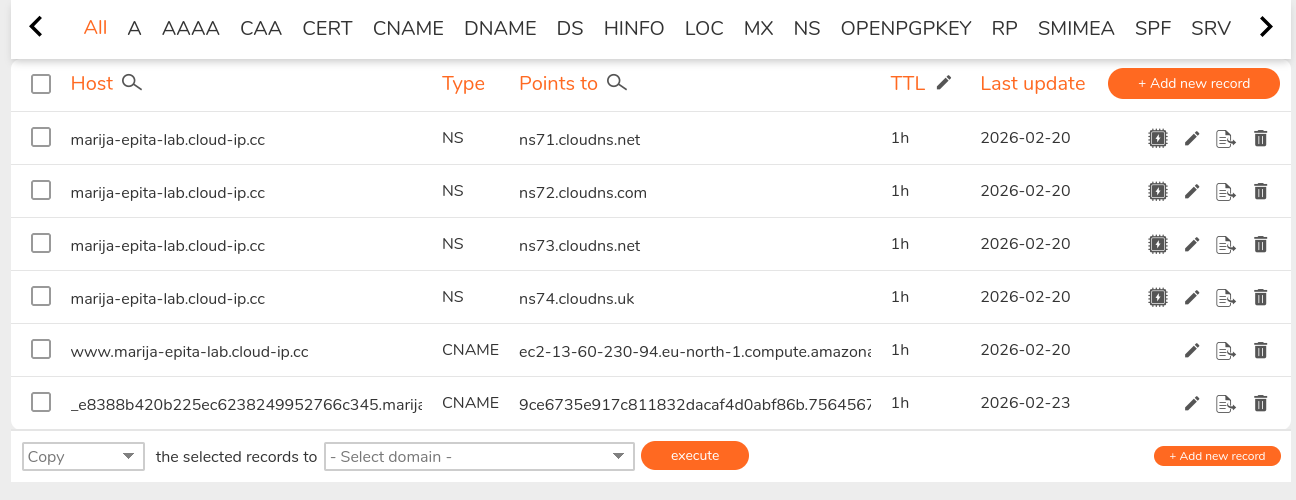
\includegraphics[width=0.65\textwidth]{figures/cnameverification.png}
    \caption{CName verification setting on DNS Zone (Huizhe Su)}
\end{figure}
Then we need to download and upload the certificate to our server, with following configuration.
We use \texttt{scp} to upload the files to our remote instance.
\begin{lstlisting}[language=bash]
scp ./www.marija-epita-lab.cloud-ip.cc.zip aws_epita:/home/ubuntu
\end{lstlisting}
Then we will unzip it and install them into \texttt{/etc/apache2/ssl/}
\begin{figure}[H]
    \centering
    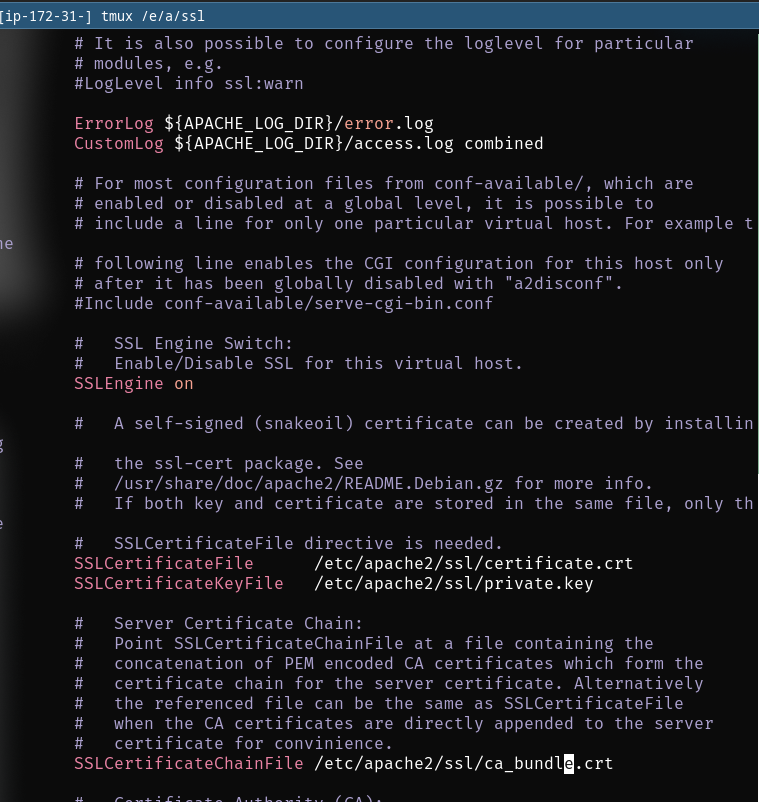
\includegraphics[width=0.65\textwidth]{figures/zerosslconfig.png}
    \caption{ZeroSSL configuration (Huizhe Su)}
\end{figure}
Then, we restart apache service.
\begin{lstlisting}[language=bash]
sudo systemctl restart apache2
\end{lstlisting}
Then we can verify the installation on ZeroSSL website.
\begin{figure}[H]
    \centering
    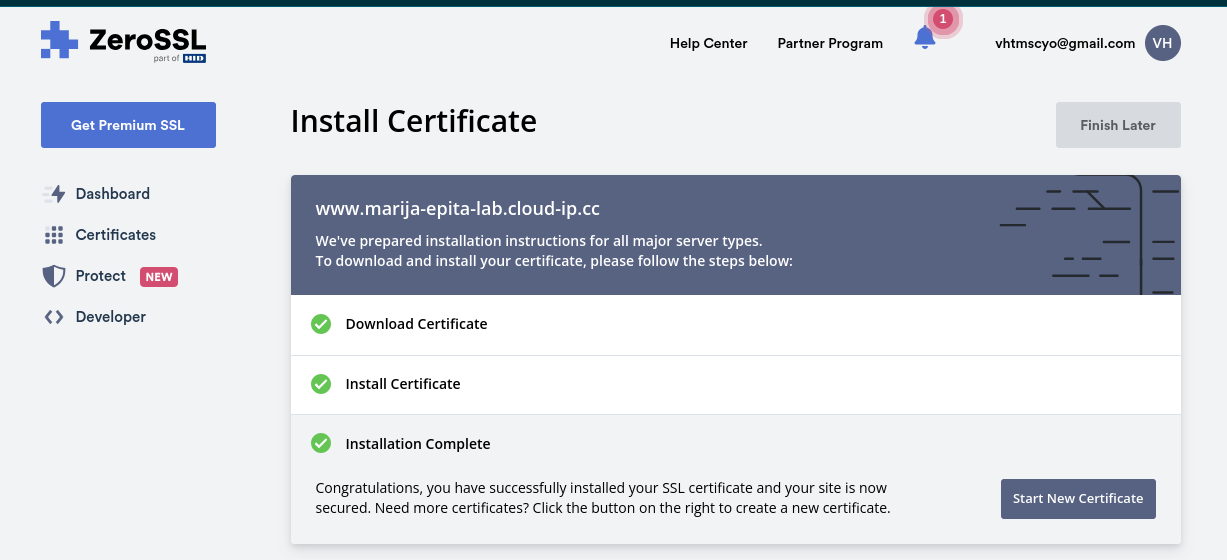
\includegraphics[width=0.65\textwidth]{figures/zerosslverification.png}
    \caption{Verification result on ZeroSSL (Huizhe Su)}
\end{figure}
Now when we can go to our website \url{www.marija-epita-lab.cloud-ip.cc}, we can see the certificate is ZeroSSL.
\begin{figure}[H]
    \centering
    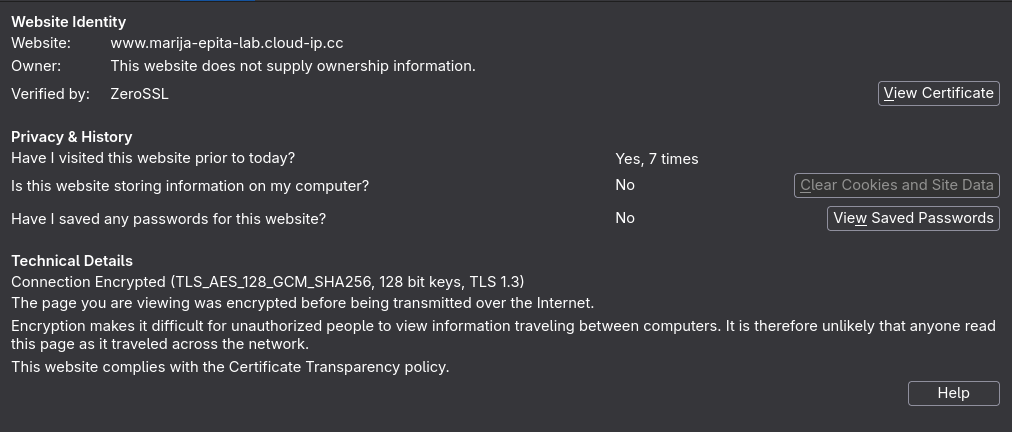
\includegraphics[width=0.65\textwidth]{figures/zerossl.png}
    \caption{ZeroSSL certificate (Huizhe Su)}
\end{figure}
\subsection{Create and Install a Certified Certificate with Let's Encrypt and Certbot. Test with a Web Browser}
To obtain a trusted SSL certificate with automatic renewal, we used Certbot with Let's Encrypt. First, we install Certbot and its Apache plugin:

\begin{lstlisting}[language=bash]
sudo apt install certbot python3-certbot-apache
\end{lstlisting}

Then we request a free SSL certificate for our domain:

\begin{lstlisting}[language=bash]
sudo certbot --apache -d arihant-dev-sail.cloud-ip.cc
\end{lstlisting}

Certbot automatically configures Apache to use the new certificate.

\begin{figure}[H]
    \centering
    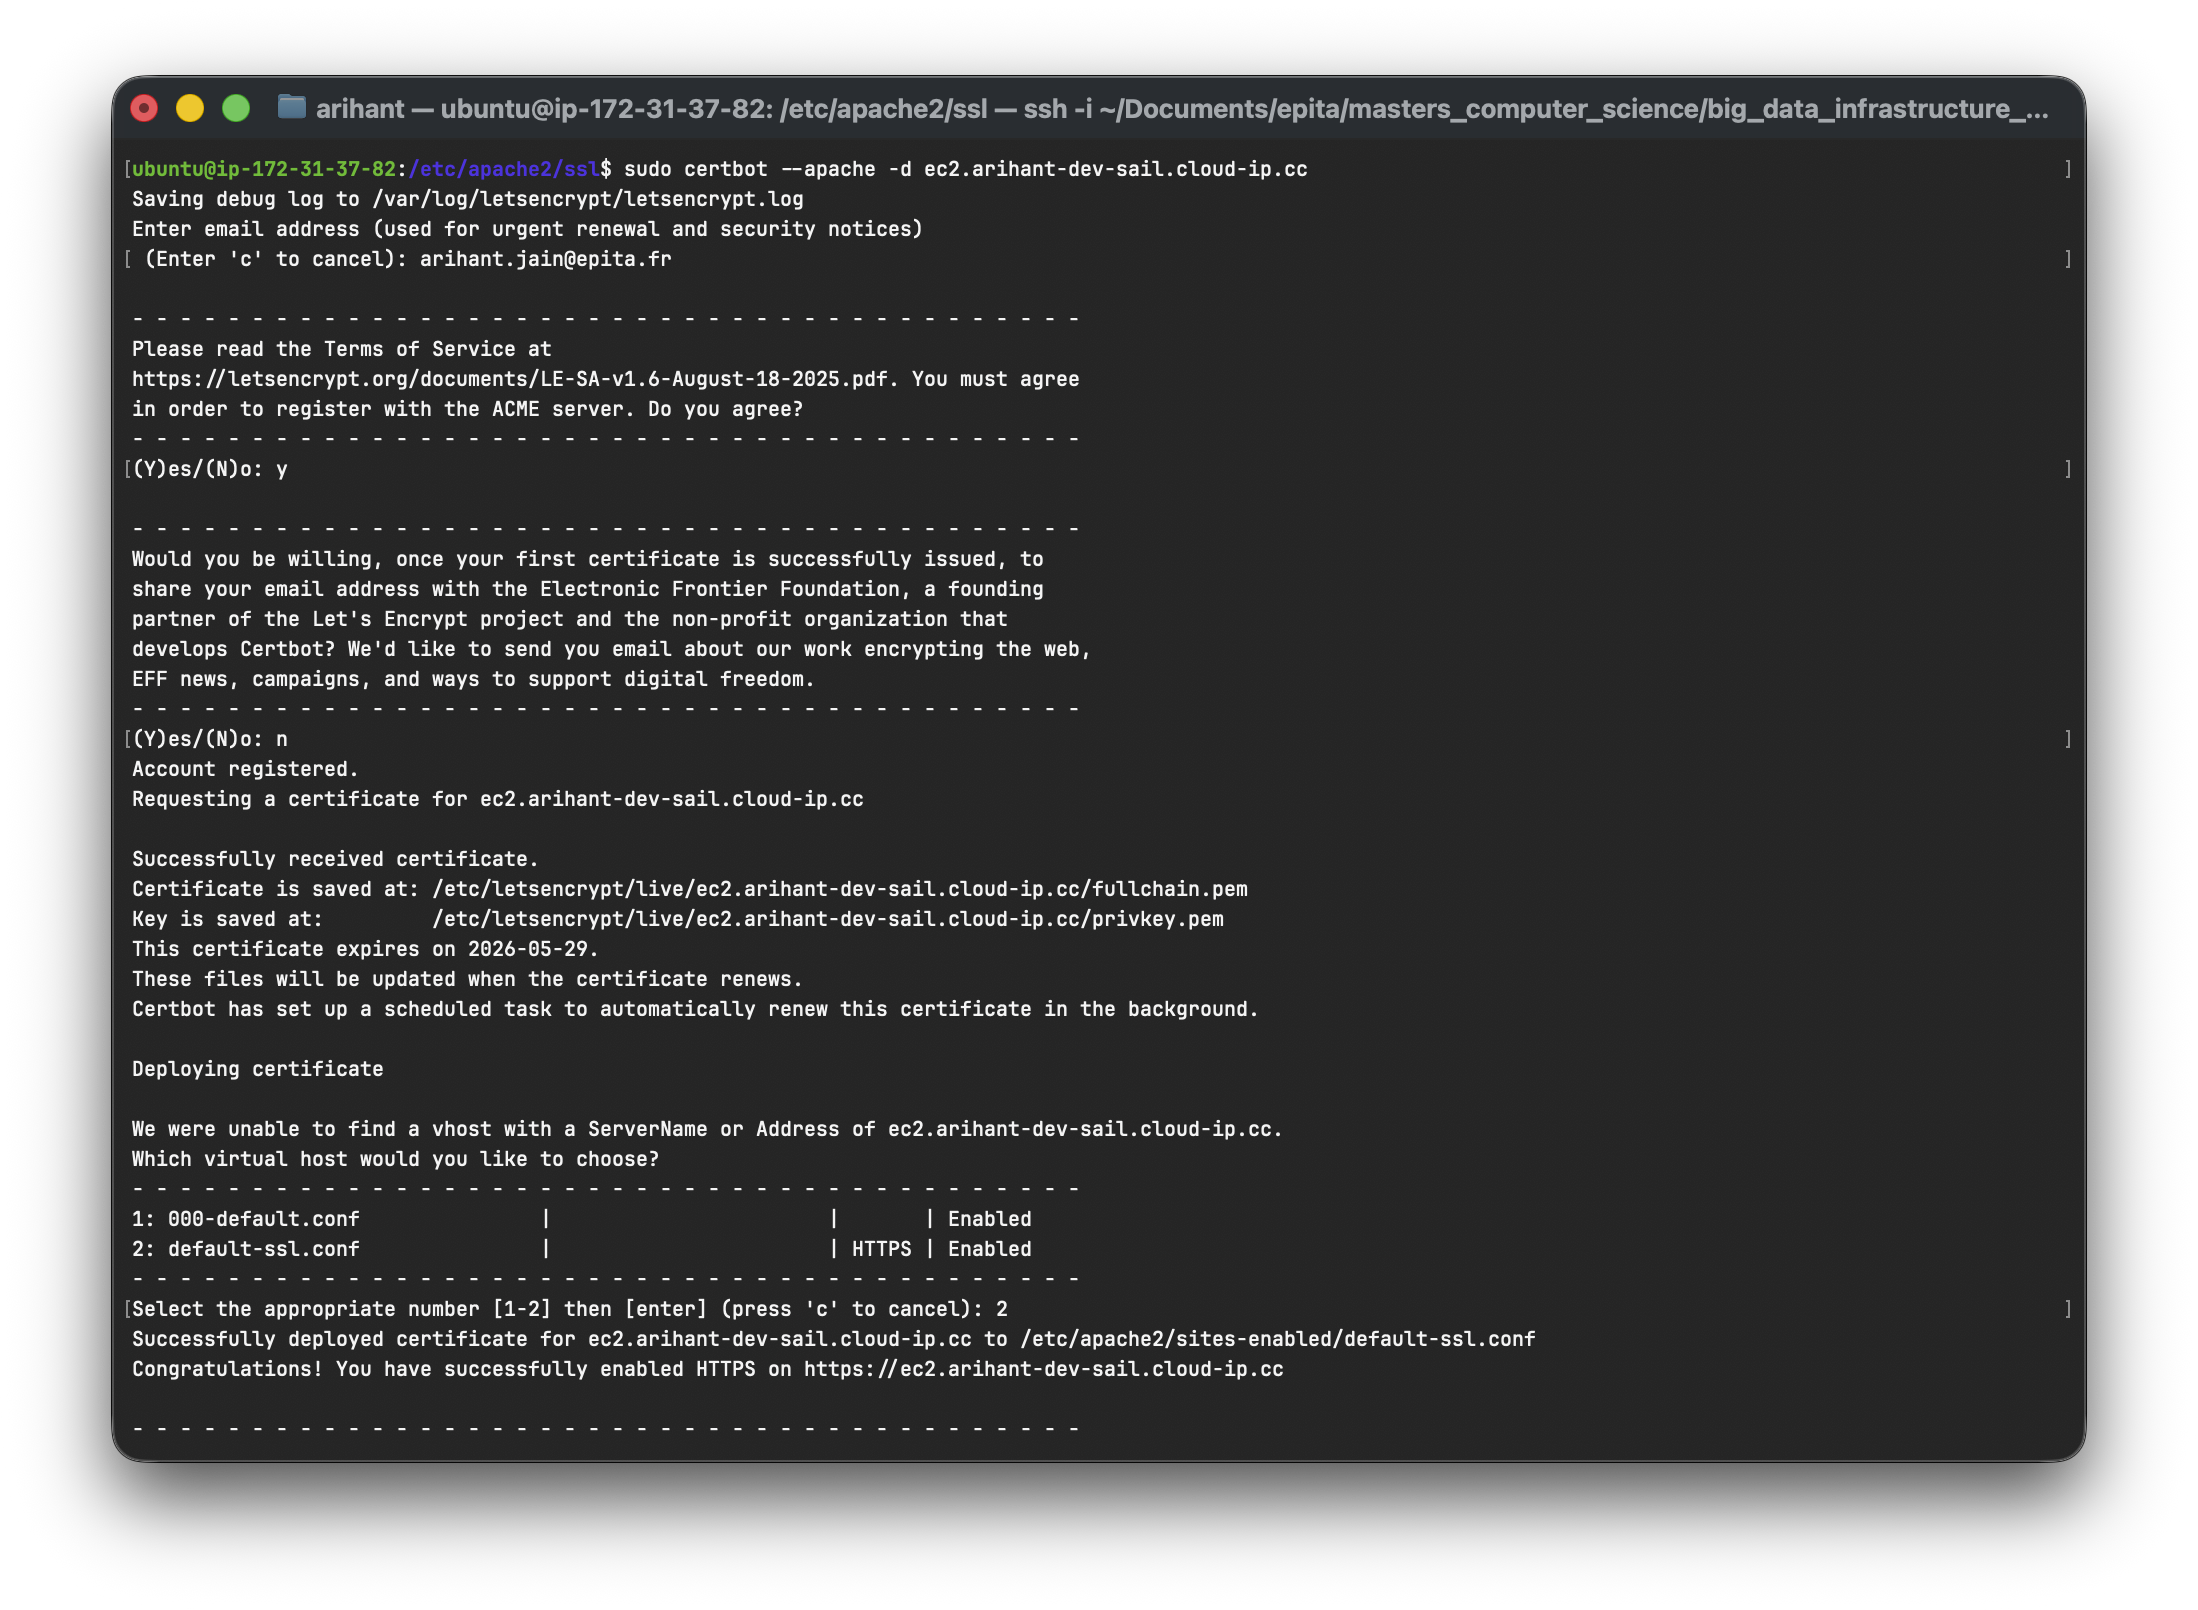
\includegraphics[width=0.65\textwidth]{figures/certbot_certificate.png}
    \caption{Certbot successfully obtaining a Let's Encrypt certificate (Arihant Jain)}
\end{figure}

The site is now accessible securely at \texttt{https://arihant-dev-sail.cloud-ip.cc} with a valid SSL certificate issued by Let's Encrypt. The browser shows a padlock icon confirming the secure connection.

\begin{figure}[H]
    \centering
    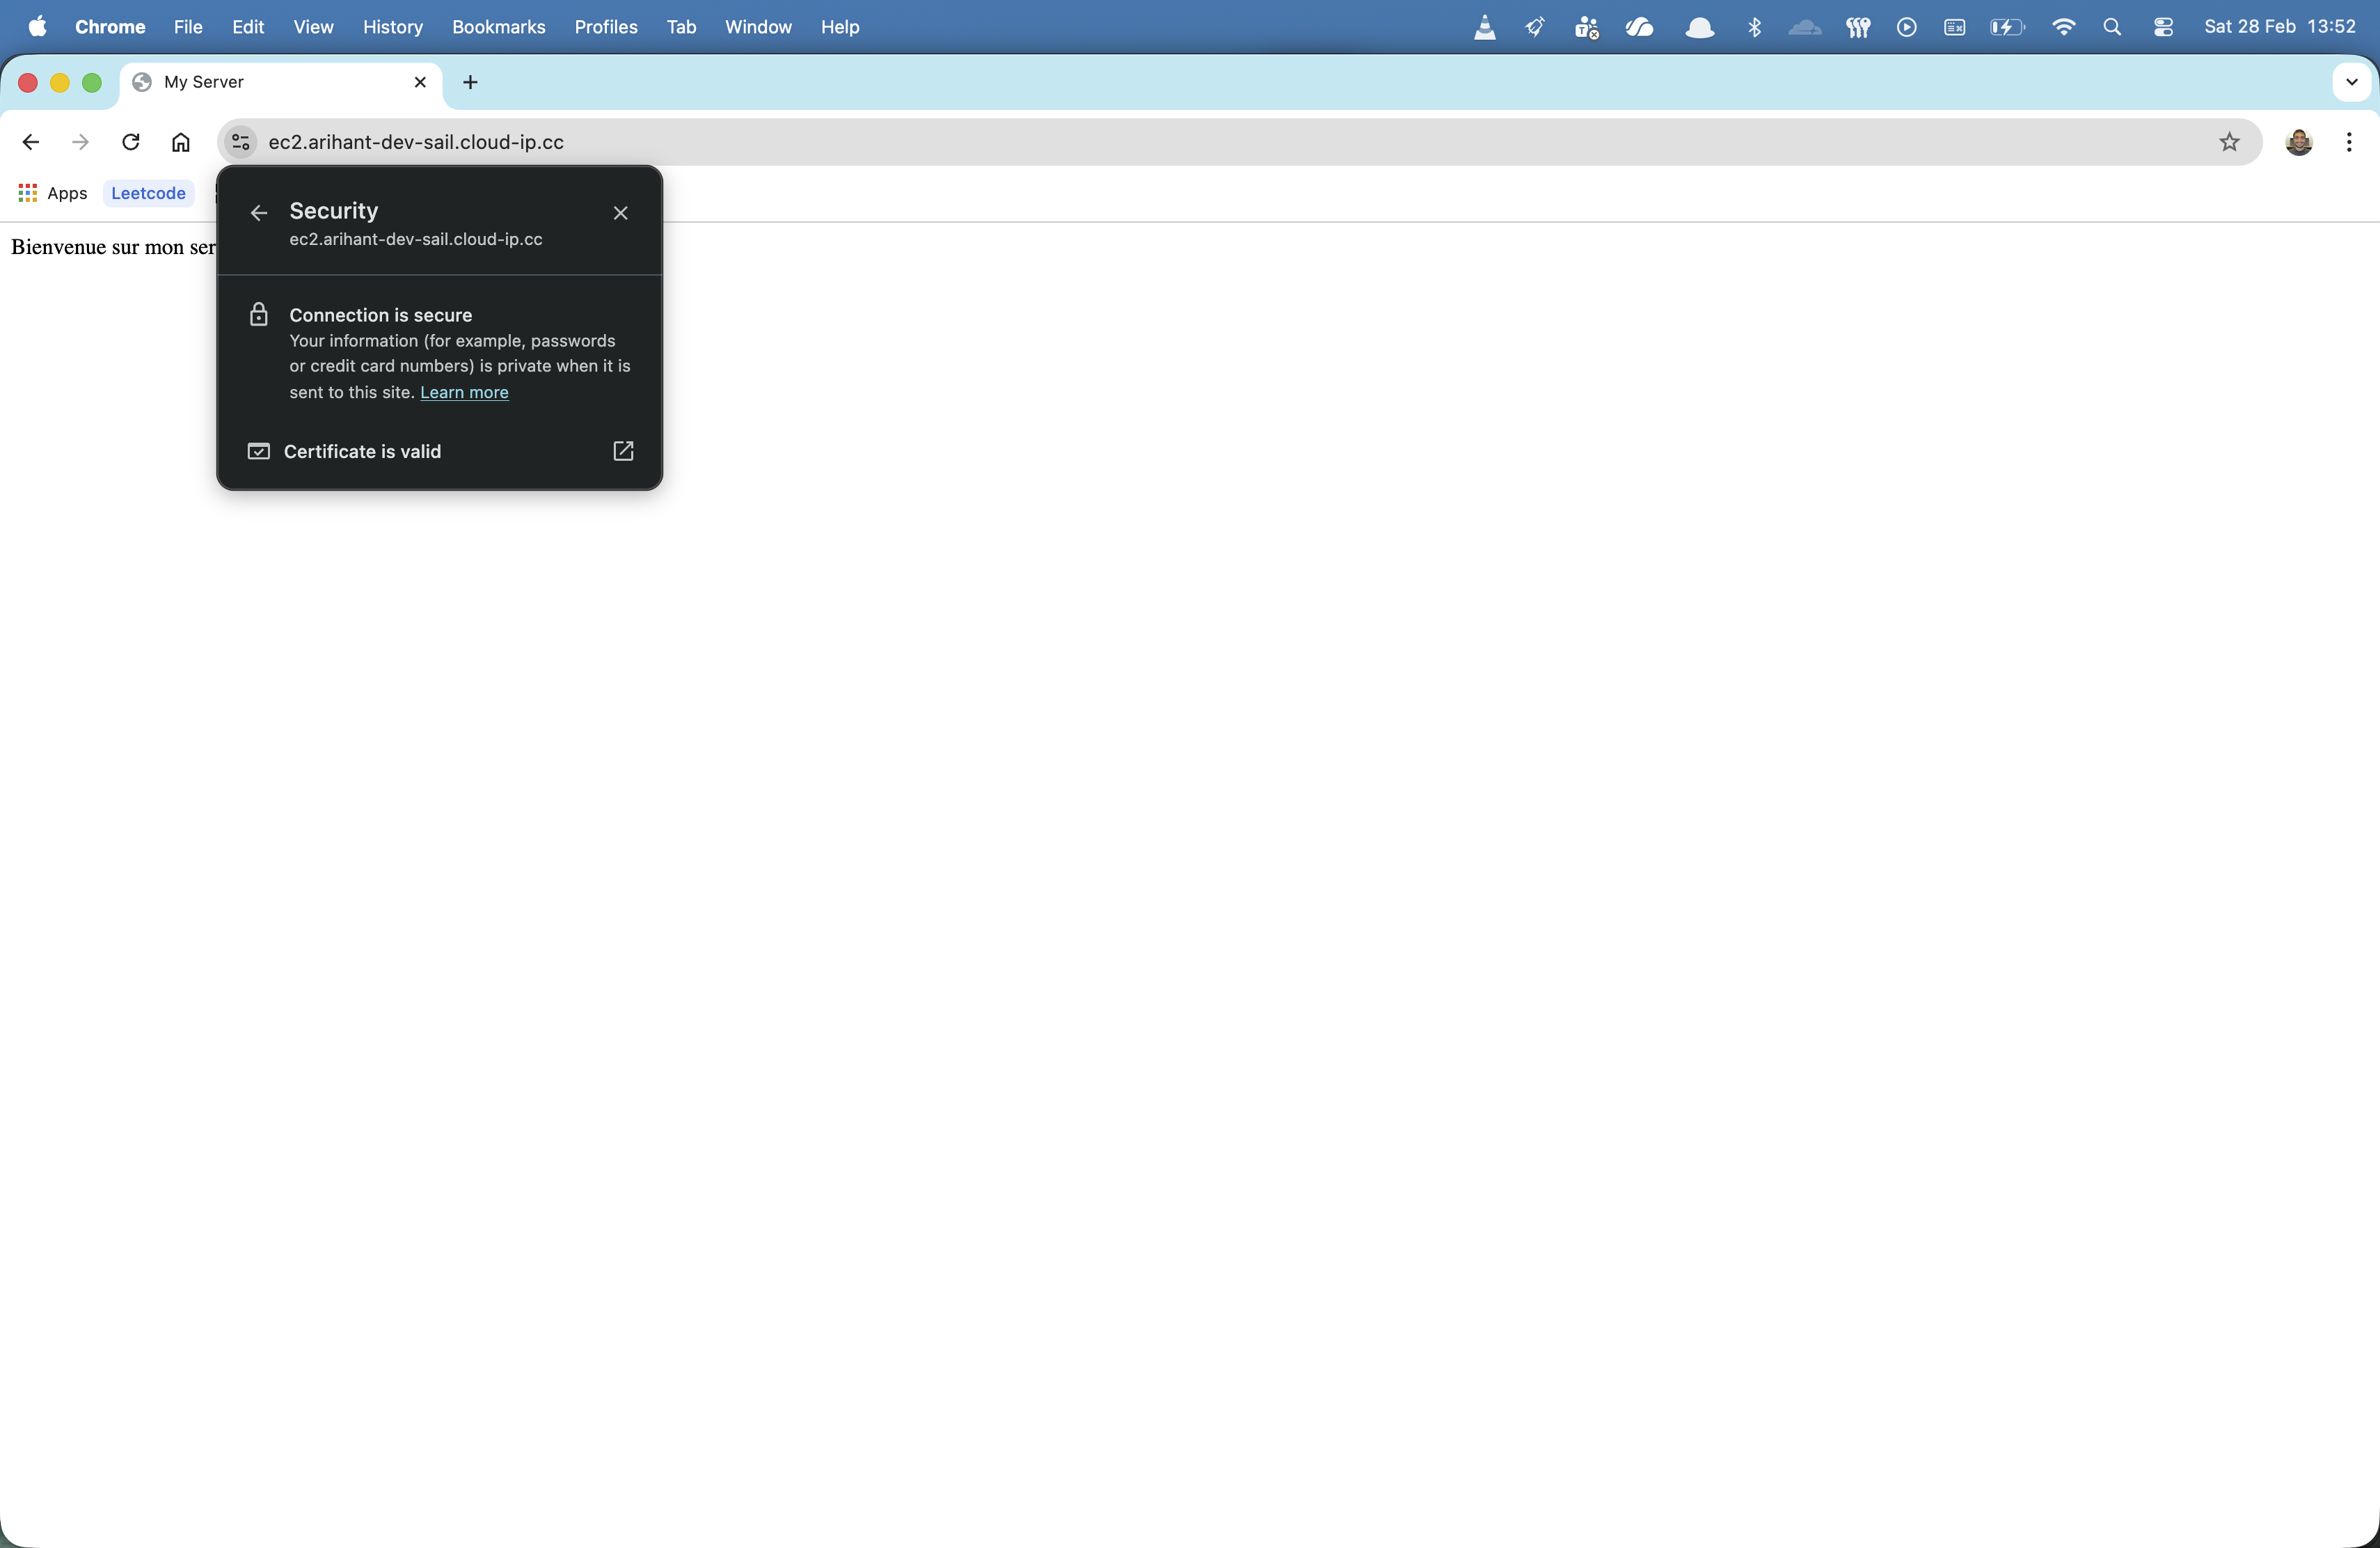
\includegraphics[width=0.65\textwidth]{figures/lets_encrypt_certificate.png}
    \caption{Valid Let's Encrypt certificate in the browser (Arihant Jain)}
\end{figure}

\subsection{Enable the Apache Rewrite Engine and Create the HTTP to HTTPS Redirect Rule. Test with a Web Browser}
To ensure all traffic is served over HTTPS, we enable the Apache rewrite module and configure an automatic redirect from HTTP to HTTPS:

\begin{lstlisting}[language=bash]
sudo a2enmod rewrite
sudo systemctl restart apache2
\end{lstlisting}

We then edit the Apache virtual host configuration for port 80:

\begin{lstlisting}[language=bash]
sudo nano /etc/apache2/sites-available/000-default.conf
\end{lstlisting}

Adding the following rewrite rules inside the \texttt{<VirtualHost *:80>} block:

\begin{lstlisting}[language=Bash]
<VirtualHost *:80>
    ServerName arihant-dev-sail.cloud-ip.cc
    RewriteEngine On
    RewriteCond %{HTTPS} off
    RewriteRule ^(.*)$ https://%{HTTP_HOST}%{REQUEST_URI} [R=301,L]
</VirtualHost>
\end{lstlisting}

After restarting Apache, any request to \texttt{http://arihant-dev-sail.cloud-ip.cc} is automatically redirected to \texttt{https://arihant-dev-sail.cloud-ip.cc}. Note that Certbot can also configure this redirect automatically when prompted during certificate installation.

\begin{figure}[H]
    \centering
    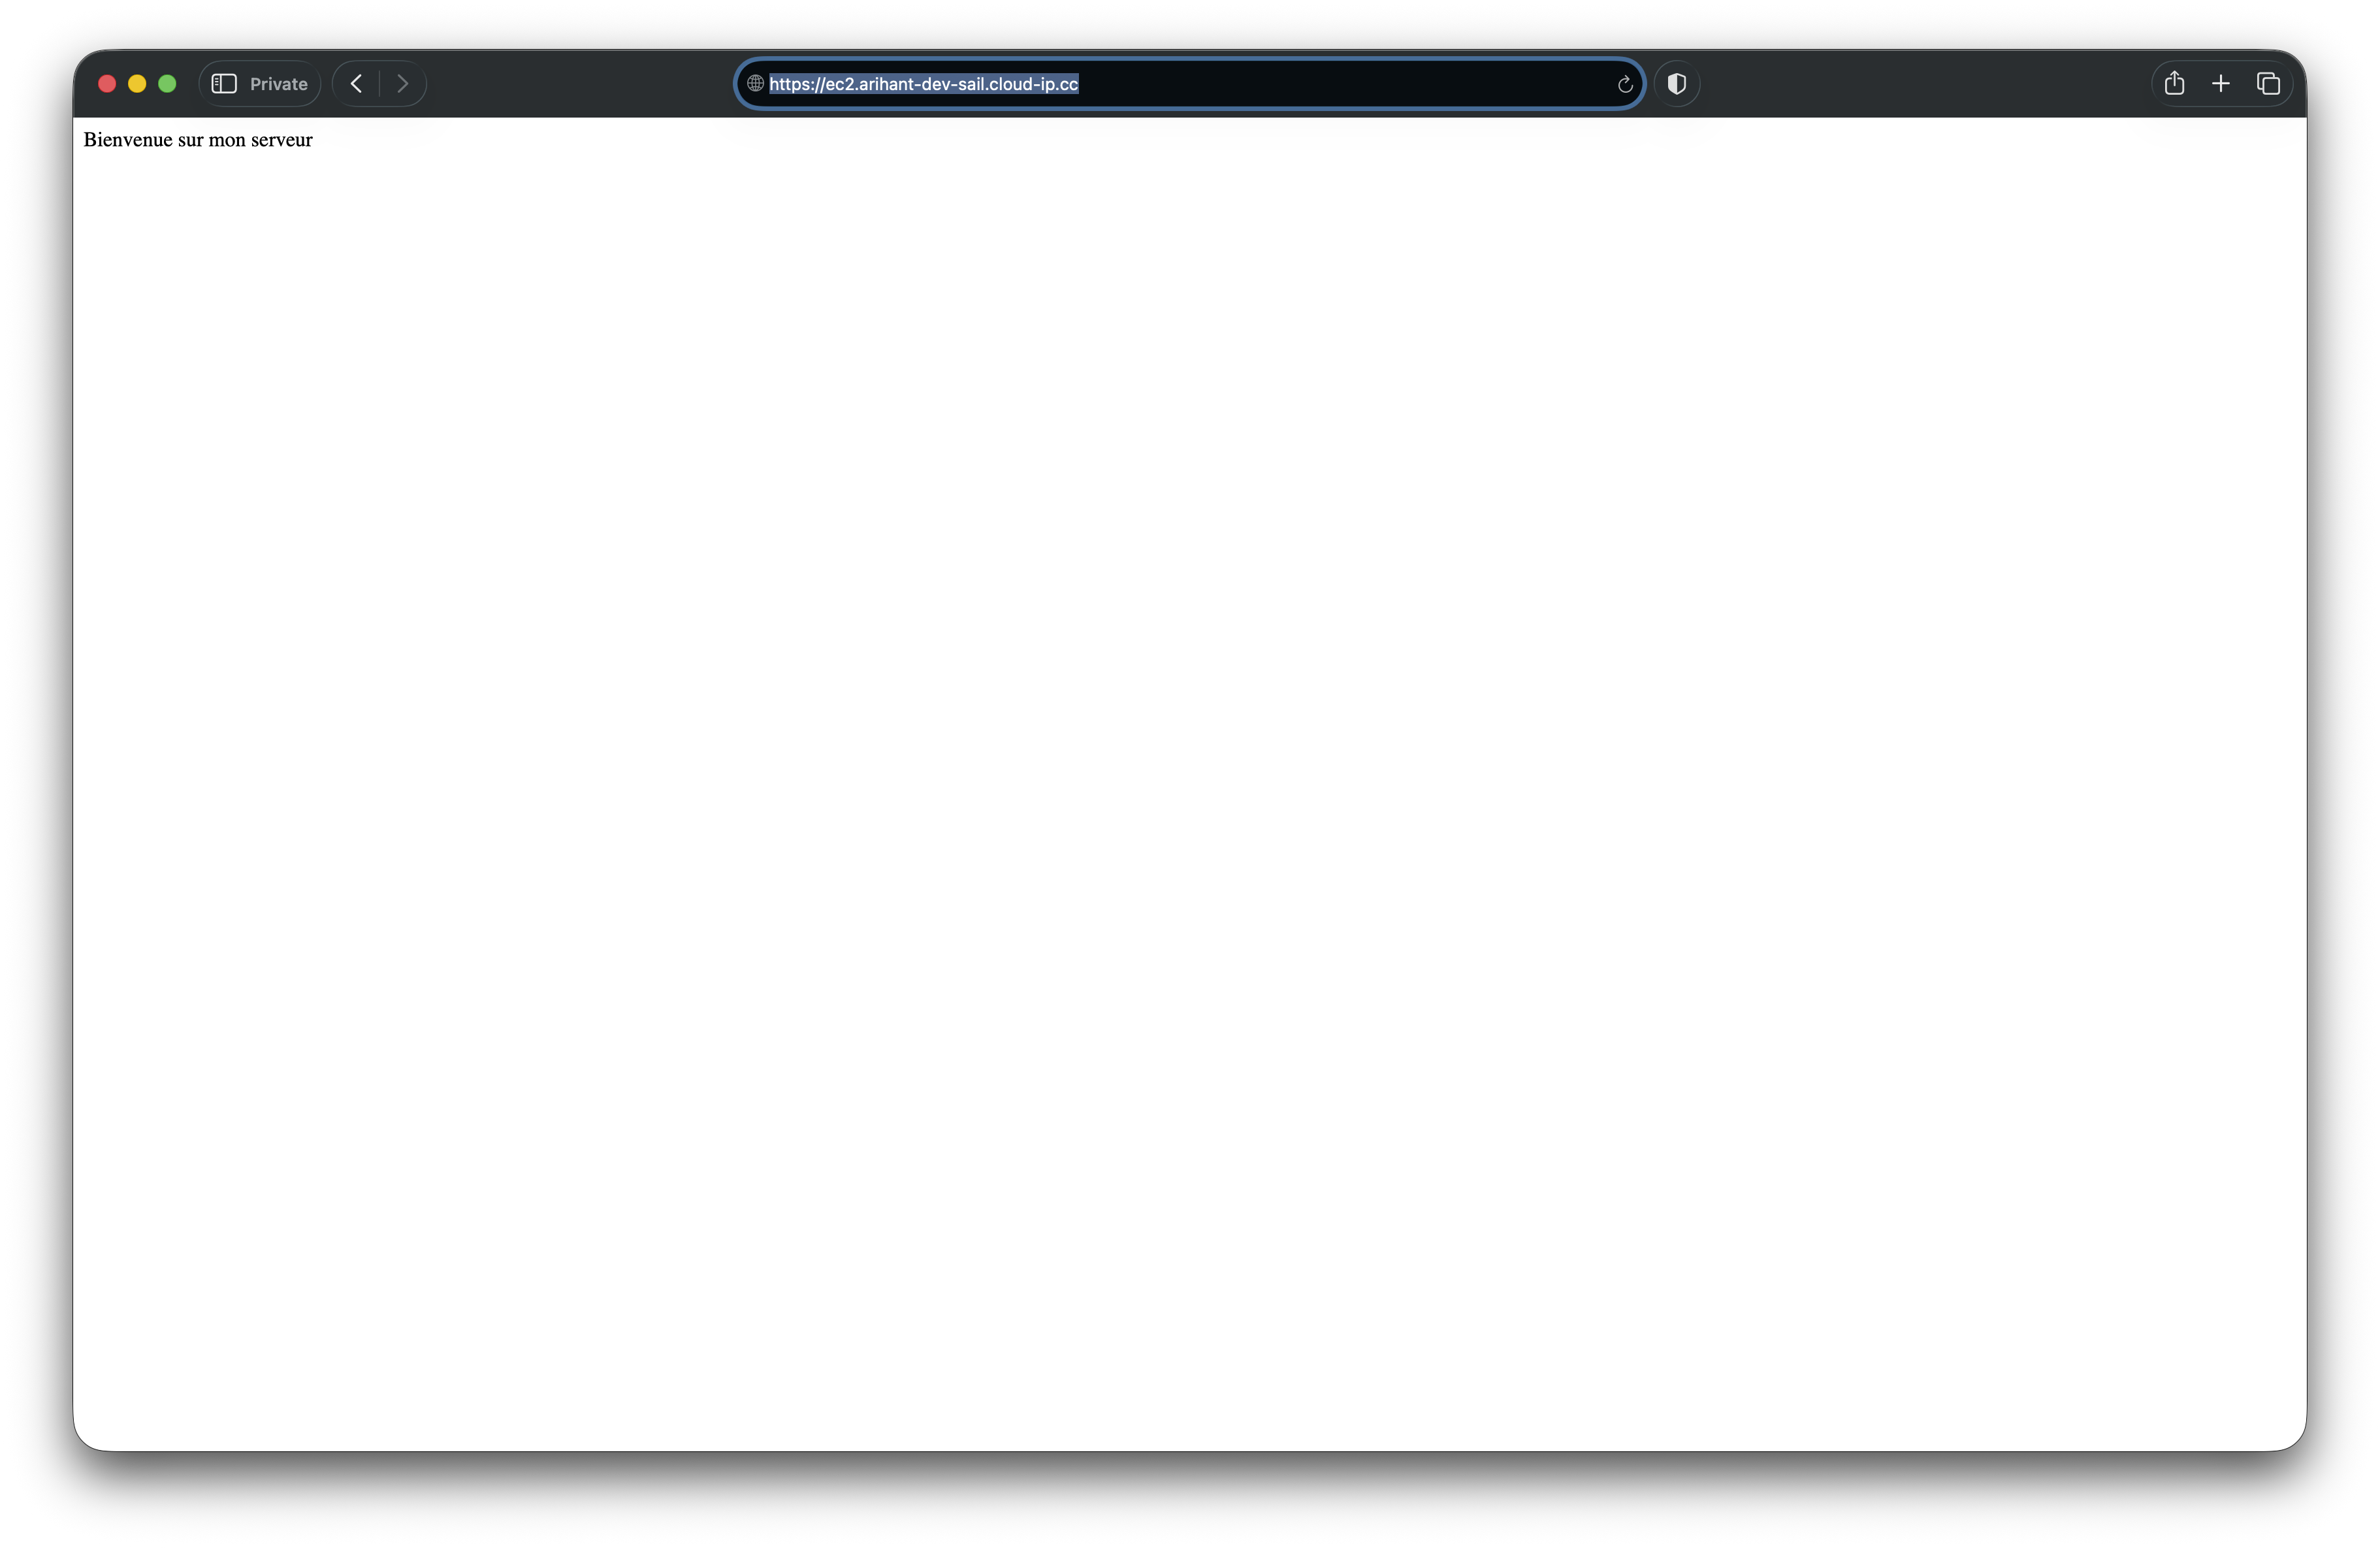
\includegraphics[width=0.65\textwidth]{figures/http_redirect.png}
    \caption{HTTP to HTTPS redirect working in the browser (Arihant Jain)}
\end{figure}

%% ============ SECTION 3: Creating a PHP Application ============ %%
\section{Creating a PHP Application}
\setcounter{subsection}{13}

\subsection{Install the PHP Module}
To serve dynamic content with Apache, we install PHP and the Apache PHP module:

\begin{lstlisting}[language=bash]
sudo apt install php libapache2-mod-php php-curl
sudo systemctl restart apache2
\end{lstlisting}

PHP is now installed and loaded as an Apache module, allowing the server to process \texttt{.php} files.

\subsection{Create a phpinfo.php Script and Identify the PHP Version}
To verify that PHP is correctly installed and configured with Apache, we create a test file:

\begin{lstlisting}[language=bash]
sudo nano /var/www/html/phpinfo.php
\end{lstlisting}

With the following content:

\begin{lstlisting}[language=PHP]
<?php
phpinfo();
?>
\end{lstlisting}

Navigating to \texttt{https://arihant-dev-sail.cloud-ip.cc/phpinfo.php} displays the full PHP configuration page. From this page, we can identify the PHP version currently installed on the server.

\begin{figure}[H]
    \centering
    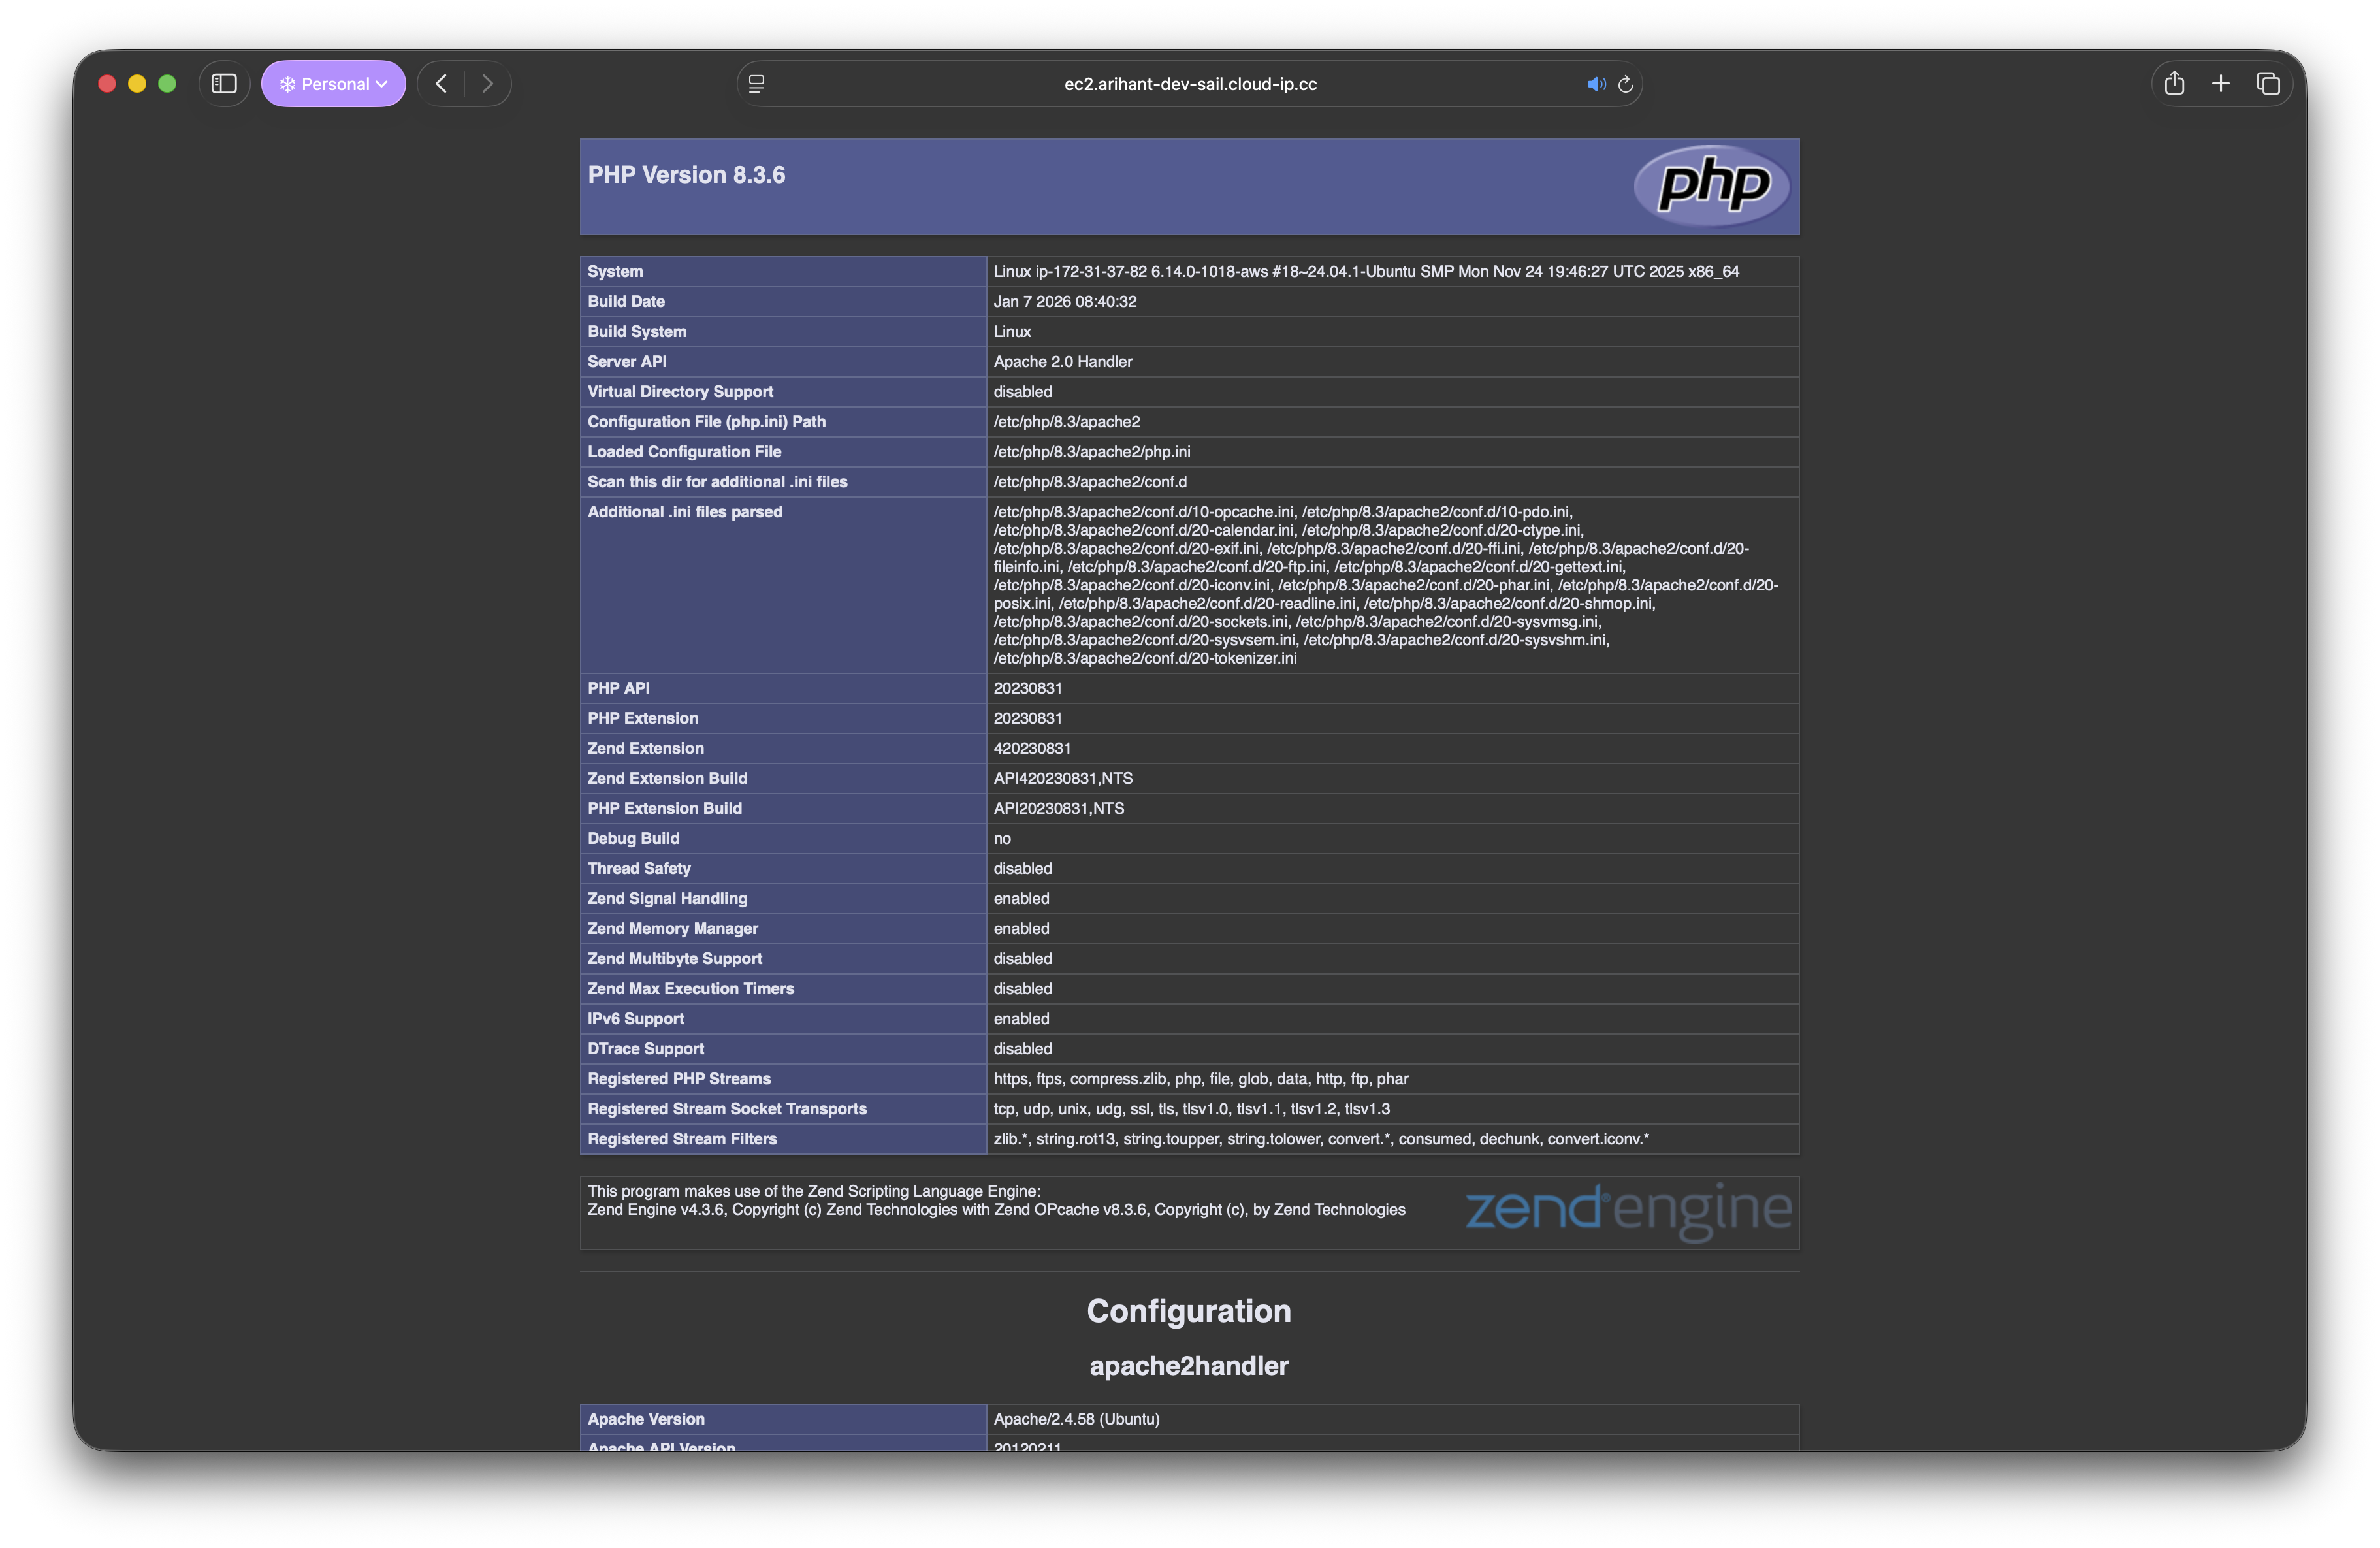
\includegraphics[width=0.65\textwidth]{figures/phpinfo.png}
    \caption{PHP info page showing the installed PHP version (Arihant Jain)}
\end{figure}

\subsection{Create a meteo.php Script That Displays Weather Information Using OpenWeather}
To build a weather application, we first set up an OpenWeatherMap API key:

\begin{enumerate}
    \item Create an account on \url{https://openweathermap.org}
    \item Navigate to the API keys section and generate a new key
    \item The API endpoint used is:
    \begin{center}
        \small\texttt{http://api.openweathermap.org/data/2.5/weather?q=\{city\}\&units=metric\&lang=fr\&appid=\{apiKey\}}
    \end{center}
\end{enumerate}

\begin{figure}[H]
    \centering
    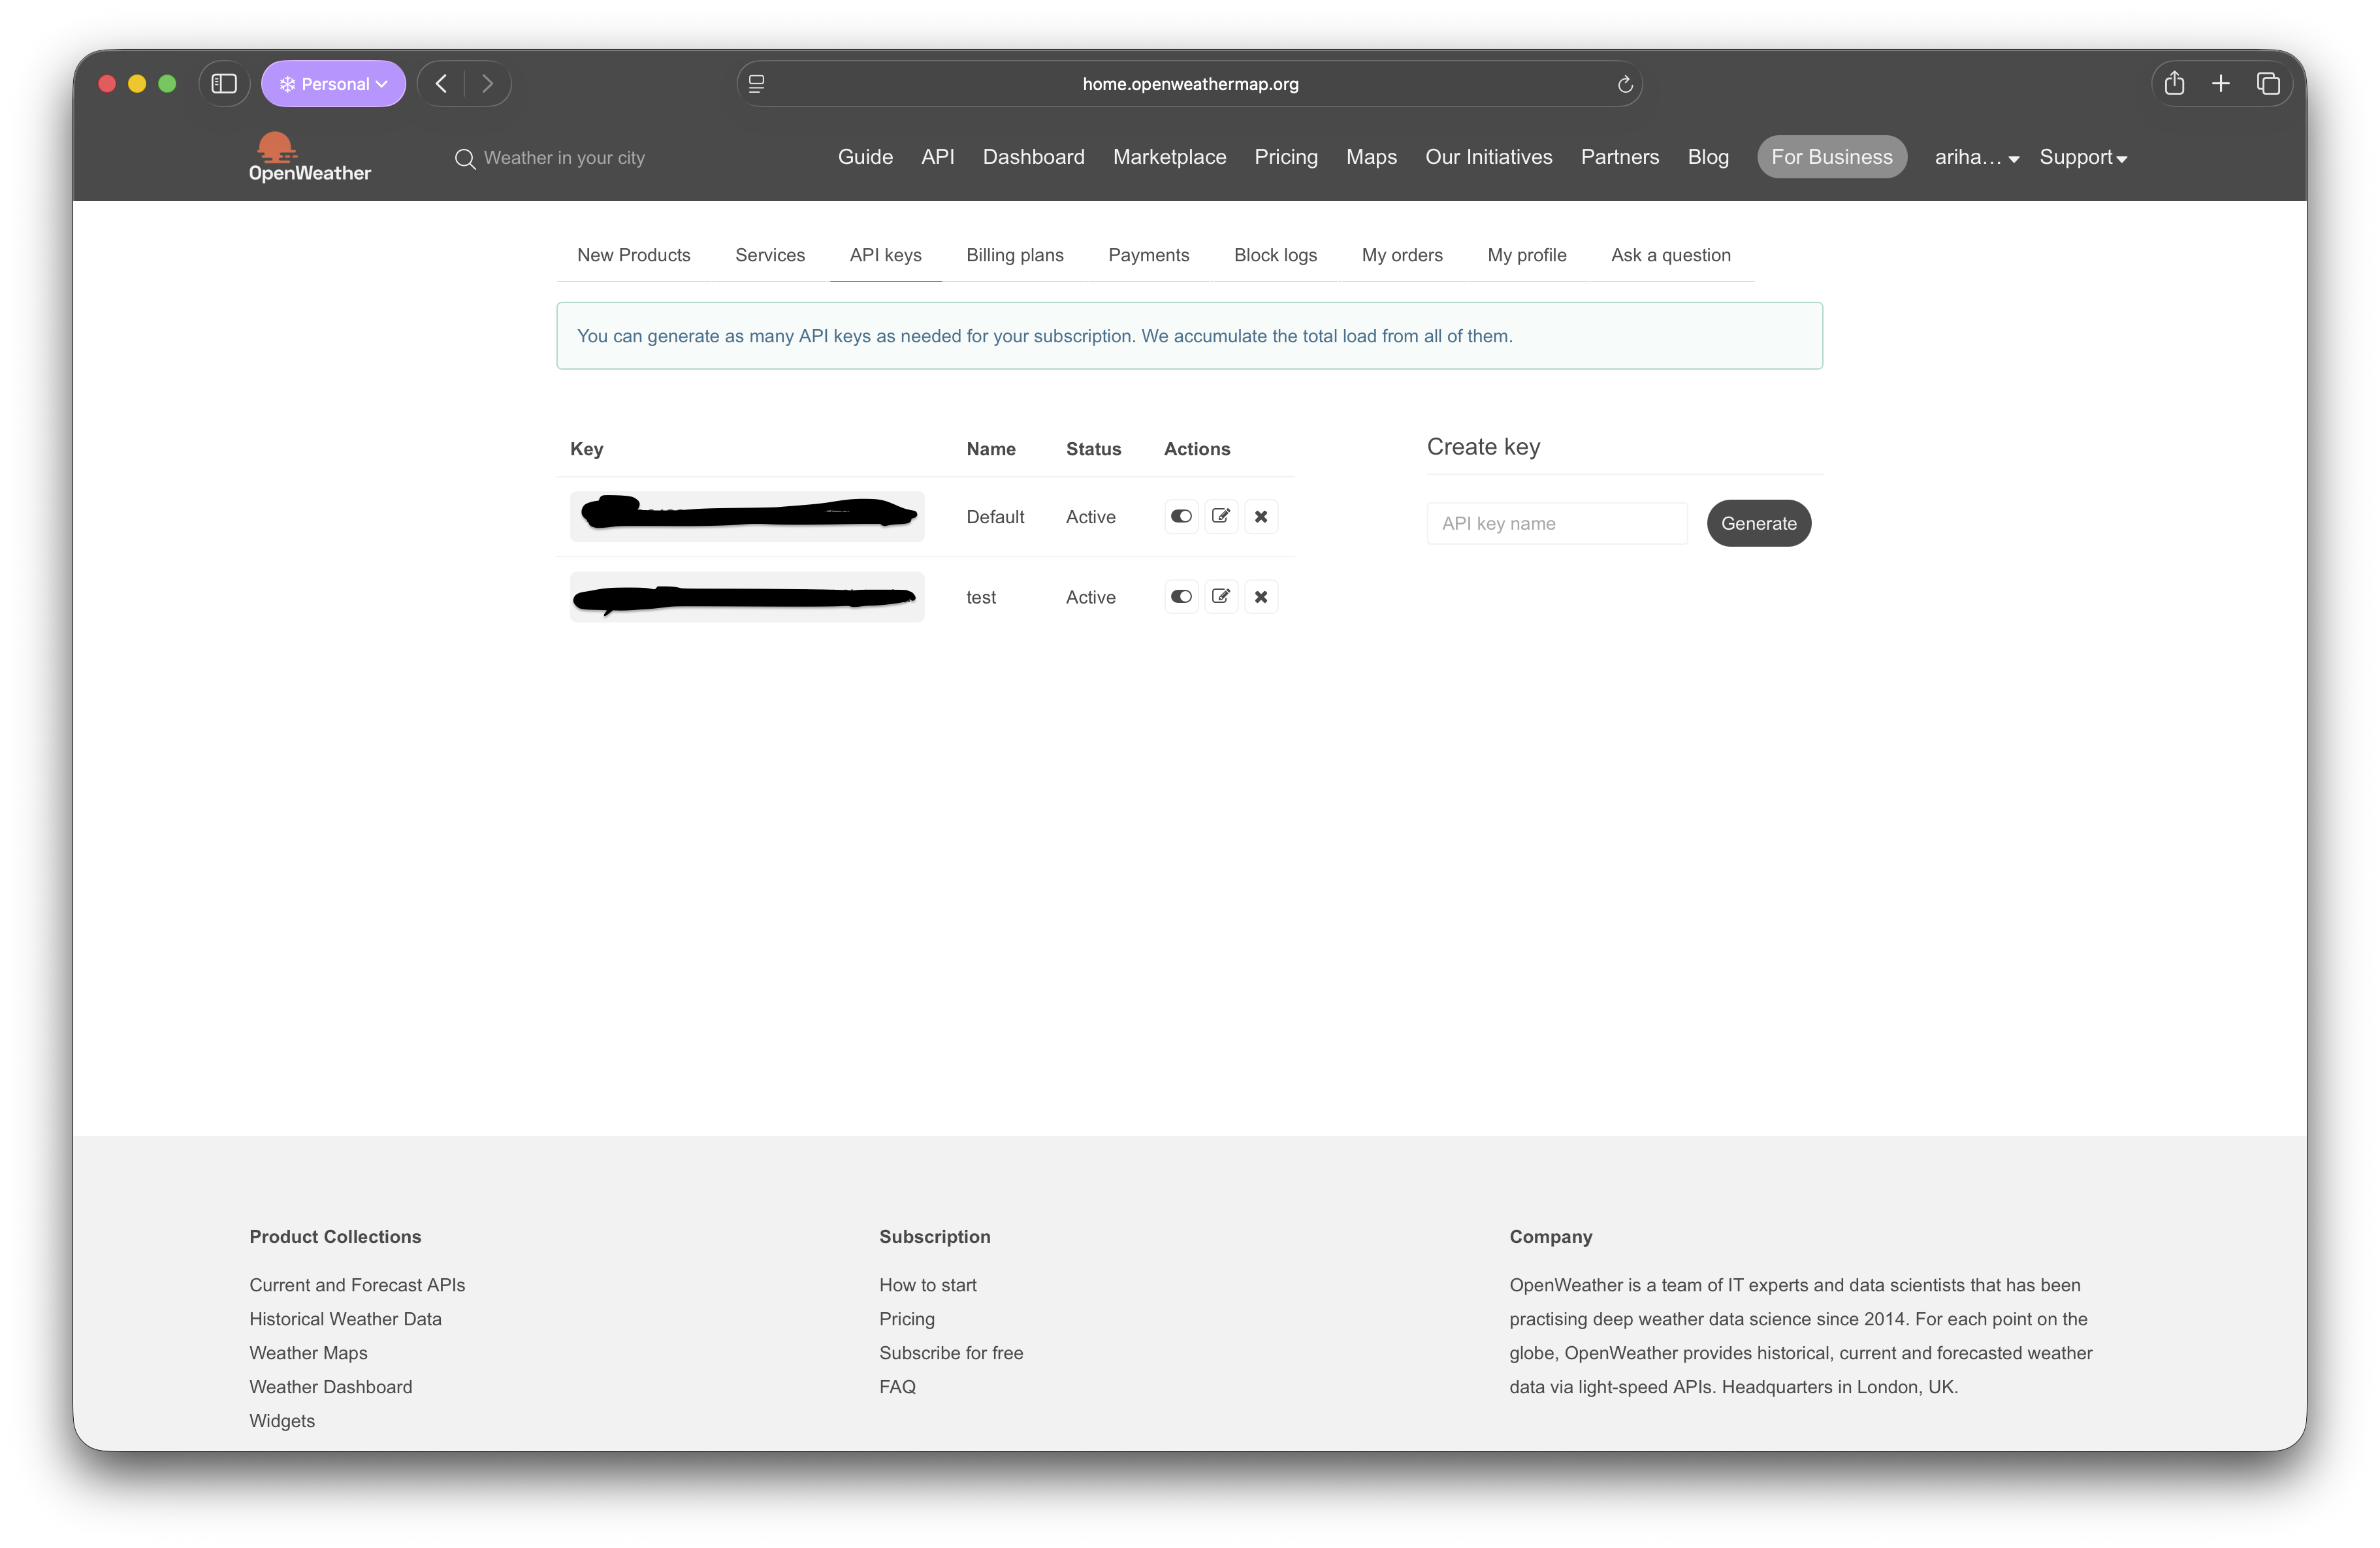
\includegraphics[width=0.65\textwidth]{figures/openweather_api.png}
    \caption{OpenWeatherMap API key dashboard (Arihant Jain)}
\end{figure}

We then create the weather application file:

\begin{lstlisting}[language=bash]
sudo nano /var/www/html/meteo.php
\end{lstlisting}

\vspace{7em}

The application fetches weather data for Paris using \texttt{file\_get\_contents()} to call the API and \texttt{json\_decode()} to parse the JSON response:

\begin{lstlisting}[language=PHP]
<?php
$apiKey = "YOUR_API_KEY";
$city = "Paris";

$url = "http://api.openweathermap.org/data/2.5/weather?q="
    . $city . "&units=metric&lang=fr&appid=" . $apiKey;

$response = file_get_contents($url);
$data = json_decode($response, true);

$temperature = $data['main']['temp'];
$description = $data['weather'][0]['description'];
$humidity = $data['main']['humidity'];
$windSpeed = $data['wind']['speed'];
?>

<!DOCTYPE html>
<html>
<head>
    <title>Meteo Paris</title>
</head>
<body>
    <h1>Meteo a <?php echo $city; ?></h1>
    <p>Temperature : <?php echo $temperature; ?> C</p>
    <p>Description : <?php echo $description; ?></p>
    <p>Humidite : <?php echo $humidity; ?>%</p>
    <p>Vent : <?php echo $windSpeed; ?> m/s</p>
</body>
</html>
\end{lstlisting}

The application is accessible at \texttt{https://arihant-dev-sail.cloud-ip.cc/meteo.php}. It calls the OpenWeatherMap API with the city set to Paris, retrieves the current temperature, weather description, humidity, and wind speed, and displays them on the page. The \texttt{units=metric} parameter ensures temperatures are in Celsius and \texttt{lang=fr} returns descriptions in French.

\begin{figure}[H]
\centering
\begin{minipage}{0.48\textwidth}
    \centering
    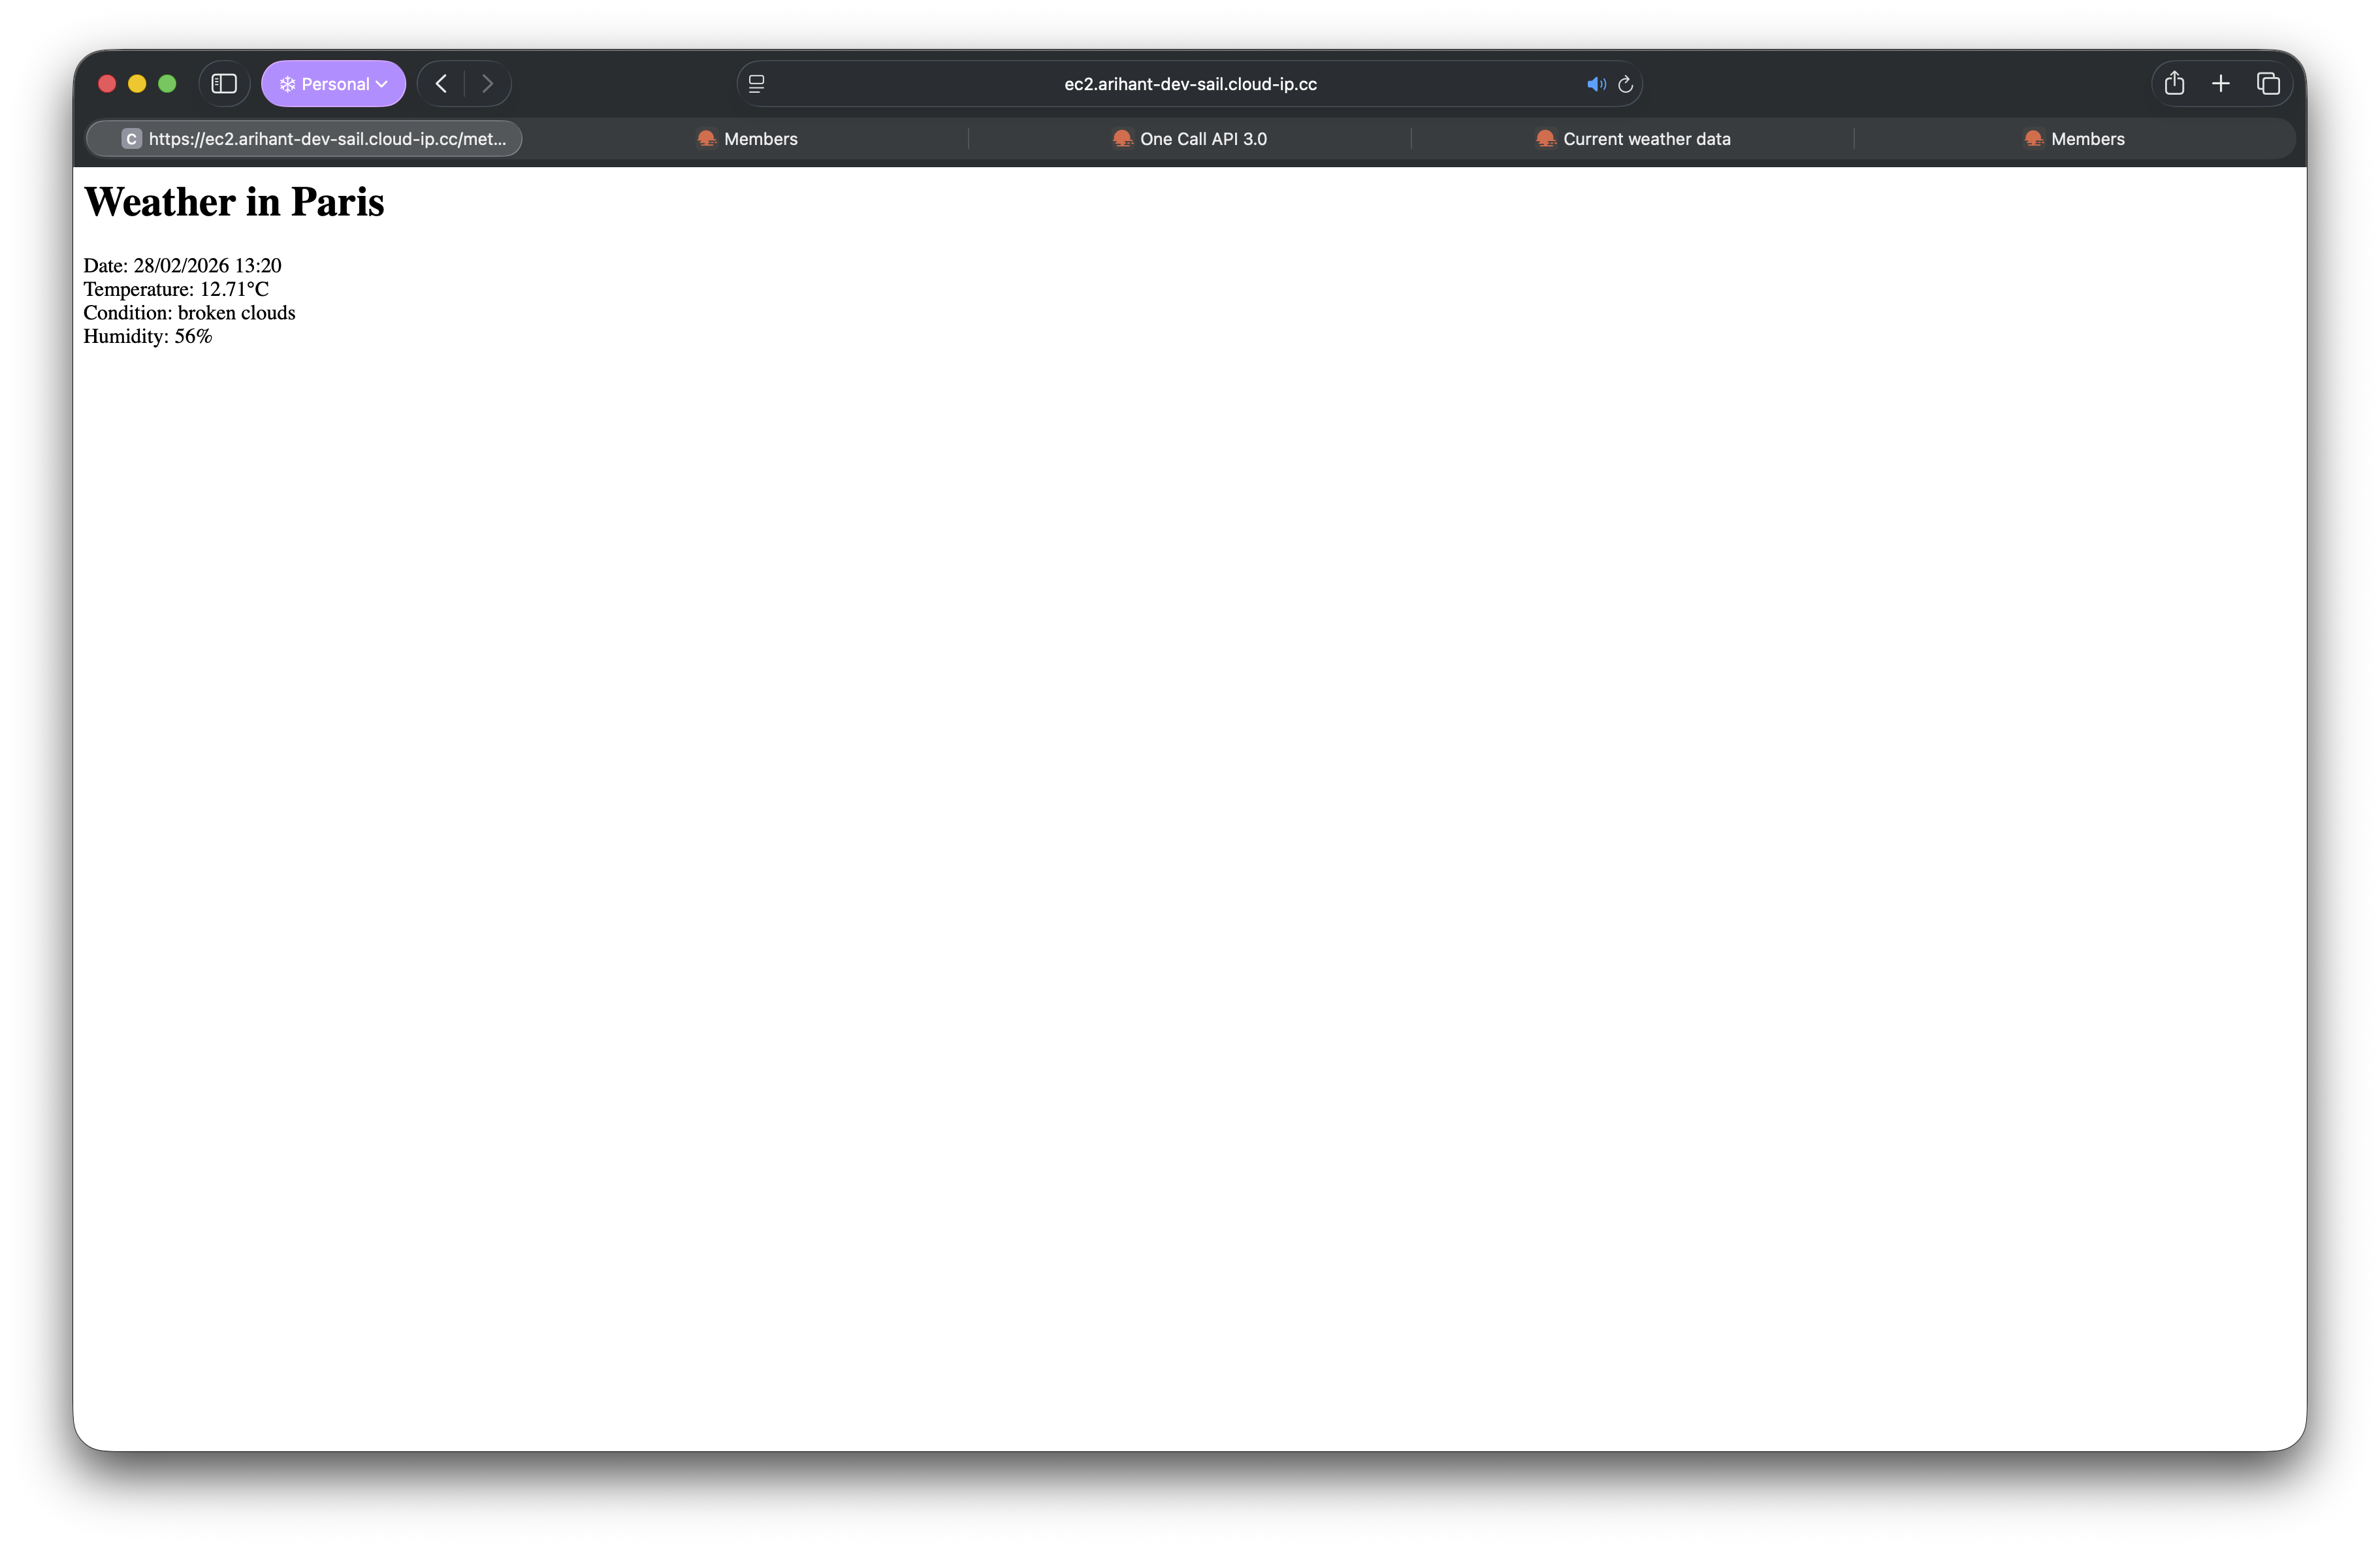
\includegraphics[width=\linewidth]{figures/weather_page_php.png}
    \captionof{figure}{Initial weather page (Arihant Jain)}
\end{minipage}\hfill
\begin{minipage}{0.48\textwidth}
    \centering
    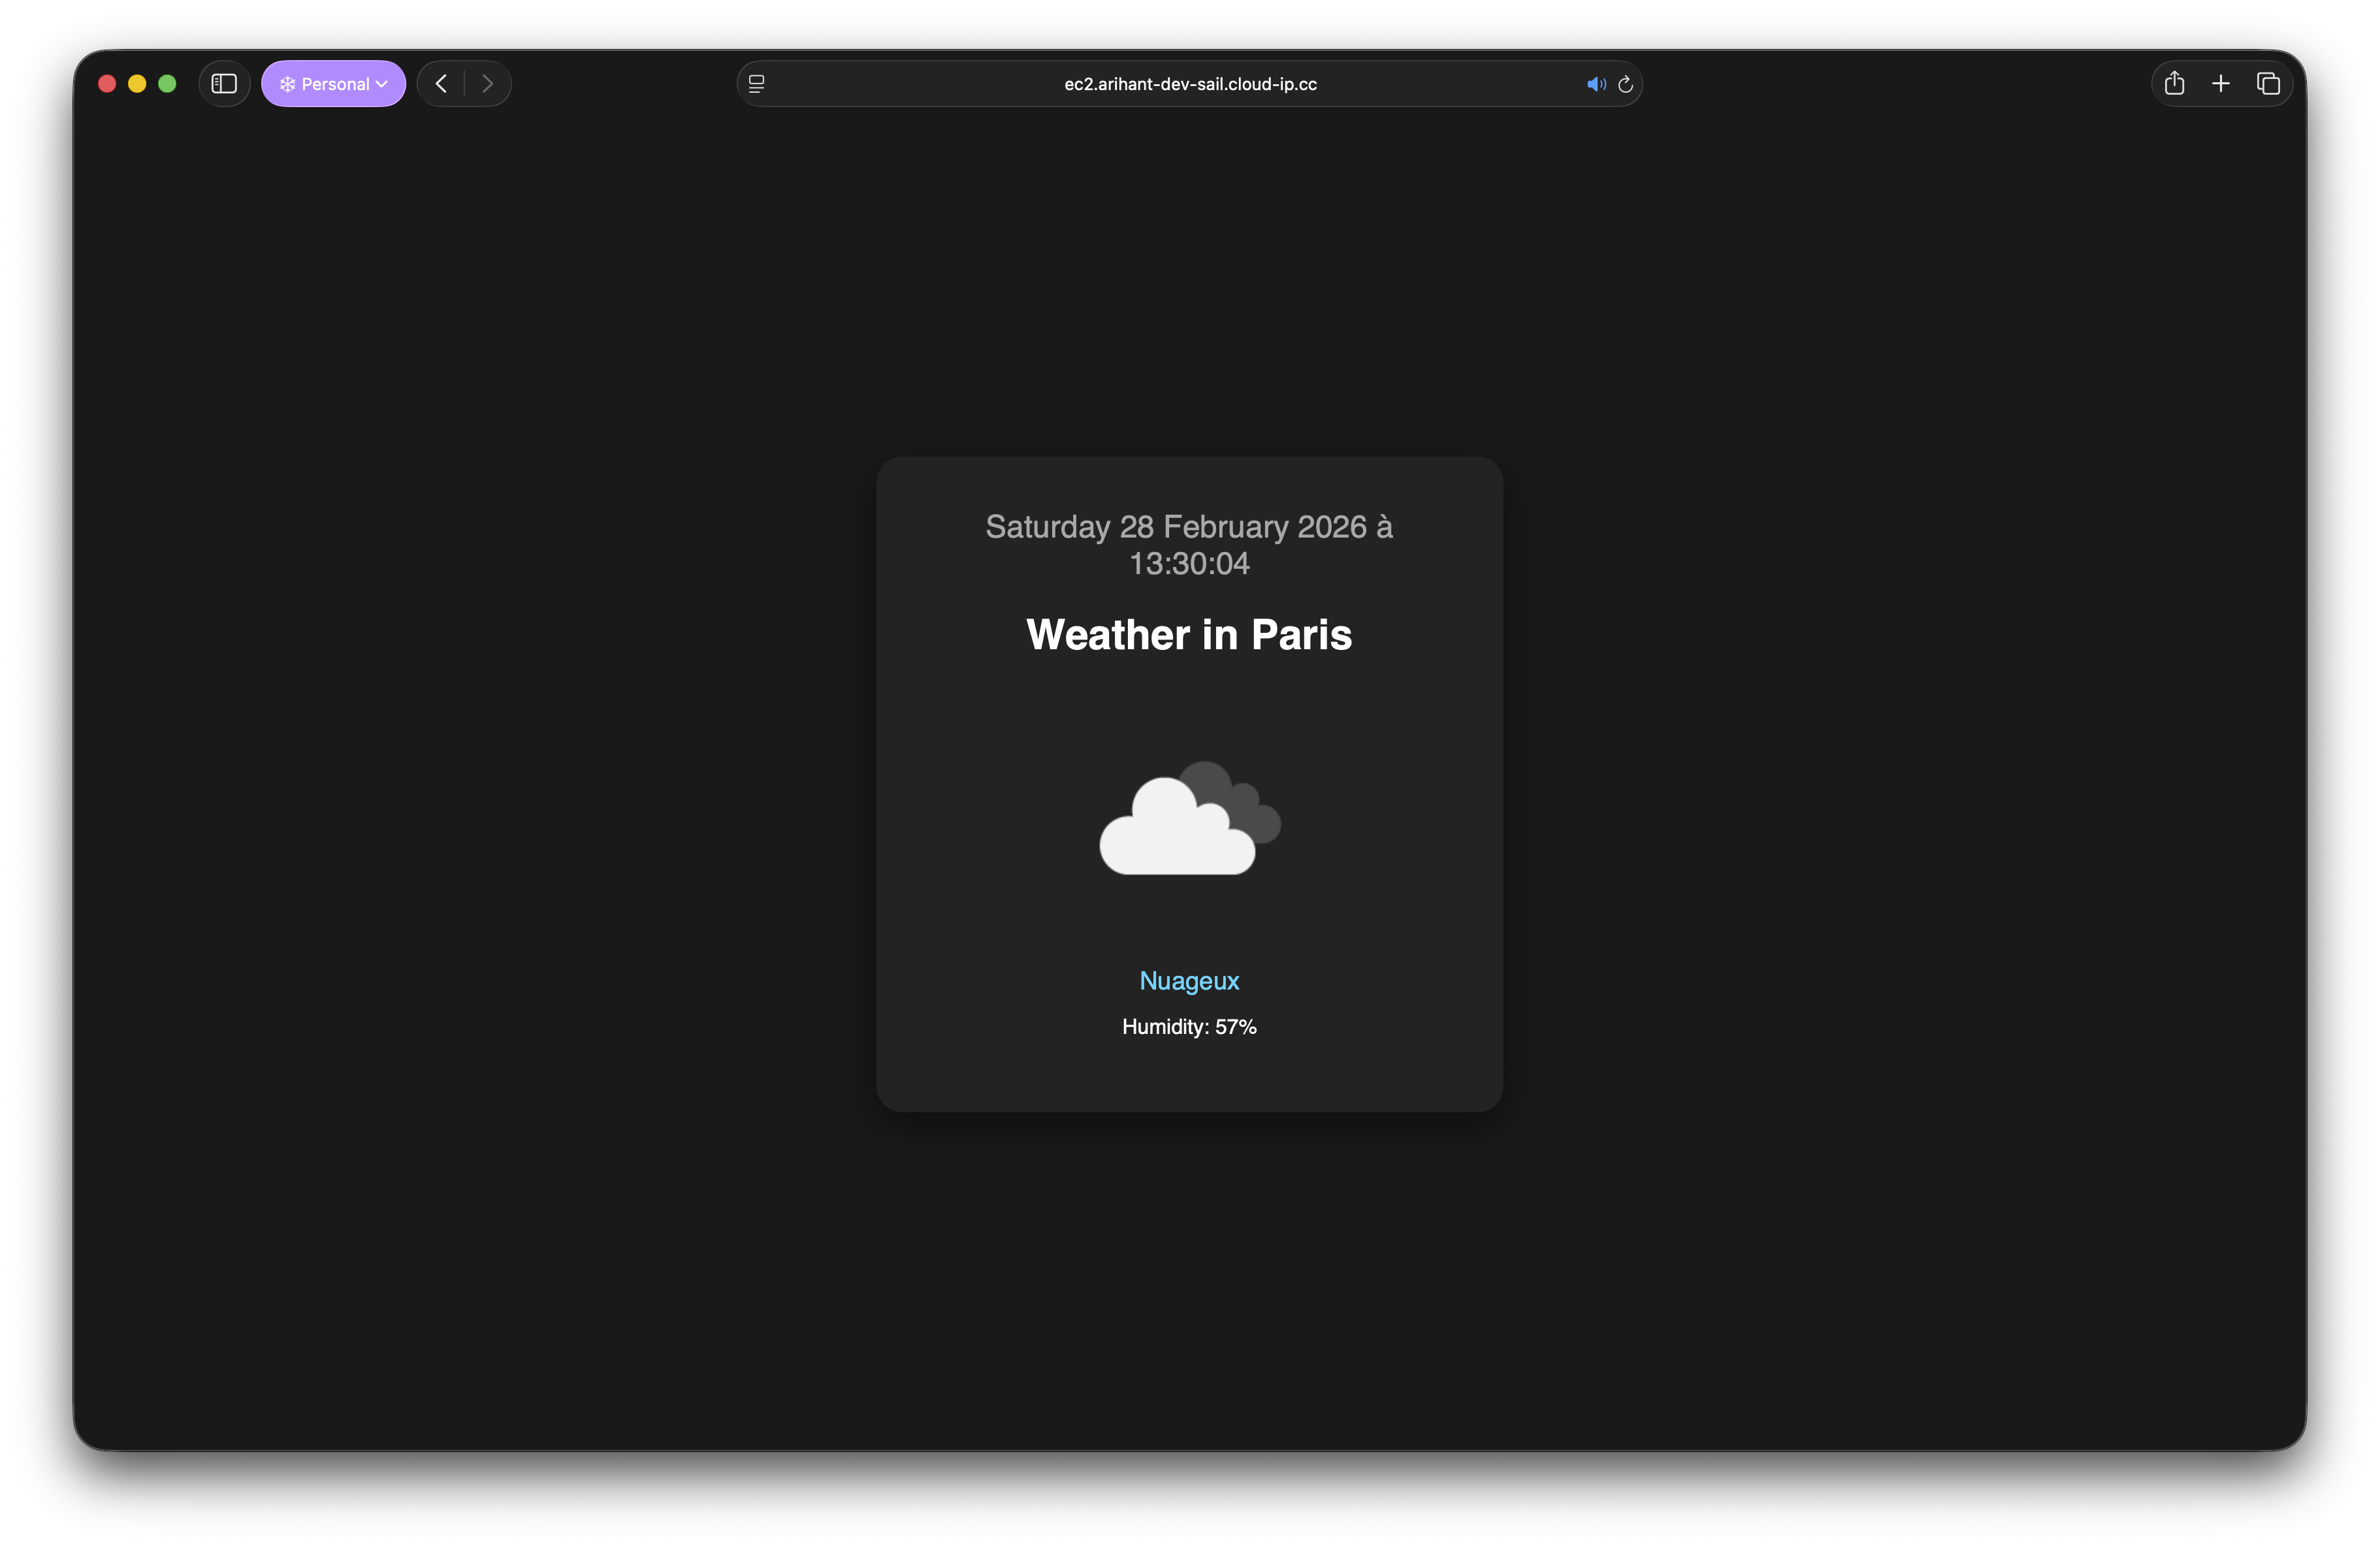
\includegraphics[width=\linewidth]{figures/updated_weather_page.png}
    \captionof{figure}{Updated weather page (Arihant Jain)}
\end{minipage}
\end{figure}

The left figure shows the initial version of the weather application displaying raw data from the API. The right figure shows the updated version with improved styling and layout for a better user experience.

\end{document}
